\documentclass[11pt,a4paper]{article}
\usepackage{fontspec}
\usepackage{xetexko}
\usepackage{amsmath,amssymb,amsthm}
\usepackage{unicode-math}
\usepackage[a4paper,margin=25mm]{geometry}
\usepackage{booktabs,longtable,tabularx,array}
\usepackage{enumitem}
\usepackage{xcolor}
\usepackage{graphicx}
\usepackage{tikz}
\usetikzlibrary{arrows.meta,positioning,fit,calc}
\usepackage{hyperref}
\usepackage[nameinlink,noabbrev]{cleveref}

\defaultfontfeatures{Ligatures=TeX}
\setmainfont{TeX Gyre Pagella}
\setsansfont{TeX Gyre Heros}
\setmonofont{Latin Modern Mono}[Scale=MatchLowercase]
\setmathfont{TeX Gyre Pagella Math}
\setmainhangulfont{Noto Serif CJK KR}
\setsanshangulfont{Noto Sans CJK KR}
\setmonohangulfont{Noto Sans Mono CJK KR}[Scale=MatchLowercase]

\definecolor{provedcolor}{HTML}{176B45}
\definecolor{partialcolor}{HTML}{9A6700}
\definecolor{specifiedcolor}{HTML}{315E9E}
\definecolor{blockedcolor}{HTML}{A43A3A}
\definecolor{deferredcolor}{HTML}{6B4FA1}
\definecolor{ink}{HTML}{1E293B}
\definecolor{softgray}{HTML}{F3F4F6}
\definecolor{analogycolor}{HTML}{0F766E}

\hypersetup{
  colorlinks=true,
  linkcolor=specifiedcolor,
  citecolor=provedcolor,
  urlcolor=specifiedcolor,
  pdftitle={HAETAE-2 구현 검증의 대수적 지도},
  pdfsubject={순수 대수학자와 대수기하학자를 위한 HAETAE top-down EasyCrypt 안내서},
  pdfauthor={HAETAE top-down EasyCrypt project}
}

\setlist[itemize]{leftmargin=2em,itemsep=0.28em,topsep=0.4em}
\setlist[enumerate]{leftmargin=2.3em,itemsep=0.28em,topsep=0.4em}
\renewcommand{\arraystretch}{1.18}
\renewcommand{\contentsname}{목차}
\renewcommand{\figurename}{그림}
\renewcommand{\tablename}{표}
\renewcommand{\refname}{참고문헌}
\setlength{\emergencystretch}{3em}
\setlength{\parindent}{1em}
\setlength{\parskip}{0.18em}

\newcolumntype{Y}{>{\raggedright\arraybackslash}X}
\newcolumntype{L}[1]{>{\raggedright\arraybackslash}p{#1}}

\theoremstyle{definition}
\newtheorem{definition}{정의}[section]
\newtheorem{translation}[definition]{번역 원리}
\newtheorem{verified}[definition]{검증된 명제(verified proposition)}
\newtheorem{openobligation}[definition]{미해결 의무}
\newtheorem{caution}[definition]{주의}
\newtheorem{question}[definition]{참여 질문}

\crefname{definition}{정의}{정의}
\crefname{translation}{번역 원리}{번역 원리}
\crefname{verified}{검증된 명제(verified proposition)}{검증된 명제(verified propositions)}
\crefname{openobligation}{미해결 의무}{미해결 의무}
\crefname{caution}{주의}{주의}
\crefname{question}{참여 질문}{참여 질문}

\newcommand{\identifier}[1]{\nolinkurl{#1}}
\newcommand{\sourcepath}[1]{\nolinkurl{#1}}
% EasyCrypt declarations are long and underscore-heavy.  Use the same
% proportional font as the surrounding text so long identifiers can wrap
% without consuming table width like typewriter text.
\newcommand{\theoremname}[1]{{\begingroup\urlstyle{same}\nolinkurl{#1}\endgroup}}
\newcommand{\claimid}[1]{\textsf{\textbf{\detokenize{#1}}}}
\newcommand{\statusproved}{\textcolor{provedcolor}{\textsf{\textbf{PROVED}}}}
\newcommand{\statuspartial}{\textcolor{partialcolor}{\textsf{\textbf{PARTIAL}}}}
\newcommand{\statusspecified}{\textcolor{specifiedcolor}{\textsf{\textbf{SPECIFIED}}}}
\newcommand{\statusblocked}{\textcolor{blockedcolor}{\textsf{\textbf{BLOCKED}}}}
\newcommand{\statusdeferred}{\textcolor{deferredcolor}{\textsf{\textbf{DEFERRED}}}}

\newcommand{\ZZ}{\mathbb{Z}}
\newcommand{\FF}{\mathbb{F}}
\newcommand{\BB}{\mathbb{B}}
\newcommand{\Rq}{R_q}
\newcommand{\Bytes}{\mathsf{Byte}}
\newcommand{\Mem}{\mathsf{Mem}}
\newcommand{\take}{\mathop{\mathrm{take}}}
\newcommand{\prefix}{\mathop{\mathrm{prefix}}}
\newcommand{\restrict}{\mathord{\upharpoonright}}
\newcommand{\Encode}{\mathop{\mathrm{Enc}}}
\newcommand{\Decode}{\mathop{\mathrm{Dec}}}
\newcommand{\obs}{\mathop{\mathrm{obs}}}
\newcommand{\Adv}{\mathop{\mathrm{Adv}}}

\newenvironment{takeaway}[1]
  {\begin{quote}\color{ink}\noindent\textbf{#1}\par\smallskip}
  {\end{quote}}

\newenvironment{analogy}
  {\begin{quote}\color{analogycolor}\noindent\textbf{비유(형식화된 정리(theorem) 아님).}\par\smallskip}
  {\end{quote}}

\tikzset{
  layernode/.style={
    draw=specifiedcolor,
    rounded corners=2pt,
    fill=specifiedcolor!6,
    align=center,
    minimum height=11mm,
    text width=35mm,
    inner sep=4pt
  },
  provennode/.style={
    draw=provedcolor,
    rounded corners=2pt,
    fill=provedcolor!7,
    align=center,
    minimum height=11mm,
    text width=38mm,
    inner sep=4pt
  },
  partialnode/.style={
    draw=partialcolor,
    dashed,
    rounded corners=2pt,
    fill=partialcolor!7,
    align=center,
    minimum height=11mm,
    text width=38mm,
    inner sep=4pt
  },
  blockednode/.style={
    draw=blockedcolor,
    dashed,
    rounded corners=2pt,
    fill=blockedcolor!5,
    align=center,
    minimum height=11mm,
    text width=38mm,
    inner sep=4pt
  },
  deferrednode/.style={
    draw=deferredcolor,
    densely dotted,
    rounded corners=2pt,
    fill=deferredcolor!6,
    align=center,
    minimum height=11mm,
    text width=38mm,
    inner sep=4pt
  },
  flowarrow/.style={-{Latex[length=2.2mm]},thick,draw=ink},
  openarrow/.style={-{Latex[length=2.2mm]},thick,dashed,draw=partialcolor}
}

% Snapshot metadata.  The 82-target paper surface remains frozen; the current
% branch also carries explicitly separated post-freeze EasyCrypt evidence.
\newcommand{\SnapshotDate}{2026년 8월 13일}
\newcommand{\SnapshotWeek}{PAPER--FREEZE 이후 faithful augmented KeyGen 계수곱 합성}
\newcommand{\AuthoredTargetCount}{82}
\newcommand{\WeekTenTargetCount}{6}
\newcommand{\WeekElevenTargetCount}{7}
\newcommand{\WeekTwelveTargetCount}{8}
\newcommand{\WeekThirteenTargetCount}{2}
\newcommand{\WeekFourteenTargetCount}{5}
\newcommand{\WeekFifteenTargetCount}{2}
\newcommand{\WeekSixteenTargetCount}{8}
\newcommand{\FrozenPaperGate}{\identifier{STOP-VERIFY-MATRIX-CRT}}
\newcommand{\CurrentGate}{\identifier{STOP-KG-AVEC-QJ}}
\newcommand{\FaithfulAugmentedVerdict}{\identifier{GO-KG-FAITHFUL-AUGMENTED}}
\newcommand{\CurrentPriority}{\claimid{OBL-KG-SECURITY-EXPANDVECA-SEMANTICS}: synthetic security ExpandVecA를 actual SHAKE128/rejection semantics로 교체·정제하는 정리(theorem)}
\newcommand{\ProjectMode}{HAETAE-2}


\title{\textbf{HAETAE-2 구현 검증의 대수적 지도}\\[0.4em]
  \Large 순수 대수학자와 대수기하학자를 위한 동반 안내서}
\author{HAETAE top-down EasyCrypt 작업 문서}
\date{상태 기준: \SnapshotDate\ (\SnapshotWeek)}

\begin{document}
\maketitle

\begin{abstract}
HAETAE-2는
\(R_q=\ZZ_q[X]/(X^{256}+1)\) 위의 모듈 격자 서명(module-lattice
signature)이다. 그러나 이 저장소에서 실제로 증명하는 대상은 환(ring) 자체에
머물지 않는다. 논문의 원소(element)와 모듈 사상(module map)을 정준
바이트열(canonical byte string)로 표현하고, 그 바이트열을 유한
메모리(finite memory)에 배치한 뒤, 실제 생성된
Jasmin 절차가 그 표현을 보존하거나 역산한다는 사실까지 내려간다. 이 문서는
그 과정을 ``대수적 대상(algebraic object)--표현 사상(representation
map)--상태기계(state machine) refinement''의 세 층으로
재구성한다.

최신 감사 기준선인 스냅샷 시점에는 \AuthoredTargetCount 개 authored
EasyCrypt 타깃이 manifest에 들어가 aggregate \identifier{-no-eco} fresh compile을
통과했다. Week~10의 rANS encoder 타깃 \WeekTenTargetCount 개에 이어
Week~11의 encoder closure 타깃 \WeekElevenTargetCount 개, Week~12의 decoder
semantic-refinement 타깃 \WeekTwelveTargetCount 개, Week~13의 actual core
composition 타깃 \WeekThirteenTargetCount 개가 추가되었다.
닫힌 핵심은 비밀키의
992바이트 검증키 접두부,
raw/internal Sign--Verify의 32바이트 \(\mu\) 일치, challenge suffix 흡수,
서명 prefix round trip, HBZ 계수(coefficient)--기호(symbol) leaf
역함수(inverse function), 실제 13-symbol rANS 표의
certificate, 순수 rANS 단계와 byte-stack 정리(theorem), 실제 suffix copy,
encoder--decoder harness의 제어, 그리고 actual encoder 성공 출력 전체와 순수
\(\operatorname{TraceBytes}(\operatorname{SymbolList}(symbols_0))\) 사이의 정확한
등식(equality), exact trace에서 1024개 기호(symbol)를 복원하는 actual decoder
정제(refinement), 그리고 두 정리(theorem)와 actual suffix copy를
\identifier{Mode2RansActualHarness.run}에서 합성한 core 역함수(inverse function)다.
마지막 정리(theorem)는 encoder 성공을 전제로 요구하지 않고, 실패 시 decoder를
실행하지 않는 가지(branch)와 성공 시 1024개 기호(symbol)를 복원하는 가지를 함께
보이는 성공 조건부 부분정확성(success-conditioned partial correctness)이다.
반면 실제 encoder 성공 증인(success witness), encoder/decoder 종료성(termination),
production full-HBZ wrapper, 전체 suffix codec, 완료된 API trace의 저장
\(\mu\)를 연결하는 product/replay 운송, 전체 기능정확성과 구현 수준 보안은
열려 있다. 따라서 이 문서는 완성 증명을 선언하지 않고, 정확히 어디까지
commuting diagram이 닫혔는지를 표시한다.
\end{abstract}

\begin{takeaway}{한 문장 요약}
현재 성과는 환(ring) 위의 전체 서명 스킴(signature scheme)을 이미 검증했다는
뜻이 아니라, 그 스킴의 몇몇 결정론적 표현 사각형(representation square)이
실제 생성 코드까지 가환(commute)함을 증명했고, 다음 핵심
gate가 \CurrentPriority\ 임을 뜻한다. \CurrentGate 는 encoder와 decoder의
개별 간선(edge)에 이어 actual suffix copy를 통한 core 가환사각형(commutative
square)까지 닫혔다는 판정이다. production full-HBZ wrapper나 전체 codec이
완료됐다는 판정은 아니다.
\end{takeaway}

\tableofcontents
\clearpage

\section{독자 계약과 전체 지도}
\label{sec:reading-contract}

\subsection{이 문서가 가정하는 것과 설명하는 것}

이 문서는 독자가 환(ring), 몫환(quotient ring), 자유 모듈(free module),
동치관계(equivalence relation)와 몫집합(quotient set),
가환도식(commutative diagram), 귀납법(induction)에 익숙하다고 가정한다.
수학 용어는 이처럼 문서의 첫 등장과 표제·도표·용어 사전에서 한국어 뒤에 영어 원어를
병기한다. 같은 문맥에서 반복할 때에는 가독성을 위해 한국어만 쓸 수 있다. 반대로
다음 지식은 가정하지 않는다.

\begin{itemize}
  \item HAETAE 또는 모듈 격자 서명(module-lattice signature)의 설계;
  \item Jasmin의 문법과 메모리 모델;
  \item EasyCrypt의 Hoare logic, pRHL, 전술 언어;
  \item rANS entropy coding의 구현 관례.
\end{itemize}

목표는 모든 소스 코드를 줄마다 설명하는 것이 아니다. 각 증명 의무에 대해
``대상(object)은 무엇인가'', ``어떤 사상(map)이 가환(commute)해야 하는가'',
``정의역(domain)을 제한하는 전제(premise)는 무엇인가'', ``현재 어느
화살표(arrow)까지 실제 절차에 대해 증명되었는가''를
답하는 것이 목표다. 프로젝트의 범위는 mode~2와 고정된 명세·구현 스냅샷에
한정된다 \cite{project-scope}.

\begin{translation}[세 층 번역]
저장소의 정리(theorem)는 다음 세 층을 오가는 명제(proposition)로 읽는다.
\begin{enumerate}
  \item \textbf{대수 층(algebraic layer)}: \(R_q\)-모듈(module) 원소,
        분해(decomposition), challenge, 논문 알고리즘;
  \item \textbf{표현 층(representation layer)}: 정준 바이트열(canonical byte
        string), 접두부 투영(prefix projection), 메모리 구간(memory region),
        고정폭 정수(fixed-width integer);
  \item \textbf{실행 층(execution layer)}: 실제 생성 절차, 분기, 루프,
        반환값과 trace 관측값(observation).
\end{enumerate}
한 층에서 성립하는 등식(equality)을 다른 층으로 올리거나 내리려면 반드시 명명된
representation/refinement 정리(theorem)가 필요하다. 같은 수학적 의도를 구현한다는
사실만으로 도식(diagram)이 자동으로 가환(commute)하지 않는다.
\end{translation}

\begin{figure}[ht]
\centering
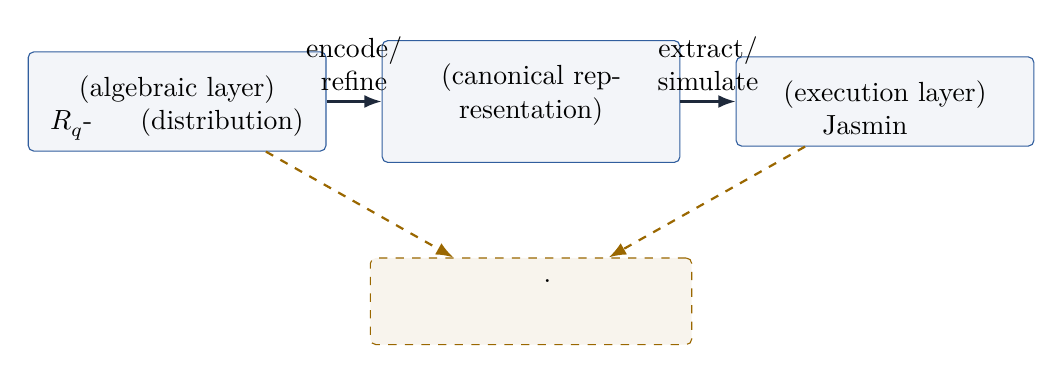
\begin{tikzpicture}[node distance=8mm and 7mm]
  \node[layernode] (alg) {논문 대수 층\\(algebraic layer)\\\(R_q\)-모듈과 분포(distribution)};
  \node[layernode, right=of alg] (repr) {정준 표현 층\\(canonical representation)\\바이트열과 접두부};
  \node[layernode, right=of repr] (proc) {실제 실행 층\\(execution layer)\\Jasmin 상태기계};
  \node[partialnode, below=12mm of repr] (security) {최상위 기능·보안\\합성 목표};
  \draw[flowarrow] (alg) -- node[above,align=center]{encode/\\refine} (repr);
  \draw[flowarrow] (repr) -- node[above,align=center]{extract/\\simulate} (proc);
  \draw[openarrow] (proc) -- (security);
  \draw[openarrow] (alg) -- (security);
\end{tikzpicture}
\caption{전체 증명 구조. 수평 화살표의 일부만 닫혔고, 최상위 합성 화살표는
아직 부분적이다.}
\label{fig:three-layers}
\end{figure}

\subsection{상태어는 논리적 양화사(quantifier)를 포함한다}

운영상 source of truth는 \sourcepath{CLAIM_LEDGER.md}이며
\cite{claim-ledger}, 의존성은 \sourcepath{THEOREM_GRAPH.md}에 기록된다
\cite{theorem-graph}. 이 문서에서 상태어는 다음 의미로만 사용한다.

\begin{center}
\begin{tabularx}{\textwidth}{L{28mm} Y Y}
\toprule
표시 & 정확한 뜻 & 자동으로 따라오지 않는 것 \\
\midrule
\statusproved & 표시된 전제 아래 명명된 EasyCrypt 선언이 fresh-compile된다. &
부모 주장, 종료성(termination), losslessness,
분포 동일성(distributional equality) \\
\statuspartial & 자식 명제(proposition) 또는 제한된 방향은 증명되었지만 명명된 부모가 열려 있다. &
제한을 제거한 전역 명제(global statement) \\
\statusspecified & 목표를 나타내는 연산(operation)·술어(predicate)·인터페이스가
컴파일된다. &
그 목표의 증명 \\
\statusblocked & 구체적인 extraction, 의미론(semantics), 수치·확률 정리(theorem)가 없어
합성할 수 없다. &
난점이 해결 불가능하다는 주장 \\
\statusdeferred & 시간 제한 뒤 명시적인 논문 경계로 동결했다. &
거짓 또는 불필요하다는 주장 \\
\bottomrule
\end{tabularx}
\end{center}

특히 ``Hoare partial correctness가 증명되었다''는 문장은
\[
  \text{절차가 반환한다면 사후조건이 성립한다}
\]
는 뜻이다. 절차가 모든 입력에서 반환한다거나, 확률적 재시도가 거의 확실히
끝난다는 뜻이 아니다. 이 구분은 KeyGen과 Sign의 rejection loop 때문에
본질적이다.

\subsection{대수기하학은 어디까지 관련되는가}

\(R_q\)는 물론 아핀 스킴(affine scheme) \(\operatorname{Spec}R_q\)를
정의한다. 또한 메모리의 부분구간 제한(local restriction), 국소 등식(local
equality), frame 조건은 제한사상(restriction map)과 접합(gluing)을 떠올리게
한다. 그러나 현재 EasyCrypt 파일은 스킴(scheme), 다형체(variety),
스펙트럼(spectrum), 층(sheaf), 코호몰로지(cohomology)를 형식화하지 않는다.
증명 대상은 주로 유한 집합(finite set) 위의 배열, 고정폭 word,
상태 전이(state transition), 정수 나눗셈(integer division)이다.

\begin{analogy}
메모리 \(m\)을 주소집합(address set) 위의 단면(section)처럼 보고, 구간
\(U\)에서의 동일성을
\(m_1\restrict_U=m_2\restrict_U\)로 읽으면 region-local hash 정리(theorem)의 모양을
빠르게 이해할 수 있다. 하지만 이 비유에서 층 공리(sheaf axiom)나
스킴 구조(scheme structure)를 사용해 EasyCrypt 결론을 도출하지 않는다.
실제 근거는 점별 \identifier{load8}
등식과 절차의 read footprint다.
\end{analogy}

대수기하학자가 특히 주의할 점은 hash 함수다. SHAKE 상태전이는 일반적으로
\(R_q\)-선형사상(linear map)도 정칙사상(regular morphism)도 아니다. 이
문서에서 hash는 유한
바이트열을 읽는 결정론적 상태기계로 취급한다. 따라서 hash 입력의 동일성에서
출력 동일성(output equality)을 얻는 이유는 대수적 함수성(algebraic
functionality)보다 실제 두 프로그램의 관계적 실행 정리(relational execution
theorem)에 있다.

\subsection{먼저 기억할 여섯 문장}

\begin{enumerate}
  \item 최상위 \identifier{FC_KeyGen}, \identifier{FC_Sign},
        \identifier{FC_Verify}는 아직 목표 인터페이스이지 완료된 정리(theorem)가 아니다.
  \item \(\prefix_{992}(sk)=vk\)와 raw/internal \(\mu\)-접두부 일치는 실제
        생성 절차까지 증명되었지만, 전체 API 보안으로 자동 승격되지 않는다.
  \item HBZ/rANS의 순수 역함수 구조, 실제 encoder/decoder의 개별 trace
        정제(refinement), actual copy를 포함한 core harness 역함수(inverse
        function), production full-HBZ wrapper 화살표까지 성공 조건부
        부분정확성(success-conditioned partial correctness)으로 닫혔다.
  \item canonical all-zero HBZ가 만드는 all-6 stream에서는 반환하는 실제
        encoder의 실패가 배제되고 production zero round trip도 증명되었지만,
        고정 입력의 종료성(termination), losslessness와 \identifier{phoare}는
        열려 있다.
  \item actual KeyGen matrix/finalize snapshot에서는 KG-2-like 분해와
        snapshot-only mod-\(2q\) 합동식이 증명되었지만,
        마지막 \identifier{output_row} NTT-word rewrite 뒤의 full-NTT convolution과
        보안 모형 표현 어댑터가 없어 논문 KeyGen 식으로 승격되지 않는다.
        따라서 KeyGen은 \identifier{STOP-KG-NTT}로 동결되었고, 다음 actual
        accepted Sign core는 아직 \statusspecified 상태다.
  \item 최종 암호학적 가정과 구현 증명 의무를 분리한다. MLWE/BST-MSIS/ROM
        인터페이스 외의 구현 정확성은 가정으로 숨기지 않는다.
\end{enumerate}

이 여섯 문장은 이후 모든 장의 상태 판정 규칙이다.

\section{대수적 대상(algebraic object): 몫환(quotient ring)에서 서명 바이트까지}
\label{sec:algebraic-object}

\subsection{기본 환(ring)과 mode~2 매개변수}

고정된 명세에서
\[
  R=\ZZ[X]/(X^{256}+1),\qquad
  R_q=\ZZ_q[X]/(X^{256}+1),\qquad q=64513
\]
이고, mode~2의 모듈 차원(module dimension)은 \((k,\ell)=(2,4)\), 작은
비밀계수(secret coefficient) 범위는
\(\eta=1\), binary challenge의 Hamming weight는 \(\tau=58\)이다
\cite{haetae-spec}. 각 \(R_q\) 원소는 차수 \(<256\)인 다항식(polynomial)의
동치류(equivalence class)이며, 계수벡터(coefficient vector)를 택하면
\(\ZZ_q^{256}\)와 집합(set)으로 식별할 수 있다.

명세는 \(q\equiv1\pmod{512}\)를 택해 \(X^{256}+1\)이 \(\FF_q\)에서 완전히
분해되고 NTT를 사용할 수 있게 한다. 따라서 종이 위에서는
중국인의 나머지 정리(Chinese remainder theorem)가 주는 동형사상(isomorphism)
\[
  R_q\simeq\prod_{i=1}^{256}\FF_q
\]
를 떠올릴 수 있다. 다만 현재 저장소의 최상위 구현 보안 인터페이스에는
\identifier{obl_public_key_algebra_ntt}가 별도 의무로 남아 있다. 즉 이
동형사상(isomorphism)의 존재와 실제 NTT 루틴의 정확성을 같은 주장으로
취급하면 안 된다.

\begin{caution}[수학 배경과 구현 정리(implementation theorem)의 분리]
이 절의 환(ring)·모듈(module) 서술은 고정된 HAETAE 명세를 설명한다. ``실제
Jasmin NTT가 이 동형사상(isomorphism)을 정확히 계산한다''는
구현 정리(implementation theorem)는
별도의 명제(proposition)와 전제(premise)가 필요하다. 본 안내서의
\statusproved 표시는 오직 \sourcepath{easycrypt/}
아래 명명된 정리(theorem)에 붙인다.
\end{caution}

\subsection{KeyGen을 모듈 사상(module map)으로 보기}

논문의 KeyGen 데이터 흐름에서 seed로부터
\(a_{\mathrm{gen}}\in R_q^k\)와
\(A_{\mathrm{gen}}\in R_q^{k\times(\ell-1)}\)를 만들고,
작은 원소(element)
\(s_{\mathrm{gen}}\in R^{\ell-1}\),
\(e_{\mathrm{gen}}\in R^k\)를 표본추출(sample)하여
\[
  b=a_{\mathrm{gen}}+A_{\mathrm{gen}}s_{\mathrm{gen}}
      +e_{\mathrm{gen}}\in R_q^k
\]
를 계산한다. 그 뒤 계수별 분해(coefficientwise decomposition)
\[
  b=b_0+2b_1,\qquad
  (b_0,b_1)=
  (\operatorname{LowBits}_{vk}(b),
   \operatorname{HighBits}_{vk}(b))
\]
를 사용하고, 검증키는 \(vk=(\mathit{seedA},b_1)\)로 압축된다. 비밀키의
packed representation은 Sign이 같은 검증키 성분을 다시 읽을 수 있도록
그 바이트 표현을 앞부분에 포함한다.

이 저장소에서 가장 먼저 닫힌 합성 seam은 전체 KeyGen 분포(distribution)가
아니라 바로 이
포함관계(inclusion relation)다. 바이트 배열의 집합(set)을 \(S\), 검증키
배열의 집합을 \(V\)라 하고
\[
  \pi_{992}:S\longrightarrow \Bytes^{992},\qquad
  \pi_{992}(s)=s[0..992)
\]
로 두면, 종료한 실제 mode~2 internal KeyGen 결과 \((vk,sk)\)에 대해
\[
  \pi_{992}(sk)=\pi_{992}(vk)
\]
가 성립한다. 오른쪽 배열은 더 크지만 첫 992바이트만 비교한다.

이를 몫(quotient)으로 정확히 표현할 수도 있다. \(S\)에
\[
  s\sim_{992}s'\quad\Longleftrightarrow\quad
  s[0..992)=s'[0..992)
\]
를 정의하면 \(\pi_{992}\)는 \(S/{\sim_{992}}\)를 분류한다. 현재
정리(theorem)는 ``packed secret key의 \(\sim_{992}\)-동치류(equivalence
class)가 public key의 표현과 같다''는 명제(proposition)다. 비밀키 전체의
등식(equality)이 아니다.

\subsection{Sign과 Verify가 만나는 transcript}

고정 명세에서 Sign과 Verify가 공통으로 재구성해야 하는 첫 관측값은 메시지
digest \(\mu\)다. 필요한 부분만 추리면
\[
  \mu=H_{\mathrm{gen}}(\mathit{seedA},b_1,M),
\]
그리고 challenge 입력은
\[
  \rho=H\bigl(
      \operatorname{HighBits}_h(w),
      \operatorname{LSB}(\lfloor y_0\rceil),
      \mu\bigr)
\]
의 모양을 갖는다 \cite{haetae-spec}. Sign은 packed secret key의 992바이트
접두부에서 \((\mathit{seedA},b_1)\)를 읽고, Verify는 public key 메모리에서
같은 바이트를 읽는다.

현재 raw/internal generated 경계에서 증명된 중심 등식은
\[
  \take_{32}\bigl(\mu_{\mathrm{Sign}}^{64}\bigr)
  =\mu_{\mathrm{Verify}}^{32}
\]
이다. 이어서 동일한 challenge 상태와 position~64에서 이 32바이트를 흡수하면
두 최종 상태와 position이 같다. 이 등식은 실제 generated hash/absorb 절차를
직접 포함하는 관계적 정리(relational theorem)다.

아직 증명되지 않은 것은 \(\rho\) 전체다. 특히
\(\operatorname{HighBits}_h(w)\)와 LSB 표현의 실제 Sign--Verify 일치,
전체 challenge 호출, 분포·rejection 분석은 별도 의무다. 그러므로 닫힌
\(\mu\) 사각형을 전체 challenge 또는 전체 \(\delta_{\mathrm{Sign}}=0\)로
확장할 수 없다.

\subsection{서명 표현은 정준 부분집합(canonical subset) 위의 부분동형(partial isomorphism)이다}

mode~2 서명은 1474바이트이고, 실제 추출된 layout은
\[
\underbrace{[0,32)}_{256\text{ challenge bits}}
\;\Vert\;
\underbrace{[32,1056)}_{1024\text{ signed low bytes}}
\;\Vert\;
\underbrace{[1056,1058)}_{\text{두 size delta}}
\;\Vert\;
\underbrace{[1058,1474)}_{\text{HBZ/h payload와 padding}}
\]
이다. 모든 bit word가 \(0\) 또는 \(1\)이고 모든 low word가 signed-byte
범위에 있는 정준 입력(canonical input)의 집합(set)을
\(C_{\mathrm{prefix}}\)라 하자. 현재 실제
prefix packer와 unpacker에 대해
\[
  \Decode_{\mathrm{prefix}}\circ
  \Encode_{\mathrm{prefix}}
  =\operatorname{id}_{C_{\mathrm{prefix}}}
\]
가 부분정확성(partial correctness)으로 증명되었다.

여기서 정의역 제한(domain restriction)은 장식이 아니다. noncanonical word에
대해서는 encode가 정보를 버리거나 decode가 다른 대표자(representative)를
돌려줄 수 있다. 대수학의 언어로는 \(C_{\mathrm{prefix}}\)가 선택된
대표자계(system of representatives)이고, round trip은 그 대표자계 위의
단면--수축 관계(section--retraction relation)다.

전체 서명 공간(signature space)에 대해서는 아직 이 등식(equality)이 없다.
size metadata, HBZ와 \(h\)
payload, canonical zero padding, 전체 parser의 성공과 유일성이 남아 있다.

\subsection{어떤 대수적 사실이 어느 층에 있는가}

\begin{center}
\begin{tabularx}{\textwidth}{L{31mm} Y L{30mm}}
\toprule
대상 & 필요한 명제(proposition) & 현재 상태 \\
\midrule
\(R_q\)-모듈(module) KeyGen & Jasmin 연산과 논문 KeyGen
분포(distribution)의 동일성 &
\statuspartial / 최상위 목표 \\
packed key & \(\pi_{992}(sk)=\pi_{992}(vk)\) &
\statusproved\ (partial correctness) \\
raw \(\mu\) transcript & Sign 64-byte 출력의 첫 32바이트와 Verify 32바이트 일치 &
\statusproved\ (generated raw/internal) \\
challenge suffix & 같은 position~64에서 \(\mu_{32}\) 흡수 뒤 상태 일치 &
\statusproved\ (국소 zero-loss) \\
signature prefix & canonical 입력에서 decode-after-encode가 항등(identity) &
\statusproved\ (prefix만) \\
HBZ/rANS suffix & 실제 full encoder와 decoder의 역관계(inverse relation) &
\statuspartial\ (actual core inverse는 \statusproved, production full wrapper는 미완) \\
전체 서명 스킴 & KeyGen/Sign/Verify refinement와 보안 합성 &
\statusspecified / \statusblocked \\
\bottomrule
\end{tabularx}
\end{center}

다음 절은 이 표의 ``부분정확성'', ``국소'', ``generated'', ``실제''가 어떤
논리적 차이를 갖는지 설명한다.

\section{표현 사상(representation map)과 프로그램 논리(program logic)의 번역 사전}
\label{sec:representation-logic}

\subsection{배열과 메모리는 서로 다른 대상이다}

EasyCrypt 추출물에는 고정 길이 배열과 전역 메모리가 함께 등장한다. 개념적으로
\[
  \Bytes=\{0,1,\ldots,255\},\qquad
  \mathsf{BArray}_N\simeq\Bytes^N
\]
이고, 전역 메모리는 64비트 주소를 갖는 함수(function)처럼 읽을 수 있다.
\[
  \Mem\simeq (\ZZ/2^{64}\ZZ)\longrightarrow\Bytes.
\]
실제 모델에는 load/store 연산과 word 표현이 있으므로 단순한 set-theoretic
함수보다 구조가 많지만, 구간 등식(interval equality)을 읽는 데에는 이 관점이
충분하다.

로컬 배열의 \(i\)번째 원소와 메모리 base 주소 뒤 \(i\)번째 바이트가 같다는
관계(relation)는
\[
  \forall,0\le i<n,\qquad
  a_i=\Mem(\mathit{base}+i)
\]
꼴이다. \sourcepath{Mode2KeyMemoryBridge.ec}와
\sourcepath{ApiKeyMemoryBridge.ec}는 이 관계를 실제 importer/exporter 절차에
연결한다. 배열 등식만 증명해 두고 public pointer에 대한 결론을 말할 수 없는
이유가 여기에 있다.

\begin{definition}[구간 제한(interval restriction)과 region equality]
주소구간 \(U=[b,b+n)\)에 대해
\(m\restrict_U\)를 그 구간의 바이트 함수라 하자. 두 메모리의 국소 관계는
\[
  \operatorname{RegionEq}(m_1,m_2;b_1,b_2,n)
  \Longleftrightarrow
  \forall,0\le i<n,
  m_1(b_1+i)=m_2(b_2+i)
\]
로 읽는다. base 주소가 같을 필요도, 구간 밖 메모리가 같을 필요도 없다.
\end{definition}

Week~6의 region-local \(\mu\) 정리(theorem)는 전체 메모리 등식 대신 key, pre, message
구간의 이 관계만 요구한다. 이것은 hash 절차가 실제로 읽는 부분에 맞춘
최소 관계다.

\subsection{주소의 두 표현과 정준 범위(canonical range)}

raw ABI는 정수 주소를 쓰는 부분과 \(W64\) word 주소를 쓰는 부분을 모두
포함한다. 사상(map)
\[
  \ZZ\xrightarrow{\;\operatorname{of\_int}\;}\ZZ/2^{64}\ZZ
  \xrightarrow{\;\operatorname{to\_uint}\;}[0,2^{64})\cap\ZZ
\]
은 모든 정수(integer)에서 항등(identity)이 아니다. wraparound를 제외한
정준 범위(canonical range)에서만
\(\operatorname{to\_uint}(\operatorname{of\_int}(a))=a\)다.

따라서 \claimid{OBL-API-ADDRESS-BINDING}의 \statusproved 는 메모리 안전성
전체가 아니라 두 주소 표현이 같은 바이트를 가리킨다는 제한된 bridge다.
valid region과 no-wrap 전제는 정리(theorem)의 정의역(domain)을 나타내며, 제거할 수 있는
구현 세부사항이 아니다.

\subsection{절차는 전역 함수(total function)가 아니라 부분적 상태전이(partial state transition)다}

결정론적 절차 \(f\)를 상태공간(state space) \(X\)에서 \(Y\)로 가는
사상(map)으로 쓰고 싶지만, 재시도나 무한 루프 가능성이 있으면 자연스러운
대상은 부분함수(partial function)
\[
  f:X\rightharpoonup Y
\]
또는 종료하는 실행만 포함하는 관계(relation)다. Hoare 명제(proposition)
\[
  \{P\}\ f\ \{Q\}
\]
는 이 문서에서 다음처럼 읽는다.
\[
  \forall x\in X,\quad
  P(x)\land f(x)\downarrow
  \Longrightarrow Q(x,f(x)).
\]
여기서 \(f(x)\downarrow\)는 실행이 반환한다는 뜻이다. 이 명제(proposition)만으로
\(f(x)\downarrow\)를 증명하지 않는다.

\begin{translation}[Hoare 정리(theorem)]
\identifier{hoare [P : pre ==> post]}는 ``pre가 정의하는 부분공간(subspace)에서
실제 절차가 종료할 때 그 그래프(graph)가 post 부분집합(subset)에 포함된다''로
읽는다. KeyGen
접두부 정리(theorem)와 codec round trip은 이 형태다.
\end{translation}

두 프로그램 \(f_1,f_2\)의 관계적 정리(relational theorem)는
\[
  \operatorname{equiv}[f_1\sim f_2:P\Longrightarrow Q]
\]
형태로 나타난다. 두 초기 상태가 \(P\)로 관련되면 두 종료 실행의 결과 상태가
\(Q\)로 관련된다는 pRHL 명제(proposition)다. 좌우 상태의 변수에는 EasyCrypt 표기
\(x\{1\}\), \(x\{2\}\)가 붙는다.

\begin{translation}[관계적 정리(relational theorem)]
pRHL 정리(theorem)는 보통 ``두 상태기계의 시뮬레이션(simulation)'' 또는 ``관측량에
대한 쌍대시뮬레이션(bisimulation) 조각''으로 읽을 수 있다. 다만 현재 파일이
한 방향의 결과 관계만 증명한다면 완전한 bisimulation이라는 용어를 쓰지
않는다.
\end{translation}

\subsection{정제(refinement)는 가환사각형(commutative square)이다}

추상 연산(abstract operation) \(F\), 실제 절차 \(f\), 입력·출력
표현사상(representation map) \(e_X,e_Y\)가 있을 때
전형적인 목표는
\[
\begin{array}{ccc}
X & \xrightarrow{F} & Y\\
\downarrow e_X & & \downarrow e_Y\\
X_{\mathrm{bytes}} & \xrightarrow{f} & Y_{\mathrm{bytes}}
\end{array}
\qquad
e_Y\circ F=f\circ e_X
\]
이다. 실제 저장소에서는 한 번에 이 전체 사각형을 닫기보다 다음처럼 잘게
분해한다.

\begin{enumerate}
  \item 순수 배열 불변식(invariant) 또는 정수 항등식(integer identity);
  \item 추출된 leaf 절차에 대한 Hoare 정리(theorem);
  \item generated wrapper가 leaf와 같은 결과를 준다는 exact adapter;
  \item raw API의 importer/exporter와 주소 bridge;
  \item 실제 caller의 분기와 메모리 frame;
  \item 최상위 기능·확률·보안 합성.
\end{enumerate}

각 단계는 서로 다른 상태공간(state space)을 사용한다. 따라서 아래 단계의
정리(theorem)가 위 단계의
전제를 실제로 산출하는지 확인하지 않으면 합성할 수 없다.

\subsection{프레임(frame)은 쓰기 지지집합(write support)에 대한 정리(theorem)다}

절차가 메모리 구간 \(W\)만 쓴다고 할 때 frame 성질은 보통
\[
  a\notin W\Longrightarrow m_{\mathrm{after}}(a)=m_{\mathrm{before}}(a)
\]
또는 관심 구간 \(U\)가 \(W\)와 서로소(disjoint)라는 전제 아래
\[
  m_{\mathrm{after}}\restrict_U=m_{\mathrm{before}}\restrict_U
\]
로 표현된다. Week~6의 실제 Sign output frame은 1474바이트 signature 쓰기와
8바이트 signature-length 쓰기가 분리된 VK/SK/pre/message 구간을 보존함을
보인다. 이 성질이 없으면 Sign 뒤 Verify에서 같은 key/message를 읽는다고
합법적으로 말할 수 없다.

\begin{analogy}
frame rule은 함수의 지지집합(support)이 \(W\)에 들어간다는
명제(proposition)와 비슷하다.
관심 대상이 \(U\)에 제한되어 있고 \(U\cap W=\varnothing\)이면
제한사상(restriction map) 아래 변화가 보이지 않는다. 실제 증명은 support나
sheaf 용어 대신 byte load/store의 점별 등식(pointwise equality)을
사용한다.
\end{analogy}

\subsection{정준성(canonicality)은 대표자(representative) 선택이다}

codec 정리(theorem)에는 다음 세 종류의 전제가 반복된다.

\begin{itemize}
  \item challenge word가 정확히 \(0\) 또는 \(1\)이다;
  \item signed low coefficient가 지정된 byte 범위에 있다;
  \item HBZ coefficient가 \([-6,7)\)에 있다.
\end{itemize}

이들은 decode가 encode의 왼쪽 역(left inverse)이 되도록 하는 대표자 조건이다.
일반적으로
encode는 더 큰 word 공간에서 바이트 공간으로 가며 정보를 버릴 수 있으므로,
전 정의역에서 단사(injective)일 필요가 없다. 정준 부분집합(canonical subset)
\(C\)에서
\[
  \Decode\circ\Encode\restrict_C=\operatorname{id}_C
\]
를 증명하는 것이 정확한 목표다. 여기서 오른쪽은 항등사상(identity map)이다.
또한 출력 배열의 사용하지 않는 tail이
보존되는지, padding이 유일한지, parser가 실패하지 않는지는 별도 frame과
canonical parsing 정리(theorem)다.

\subsection{exact trace와 ghost observation}

실제 raw caller는 hash 호출 전후에도 많은 계산을 수행한다. 분석을 위해
프로젝트는 실제 결과와 최종 메모리를 보존하면서 중간 값
\(\mathit{observed\_mu}\), 분기 도달 여부 \(\mathit{tail\_reached}\), 실제 hash
descriptor 입력을 ghost field에 기록하는 trace 모듈을 둔다.

exact trace 정리(theorem)는 대략
\[
  \obs(\text{actual execution})=
  \obs(\text{instrumented trace})
\]
를 실제 반환값과 메모리까지 포함해 증명한다. 그러나 ghost field를 정의했다고
그 값의 수학적 관계가 자동으로 생기지는 않는다. 특히 서로 다른 두 완료된
trace의 \(\mathit{observed\_mu}\) 등식은 반환값 수준의 pRHL 정리(theorem)를 trace
사후상태로 운반하는 별도 product/replay 논리를 요구한다.

\subsection{``zero-loss''의 정확한 범위}

결정론적인 두 generated 절차가 관련 입력에서 같은 관측값을 만든다는 pRHL
정리(theorem)가 있으면 그 \emph{국소 seam}의 통계적 손실(statistical loss)을 0으로
둘 수 있다. 현재
\[
  \delta_{\mu,\mathrm{raw\_top}}=0
\]
라고 요약할 수 있는 이유가 이것이다. 그러나 다음 승격은 허용되지 않는다.
\[
  \delta_{\mu,\mathrm{raw\_top}}=0
  \nRightarrow
  \delta_{\mathrm{Sign}}=
  \delta_{\mathrm{Verify}}=
  \delta_{\mathrm{Encoding}}=0.
\]
더 큰 \(\delta\)에는 sampler 분포(distribution), rejection/termination, 전체 codec, 실제 API
composition, challenge의 나머지 입력 등이 모두 들어간다.

\subsection{EasyCrypt 정리(theorem) 하나를 수학 문장으로 읽는 예}

\sourcepath{ExactMuTopControl.ec}의
\theoremname{sign_verify_generated_raw_mu_prefix}는 실제 generated 절차
\identifier{_sf_mu_rawpre}와 \identifier{__verify_hash_mu}를 직접 비교한다.
그 전제(premise)를 수학적으로 묶으면 다음과 같다.

\begin{enumerate}
  \item 두 실행이 같은 global-memory 관계(relation)와 같은 pre/message
        descriptor를 갖는다.
  \item Sign의 local secret-key 배열 첫 992바이트와 Verify의 memory key region이
        같다.
  \item 주소구간은 canonical하며 wraparound가 없다.
  \item Verify의 prelength는 실제 raw branch를 선택한다.
\end{enumerate}

결론은
\[
  \take_{32}(\operatorname{return}_{\mathrm{Sign}})
  =\operatorname{return}_{\mathrm{Verify}}
\]
이다. 이 문장에서 ``실제 generated'', ``반환값'', ``raw branch'', ``32바이트
접두부'' 중 하나라도 빼면 정리(theorem)를 강하게 잘못 읽게 된다.

\section{현재 닫힌 증명 사슬}
\label{sec:proved-spine}

이 절의 ``검증됨''은 \SnapshotDate\ 스냅샷의
\AuthoredTargetCount 개 authored target을 대상으로 한다. 개수는 프로젝트의
크기를 나타낼 뿐, 아래 부모 주장 모두가 완료되었다는 뜻은 아니다. 각
명제(proposition)의
정확한 전제와 EasyCrypt 이름은 \cref{sec:source-index}에서 찾을 수 있다.

\subsection{세 개의 주 진행선}

현재 작업은 서로 연결되지만 상태가 다른 세 진행선으로 보는 것이 가장 쉽다.

\begin{enumerate}
  \item \textbf{key/transcript 선}: packed key 접두부에서 raw \(\mu\)와
        challenge suffix까지 내려가고, 실제 API memory/trace로 올리는 선;
  \item \textbf{signature codec 선}: canonical signature prefix와 HBZ/rANS
        suffix의 역함수(inverse function)를 실제 pack/unpack 절차까지 닫는 선;
  \item \textbf{MINCORE KeyGen 선}: 실제 matrix/finalize snapshot의 대수적
        결과를 논문 \(R_q\)-모듈 곱으로 운송하는 선.
\end{enumerate}

\begin{figure}[ht]
\centering
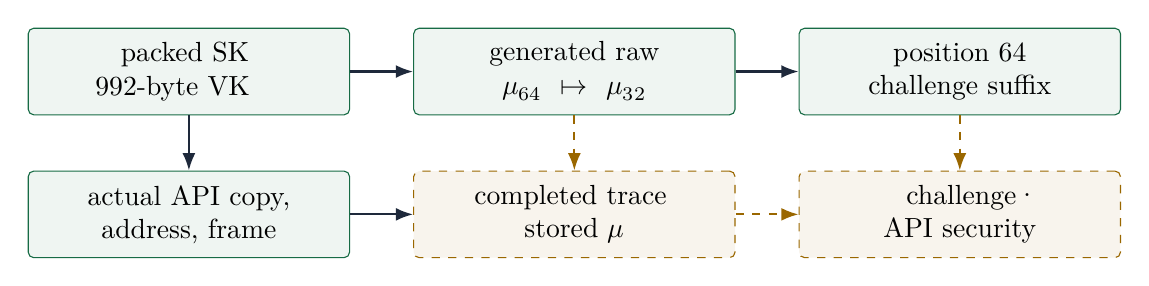
\begin{tikzpicture}[node distance=7mm and 8mm]
  \node[provennode] (kp) {packed SK의\\992-byte VK 접두부};
  \node[provennode, right=of kp] (mu) {generated raw\\\(\mu_{64}\mapsto\mu_{32}\)};
  \node[provennode, right=of mu] (chal) {position 64\\challenge suffix};
  \node[provennode, below=of kp] (api) {actual API copy,\\address, frame};
  \node[partialnode, below=of mu] (trace) {completed trace의\\stored \(\mu\)};
  \node[partialnode, below=of chal] (top) {전체 challenge·\\API security};
  \draw[flowarrow] (kp) -- (mu);
  \draw[flowarrow] (mu) -- (chal);
  \draw[flowarrow] (kp) -- (api);
  \draw[flowarrow] (api) -- (trace);
  \draw[openarrow] (mu) -- (trace);
  \draw[openarrow] (trace) -- (top);
  \draw[openarrow] (chal) -- (top);
\end{tikzpicture}
\caption{key/transcript 진행선. 실선은 닫힌 정리(theorem), 점선은 열린 승격이다.}
\label{fig:key-transcript-spine}
\end{figure}

\begin{figure}[ht]
\centering
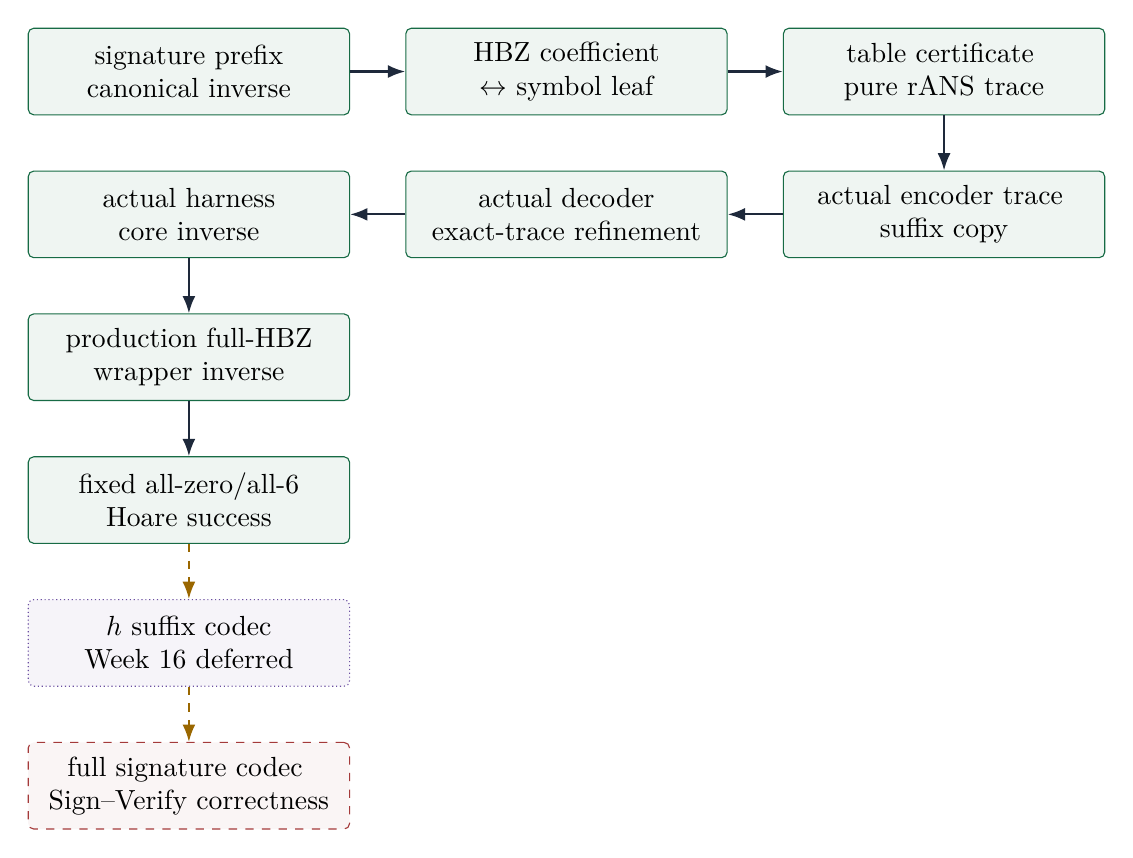
\begin{tikzpicture}[node distance=7mm and 7mm]
  \node[provennode] (prefix) {signature prefix\\canonical inverse};
  \node[provennode, right=of prefix] (leaf) {HBZ coefficient\\\(\leftrightarrow\) symbol leaf};
  \node[provennode, right=of leaf] (pure) {table certificate와\\pure rANS trace};
  \node[provennode, below=of pure] (copy) {actual encoder trace와\\suffix copy};
  \node[provennode, left=of copy] (loops) {actual decoder\\exact-trace refinement};
  \node[provennode, left=of loops] (core) {actual harness\\core inverse};
  \node[provennode, below=of core] (hbz) {production full-HBZ\\wrapper inverse};
  \node[provennode, below=of hbz] (witness) {fixed all-zero/all-6\\Hoare success};
  \node[deferrednode, below=of witness] (hcodec) {\(h\) suffix codec\\Week~16 deferred};
  \node[blockednode, below=of hcodec] (full) {full signature codec와\\Sign--Verify correctness};
  \draw[flowarrow] (prefix) -- (leaf);
  \draw[flowarrow] (leaf) -- (pure);
  \draw[flowarrow] (pure) -- (copy);
  \draw[flowarrow] (copy) -- (loops);
  \draw[flowarrow] (loops) -- (core);
  \draw[flowarrow] (core) -- (hbz);
  \draw[flowarrow] (hbz) -- (witness);
  \draw[openarrow] (witness) -- (hcodec);
  \draw[openarrow] (hcodec) -- (full);
\end{tikzpicture}
\caption{signature codec 진행선. Week~11은 actual encoder의 성공
접미부(success suffix)를, Week~12는 exact trace를 소비하는 actual decoder를,
Week~13은 actual copy를 사이에 둔 core 합성(composition)을, Week~14는
production full-HBZ wrapper 경계를, Week~15는 fixed all-6 failure exclusion을
닫았다. \(h\) codec은 Week~16 MINCORE 전환으로 동결되었다.}
\label{fig:codec-spine}
\end{figure}

\subsection{1단계: packed secret key의 검증키 몫(quotient)}

순수 배열 수준에서 술어
\[
  \operatorname{VKPrefix}_{992}(sk,vk)
  \Longleftrightarrow
  \forall,0\le i<992,\;sk_i=vk_i
\]
를 둔다. \sourcepath{PackedKeyPrefix.ec}는 다음 기본 사실을 증명한다.

\begin{itemize}
  \item 한 바이트씩 복사하는 loop invariant가 다음 index로 보존된다;
  \item 992바이트를 모두 복사하면 prefix relation이 성립한다;
  \item index 992 이후의 쓰기는 이미 완성된 접두부를 바꾸지 않는다.
\end{itemize}

이 배열 보조정리(lemma)는 실제 추출 절차로 올라간다.

\begin{verified}[실제 packer의 접두부]
\theoremname{pack_sk_m23_mode2_vk_prefix}는 mode~2 상수 아래 실제 generated
\identifier{_pack_sk_m23}가 반환할 때 결과 secret-key 배열의 첫 992바이트가
입력 verification-key 배열과 같음을 보인다. 뒤이어 eta-vector와 key를 쓰는
루프가 이 접두부를 보존한다.
\end{verified}

\begin{verified}[internal KeyGen 반환]
\theoremname{keypair_full_m23_mode2_return_prefix}와
\theoremname{keypair_internal_mode2_return_prefix}는 위 관계를 실제 generated
KeyGen 반환값까지 올린다.
\[
  \text{KeyGen returns }(vk,sk)
  \Longrightarrow \operatorname{VKPrefix}_{992}(sk,vk).
\]
\end{verified}

두 정리(theorem)는 \statusproved\ partial correctness다. KeyGen rejection loop의
종료, 전체 출력분포, 논문 KeyGen과의 동일성을 증명하지 않는다. 따라서
\claimid{FC-KG-TOP}은 여전히 \statuspartial 이다.

\subsection{2단계: 로컬 배열에서 public memory까지}

KeyGen이 반환한 배열 관계를 Sign/Verify의 실제 API 입력에 사용하려면 네 종류의
화살표가 필요하다.

\begin{enumerate}
  \item KeyGen local VK/SK 배열을 외부 주소로 복사하는 exporter;
  \item Sign이 외부 SK를 local 배열로 가져오는 importer;
  \item Verify가 외부 VK를 local 배열로 가져오는 importer;
  \item 정수 주소와 \(W64\) 주소가 같은 구간을 나타낸다는 canonical bridge.
\end{enumerate}

\sourcepath{ApiKeyMemoryBridge.ec}는 실제 copy helper에 대해 mode~2의
992/1408바이트 prefix와 disjoint frame을 증명한다.

\begin{verified}[실제 raw KeyGen의 순차 export]
\theoremname{keypair_raw_api_exports_matching_prefixes}는 실제
\identifier{cryptolab_haetae_mode2_keypair_internal}이 반환할 때, 명시적인
valid/canonical/disjoint region 계약 아래 외부 SK와 VK 구간의 첫 992바이트가
같음을 보인다.
\end{verified}

이 단계는 단순히 ``copy 함수가 복사한다''보다 강하지만 메모리 안전성 전체보다
약하다. pointer validity와 separation은 전제로 드러나며, KeyGen 종료성은
여전히 결론이 아니다.

\subsection{3단계: Sign과 Verify의 generated raw \texorpdfstring{\(\mu\)}{mu}}

Sign은 local packed SK의 접두부를 흡수하고 64바이트 \(\mu\)를 squeeze한다.
Verify는 global memory의 VK 구간을 흡수하고 32바이트를 squeeze한다. 실제
generated helper chain은 초기화, key/pre/message absorb, Keccak permutation,
finalize, squeeze를 서로 다른 절차 표면으로 실행한다.

\sourcepath{ExtractedMuHashPrefix.ec}가 leaf 관계들을 증명하고,
\sourcepath{ExactMuTopControl.ec}가 실제 top 절차로 올린다.

\begin{verified}[generated raw \(\mu\) 접두부]
명시적인 mode~2 key-prefix, 같은 pre/message 구간, raw-branch, valid/no-wrap
전제 아래
\[
  \mathsf{SignRawMu}\sim\mathsf{VerifyHashMu}
\]
가 성립하며 결론은
\[
  \take_{32}(\mu^{64}_{\mathrm{Sign}})
  =\mu^{32}_{\mathrm{Verify}}
\]
이다. 명명된 정리(theorem)는
\theoremname{sign_verify_generated_raw_mu_prefix}다.
\end{verified}

이 정리(theorem)는 두 실제 generated 절차를 theorem surface에 직접 둔다.
wrapper에 대한 추상 명제(abstract proposition)를 실제 절차와 동일시해 버린
것이 아니다. 또한
\theoremname{raw_prelen_shr63_zero}와
\theoremname{raw_prelen_branch_guard}가 실제 bit-level 분기로 raw 경로를
선택함을 보인다.

\subsection{4단계: 전체 메모리 등식(whole-memory equality)에서
read-region 등식(read-region equality)으로}

실제 Sign이 signature를 출력한 뒤에는 두 실행의 global memory 전체가 같을
이유가 없다. 필요한 것은 hash가 읽는 key, pre, message 구간뿐이다.

\begin{verified}[region-local generated hash]
\theoremname{sign_verify_generated_raw_mu_prefix_regionwise}는 서로 다른 global
memory를 허용한다. key/pre/message read region이 점별로 관련되면 실제
generated Sign/Verify raw hash 반환값이 같은 32바이트 접두부를 갖는다.
\end{verified}

\begin{verified}[Sign 출력 frame]
\theoremname{sign_raw_api_frames_reused_regions}는 실제 raw Sign이 signature
1474바이트와 siglen 8바이트를 쓰더라도, 출력 구간과 분리된 VK/SK/pre/message
구간을 보존함을 보인다.
\end{verified}

두 정리(theorem)를 합치면 ``Sign 뒤에도 Verify가 읽을 입력 바이트가 남아 있다''는
memory-level 기반이 생긴다. 하지만 완료된 두 trace가 저장한 \(\mu\)를 직접
비교하는 마지막 운송은 아직 열려 있다. 이는 \cref{sec:boundaries}에서
분리한다.

\subsection{5단계: position~64 challenge suffix}

Sign과 Verify가 같은 challenge state와 position을 갖고 position이 64이며,
앞 단계에서 얻은 \(\mu_{32}\)가 같다고 하자. 실제 generated absorb helper를
한 번씩 실행한 뒤 상태와 position이 같다는 정리(theorem)가 있다.

\begin{verified}[국소 challenge-suffix zero-loss]
\theoremname{generated_raw_mu_to_challenge_suffix_zero_loss}는 실제 generated
raw \(\mu\) 절차와 실제 generated 32-byte challenge absorb helper를 각 변에
연속 호출한다. 명시된 전제 아래 최종 \((\mathit{state},\mathit{position})\)이
같다.
\end{verified}

따라서 raw/internal generated seam에서는 deterministic loss가 0이다. 하지만
이 정리(theorem)는 highbits/LSB prefix, 전체 challenge, 실제 accepted API trace의 stored
\(\mu\), context branch를 포함하지 않는다.

\subsection{6단계: 실제 caller의 control과 accepted Verify}

Week~4--6은 위 leaf 결과를 실제 public/raw caller 문맥에 배치하는 작업을 했다.
현재 다음이 각각 컴파일된다.

\begin{itemize}
  \item 실제 raw Sign의 exact \(\mu\) trace와 hash input binding;
  \item 실제 raw/cryptolab Verify의 모든 early-reject/tail branch를 보존하는
        exact trace;
  \item Verify가 accept하면 실제 tail과 hash call에 도달한다는 방향;
  \item accepted Verify가 실제 VK/pre/message descriptor를 사용했다는 binding;
  \item 실제 Sign 다음 실제 Verify를 순차 실행하는 exact trace;
  \item 그 순차 실행 동안 key/pre/message 구간을 보존하는 frame.
\end{itemize}

\begin{verified}[accept에서 tail로]
\[
  \mathit{VerifyResult}=0
  \Longrightarrow \mathit{tail\_reached}
\]
가 실제 raw/cryptolab Verify에 대해 증명되었다. 역방향도 아니고,
``임의의 1474바이트 signature가 tail에 도달한다''는 명제(proposition)도 아니다.
\end{verified}

\begin{verified}[실제 sequential trace]
\theoremname{raw_sign_then_verify_actual_exact_trace}는 실제 raw Sign 후 실제 raw
Verify의 반환값과 최종 메모리를 두 instrumented trace의 순차 실행과 맞춘다.
\end{verified}

그럼에도 \claimid{OBL-DIRECT-OBSERVED-MU}는 \statuspartial 이다. exact trace는
관측 위치와 값을 노출하지만, 별도의 pRHL 반환값 정리(theorem)를 이미 종료한 두 trace의
ghost field 등식(equality)으로 자동 운반하지 않는다.

\subsection{7단계: 실제 signature prefix의 section--retraction}

\sourcepath{Mode2SignaturePrefixPack.ec}와
\sourcepath{Mode2SignaturePrefixUnpack.ec}는 실제 generated prefix loop의
정확한 layout을 연다. 두 절차를 실제 순서로 호출하는 harness가
\sourcepath{Mode2SignaturePrefixRoundTrip.ec}에 있다.

\begin{verified}[mode~2 prefix round trip]
canonical challenge와 canonical signed-low 입력에 대해
\theoremname{pack_unpack_sig_prefix_mode2_roundtrip}은
\begin{align*}
  \mathit{decodedChallenge}[0..256)&=\mathit{challenge}[0..256),\\
  \mathit{decodedLow}[0..1024)&=\mathit{low}[0..1024)
\end{align*}
를 보이고, decoded-low의 사용하지 않는 tail도 frame한다.
\end{verified}

정준 전제(canonical premise)의 all-zero witness도 컴파일되어
명제(proposition)가 공허하지
않다. 그러나 결과는
서명 앞 1056바이트뿐이다. metadata 두 바이트와 416바이트 suffix, padding,
전체 unpack 성공은 포함되지 않는다.

\subsection{8단계: HBZ coefficient--symbol leaf}

HBZ 입력은 1024개 coefficient \(h_i\in[-6,7)\)다. prepare는
\(s_i=h_i+6\in\{0,\ldots,12\}\)을 계산하고, apply는 \(s_i-6\)을 32비트
word 표현으로 복원한다.

\begin{verified}[HBZ leaf inverse]
\theoremname{encode_prepare_decode_apply_mode2_inverse}는 canonical HBZ 배열에
대해 실제 prepare와 실제 apply 절차를 순차 실행하면 앞 1024개 coefficient가
복원되고, decoder coefficient tail이 보존되며, prepare의 \(bad\) 출력이 0임을
보인다.
\end{verified}

이 정리(theorem)는 rANS core를 건너뛴 leaf-level inverse다. 따라서 이것만으로 실제
compressed suffix가 round trip한다고 말할 수 없다.

\subsection{9단계: 실제 표와 순수 rANS 수학}

mode~2 HBZ의 13개 frequency는 합이 1024이고, 누적구간은
\([0,1024)\)를 분할(partition)한다. \sourcepath{Mode2HbzTableCertificate.ec}는 이
산술뿐 아니라 reciprocal/bias와 packed decoder word의 의미를 증명한다.
생성된 실제 literal array가 그 certificate를 만족한다는 정리(theorem)도 별도 파일에서
컴파일된다.

\begin{verified}[순수 단일 단계 역함수(inverse function)]
각 symbol \(s\)와 허용된 state \(x\)에 대해 실제 table에서 얻은
\(c_s,f_s\)를 사용하면
\[
  D_s(E_s(x))=x
\]
이고, reciprocal을 쓰는 fast encoder step도 명시된 normalized range에서
수학적 \(E_s\)와 같다.
\end{verified}

Week~9은 단일 단계 사이의 normalization byte를 포함하는 순수
\(xs/cuts/bytes\) trace를 정의했다.

\begin{verified}[순수 byte-stack]
canonical symbol list에 대해 다음이 컴파일된다.
\begin{itemize}
  \item normalization은 매 단계 0, 1, 2바이트만 방출한다;
  \item 방출된 segment를 decoder 순서로 append하면 원래 state를 복원한다;
  \item 4-byte little-endian 초기 state는 parse 뒤 복원된다;
  \item 모든 trace state는 \([2^{23},2^{31})\)에 머문다;
  \item trace의 head symbol, reduced state, normalization segment가 한 단계씩
        decode된다.
\end{itemize}
\end{verified}

\begin{verified}[실제 copy와 control harness]
\theoremname{copy_encoded_suffix_correct}는 actual
\identifier{__copy_encoded_suffix}의 점별 slice copy와 tail frame을 보인다.
\theoremname{actual_rans_harness_branches_on_encoder_result}는 실제 encoder,
실제 copy, 실제 decoder를 이 순서로 호출하고 encoder의 실제 \(bad\) 결과가
0일 때 정확히 decoder를 실행하며 \((count,size,m)=(1024,\mathit{size},13)\)을
전달함을 보인다.
\end{verified}

이 control 정리(theorem) 자체는 decoder success, symbol equality, 최종 state,
소비 byte 수를 결론내리지 않는다. Week~12의 별도 decoder 정리(theorem)가
exact-trace 입력 관계(input relation) 아래에서 그 의미론(semantics)을 증명하지만,
이 시점에는 아직 control harness 안에 합성되지 않았다. Week~13의
\theoremname{actual_rans_encode_copy_decode_inverse}가 같은 harness에 그
의미론적 결론(semantic conclusion)을 추가한다.

\subsection{10단계: actual encoder의 국소 의미론(local semantics)}

Week~10에는 rANS encoder를 위한 \WeekTenTargetCount 개 타깃이 authored target
manifest에 편입되어 fresh compile되었다. 이들은 순수 trace와 실제 생성 절차
사이의 한 거대한 정리(theorem)를 바로 선언하지 않고, 배열(array)--리스트(list),
word 산술(word arithmetic), 내부 정규화(inner normalization), 최종 직렬화(final
serialization)를 분리한다 \cite{week10-report,rans-encoder-invariant}.

\begin{verified}[배열(array), word, 직렬화(serialization) 보조정리(lemmas)]
\theoremname{encode_trace_suffix_extension}은 실제 1024-byte 기호 배열(symbol
array)의 접미부(suffix)를 한 기호씩 확장하는 순수 trace 점화식(recurrence)으로
옮긴다. \theoremname{actual_mode2_encoder_word_step_correct}는 literal table의
reciprocal, shift, bias, complement를 쓰는 실제 word 식이 순수 fast step과 같음을
보인다. \theoremname{actual_encoder_final_state_serialization}은 네 번의
\identifier{set8}이 32-bit state의 little-endian 직렬화(serialization)와 같음을
보인다.
\end{verified}

\begin{verified}[실제 내부 루프(inner loop)와 성공 크기(success size)]
\theoremname{actual_rans_encode_inner_no_underflow}는 실제 generated
\identifier{_rans_encode}의 중첩 정규화 루프(nested normalization loop)에
바이트 구간(byte segment)과 접두부 프레임(prefix frame) 불변식(invariant)을
설치하여 \(W64\) cursor 비언더플로(no-underflow)를 보인다.
\theoremname{actual_rans_encode_success_size_bound}는 같은 절차가 반환한다면
\[
  bad\ne0\quad\lor\quad
  \bigl(bad=0\land 0\le off\le1020\land
        4\le1024-off\le1024\bigr)
\]
임을 보이는 실제 부분정확성(actual partial correctness) 정리(theorem)다.
\end{verified}

Week~10 단계의 끝에서 이 결과는 이전의 \(bad\in\{0,1\}\) 제어
정리(control theorem)보다 강했지만, actual 반환 접미부(returned suffix) 전체가
\(
\operatorname{TraceBytes}
  (\operatorname{SymbolList}(symbols_0))
\)
와 같다는 명제(proposition)는 아니었다. 당시 내부 phase는 보수적인 \(0..4\)
범위(range)를 사용했고, 실제 바깥 반복(outer iteration)의 한 기호
상태전이(state transition)와 마지막 네 store의 절차 수준 합성이 열려 있었다.

\subsection{11단계: actual encoder의 전역 trace closure}

Week~11은 \WeekElevenTargetCount 개 encoder 타깃을 추가하여 Week~10의 국소
전이(local transition)를 전체 성공 출력(global success output)으로 합성했다
\cite{week11-report,rans-encoder-invariant}. 핵심 불변식(invariant)은 임의의
inner-loop 시작 배열이 아니라 최초 배열 \(enc_0\)와 이미 처리한 순수
접미부(pure suffix)를 함께 기억한다.

\begin{verified}[tail-aware 불변식(invariant)과 생성 산술(generated arithmetic)]
\identifier{encoder_inner_tail_inv} 명제(proposition)는 actual inner loop가
\[
  \operatorname{InnerWrittenSuffix}(x_0,s,k)
  \mathbin{+\!\!+}\operatorname{EncodeTrace}(tail).bytes
\]
를 현재 cursor 뒤에 보존한다고 표현한다.
\theoremname{encoder_inner_tail_exit_exact} 보조정리(lemma)는 실제 guard가
끝나면 \(k=\operatorname{NormalizationLen}(x_0,s)\le2\)임을 회복한다.
\theoremname{generated_loaded_nested_word_update} 보조정리(lemma)는 실제 table
load, reciprocal high product, shift, complement와 bias를 순수 fast step으로
운송한다.
\end{verified}

\begin{verified}[encoder trace closure 정리(theorem)]
\theoremname{actual_rans_encode_trace_closure}는 실제 generated
\identifier{RansEncodeTarget.M._rans_encode}를 직접 열어, 반환한다면 실패하거나
성공 시
\[
\begin{gathered}
  bad'=0,\qquad 0\le off'\le1020,\qquad
  4\le1024-off'\le1024,\\
  \operatorname{SegmentMatches}
    \bigl(enc',off',
      \operatorname{TraceBytes}(\operatorname{SymbolList}(symbols_0))\bigr),\\
  off'+\left|
    \operatorname{TraceBytes}(\operatorname{SymbolList}(symbols_0))
  \right|=1024,\qquad
  \operatorname{PrefixFrame}(enc_0,enc',off')
\end{gathered}
\]
가 모두 성립함을 보인다.
\theoremname{actual_rans_encode_trace_refinement}는 같은 결론을 부모
refinement 표면에 전개한 따름정리(corollary)다.
\end{verified}

마지막 네 generated store가 직렬화된 상태(serialized state)를 누적
normalization suffix 앞에 붙인다는 합성도 이 정리(theorem) 안에 들어간다.
따라서 \claimid{OBL-RANS-ACTUAL-INNER-NORMALIZE},
\claimid{OBL-RANS-FINAL-SERIALIZATION},
\claimid{OBL-RANS-ENCODE-REFINEMENT}는 각각 명시된 범위에서 \statusproved 다.
그러나 이는 Hoare 부분정확성(Hoare partial correctness)이다. 실제 호출의
종료성(termination)이나 \(bad'=0\)인 실행의 존재를 주지 않으므로
이 정리 하나만으로는 고정 입력의 성공을 결론낼 수 없다. Week~11 당시
\claimid{OBL-RANS-ACTUAL-SUCCESS-WITNESS}는 \statuspartial 이었고, Week~15의
별도 all-6 정리가 반환하는 fixed-input 실행에서 failure를 배제한다.

\subsection{12단계: actual decoder의 exact-trace 의미론(semantics)}

Week~12는 \WeekTwelveTargetCount 개 decoder 타깃을 추가하여 순수 trace의
좌표(coordinates)를 actual generated decoder의 두 중첩 반복(nested loops)에
설치했다 \cite{week12-report,rans-decoder-invariant}. 핵심 입력 술어(input predicate)
\identifier{actual_mode2_decoder_trace_input}은 임의의 buffer가 아니라 다음을
동시에 요구한다.

\begin{itemize}
  \item expected symbol array가 mode~2 정준 기호열(canonical symbol stream)임;
  \item \(encoded\_size=|\operatorname{TraceBytes}
        (\operatorname{SymbolList}(expected))|\)이고 \(4\le encoded\_size\le1024\);
  \item \(buffer_0[0..encoded\_size)\)가 그 exact trace와 점별로 일치함;
  \item generated normalization read마다 pure trace segment의 해당 byte를 읽음;
  \item actual state fields가 \((count,size,m)=(1024,encoded\_size,13)\)임;
  \item 실제 mode~2 \identifier{symbol_words}와 \identifier{dsyms_words}를 사용함.
\end{itemize}

\begin{verified}[decoder trace 좌표(coordinates)와 불변식(invariant)]
\identifier{decoder_state_at}, \identifier{decoder_cursor},
\identifier{decoder_segment_at}은 순수 \(xs/cuts/bytes\) trace의 상태(state),
cursor, normalization segment를 iteration별 좌표로 만든다.
\identifier{decoder_outer_trace_live} 명제(proposition)는
\[
  x=\operatorname{DecoderStateAt}(i),\qquad
  off=\operatorname{DecoderCursor}(i)
\]
와 decoded prefix의 등식(equality), untouched tail frame을 함께 보존한다.
안쪽 불변식(inner invariant)은 해당 segment를 정확히 0/1/2-byte replay하고 다음
순수 상태(pure state)를 복원한다.
\end{verified}

\begin{verified}[actual decoder exact-trace 정리(theorem)]
\theoremname{actual_rans_decode_trace_refinement}는 실제 generated
\identifier{RansDecodeTarget.M._rans_decode}를 직접 열어, 반환한다면
\[
\begin{gathered}
  bad'=0,\qquad off'=encoded\_size,\\
  \forall i,\;0\le i<1024\Longrightarrow decoded'_i=expected_i,\\
  \forall i,\;1024\le i<2048\Longrightarrow decoded'_i=decoded_{0,i}
\end{gathered}
\]
를 보인다. 내부 종료 상태(internal exit state) \(x=2^{23}\)도 유도하여 실제 final
reject를 통과시키지만, generated ABI는 이 \(x\)를 반환하지 않으므로 반환
배열(returned array)과 state fields만 사후조건(postcondition)에 공개된다.
\end{verified}

따라서 \claimid{OBL-RANS-DEC-NORMALIZE}와
\claimid{OBL-RANS-DECODE-REFINEMENT}는 exact-trace Hoare
부분정확성(Hoare partial correctness)으로 \statusproved 다. Week~12 종료
시점에는 encoder의 \identifier{segment_matches}와 actual copy의
\identifier{slice_eq}를 위 입력 술어(input predicate)로 운송하는 sequential
harness 정리(theorem)가 없었다. Week~13의 다음 단계가 정확히 이 간선(edge)을
닫는다.

\subsection{13단계: actual encoder--copy--decoder core 역함수(inverse function)}

Week~13은 \WeekThirteenTargetCount 개 타깃을 추가하여 실제
\identifier{Mode2RansActualHarness.run}의 세 호출을 순서대로 합성했다
\cite{week13-report,rans-core-composition}. 이 harness와 control 정리(theorem)는
\sourcepath{Mode2RansActualInverse.ec}에 있고, 의미론적 closure는
\sourcepath{Mode2RansCoreCompositionBridge.ec}와
\sourcepath{Mode2RansCoreActualInverse.ec}에 분리되어 있다. 새 bridge 파일은 다음
운송 보조정리(transport lemmas)를 제공한다.

\begin{itemize}
  \item \theoremname{copied_suffix_is_exact_trace}: encoder의
        \identifier{segment_matches}와 actual copy의 \identifier{slice_eq}에서
        copied buffer의 offset~0 exact trace를 얻음;
  \item \theoremname{trace_bytes_trace_segment_nth}: 전역
        \identifier{trace_bytes} 좌표를 symbol별 local segment와 decoder cursor
        좌표로 분해함;
  \item \theoremname{segment_matches_implies_exact_decoder_segment_input}:
        global trace 구간(segment)에서 decoder의 모든 pointwise byte-read 전제를
        얻고, \theoremname{segment_matches_implies_decoder_word_reads}가 이를 actual
        W64 read 형태로 옮김;
  \item \theoremname{actual_decoder_input_from_copied_trace}와
        \theoremname{configured_decoder_state_fields}: copied trace와 실제 세 state
        store를 각각 decoder 입력 관계(input relation)의 구성요소로 만듦;
  \item \theoremname{actual_decoder_input_from_configured_trace}: copied trace,
        정준 기호열(canonical symbol stream), size bound, 실제 세 state store에서
        Week~12 decoder 입력 술어(input predicate) 전체를 구성함;
  \item \theoremname{encoder_success_size_word_bridge}: actual (W64) 뺄셈과
        정수 trace 크기(integer trace size)를 no-wrap 범위에서 동일시함.
\end{itemize}

\begin{verified}[\claimid{OBL-RANS-CORE-INVERSE}]
\theoremname{actual_rans_encode_copy_decode_inverse}의 의미론적 전제(semantic
precondition)는 harness argument binding과
\identifier{mode2_hbz_symbol_stream}뿐이다. encoder 성공, copied-trace 등식,
decoder 실행 또는 성공을 전제로 요구하지 않는다. 반환한다면 다음 두 가지(branch)
중 하나다.
\[
\begin{aligned}
\mathsf{failure}:\quad
  &encoderBad\ne0,\quad \neg decoderRan,\quad decoderOff=0,\quad decoderBad=1,\\
  &decoded'=decoded_0,\quad decoderState'=decoderState_0;\\[0.3em]
\mathsf{success}:\quad
  &encoderBad=0,\quad decoderRan,\quad (count,size,m)=(1024,encodedSize,13),\\
  &decoderBad=0,\quad decoderOff=encodedSize,\\
  &decoded'[0..1024)=expected[0..1024),\\
  &decoded'[1024..2048)=decoded_0[1024..2048).
\end{aligned}
\]
성공 가지(success branch)는 actual encoder suffix relation과 초기 prefix frame도
보존한다. 따라서 세 actual generated 절차의 core 역함수(inverse function)가 성공
조건부 부분정확성(success-conditioned partial correctness)으로 컴파일된다.
\end{verified}

\theoremname{core_composition_preconditions_satisfiable}는 all-zero 정준 기호
배열(canonical symbol array)로 전제의 비공허성(non-vacuity)만 보인다. 결론이
실패/성공의 합(disjunction)이므로 실제 성공 가지의 도달가능성(reachability)이나
encoder/decoder 종료성(termination)은 따라오지 않는다. 따라서
Week~13 시점에는 \claimid{OBL-RANS-ACTUAL-SUCCESS-WITNESS}가
\statuspartial 로 남았다. 이 결론만으로는 production full-HBZ wrapper까지 자동
승격되지 않았고, 별도 승격은 Week~14에, fixed all-6 failure exclusion은
Week~15에 각각 닫혔다.

\subsection{14단계: production full-HBZ wrapper 경계}

Week~14는 \WeekFourteenTargetCount 개 타깃을 추가해 focused full-HBZ 절차와
실제 SignaturePack/Unpack 추출 경계를 연결했다
\cite{week14-report,hbz-full-wrapper-composition}. 증명 사슬은 다음 네 층이다.

\begin{enumerate}
  \item \sourcepath{Mode2HbzInternalBoundaries.ec}는 focused full wrapper 내부의
        prepare, rANS encode/decode, apply 호출을 기존 actual 정리(theorem)에
        exact하게 연결한다.
  \item \theoremname{actual_encode_hb_z1_full_mode2_trace}는 canonical HBZ
        coefficient를 받는 실제 full encoder의 실패/성공 분기를 보존하고, 성공
        시 prepared symbol witness, 정확한 trace size/segment와 suffix frame을 준다.
  \item \theoremname{actual_decode_hb_z1_full_mode2_inverse}는 그 exact trace와
        prepared-symbol 관계에서 실제 full decoder가 \(bad=0\), 원래 1024개
        coefficient prefix와 coefficient tail frame을 반환함을 보인다.
  \item \theoremname{actual_hbz_full_encode_decode_inverse_mode2}가 focused
        encode/decode harness를 합성하고,
        \theoremname{signature_pack_unpack_hbz_full_actual_exact}가 이를 production
        SignaturePack/Unpack harness와 결과 tuple 및 \identifier{decoder_ran}까지
        exact하게 맞춘다.
\end{enumerate}

\begin{verified}[\claimid{OBL-SIG-HBZ-ENCODE-DECODE}]
Hoare 따름정리(corollary)
\theoremname{signature_pack_unpack_hbz_full_inverse_mode2}의 유일한 의미론적
사전조건(semantic precondition)은 argument binding과
\identifier{canonical_hbz_mode2}다. 반환한다면 다음 합(disjunction)이 성립한다.
\[
\begin{aligned}
\mathsf{failure}:\quad
  &size=0,\quad \neg decoderRan,\quad encoded=out_0,\\
  &decoded=decoded_0,\quad bad=bad_0;\\[0.3em]
\mathsf{success}:\quad
  &size\ne0,\quad 4\le size\le1024,\quad decoderRan,\quad bad=0,\\
  &decoded[0..1024)=hbz_0[0..1024),\\
  &\operatorname{CoeffTailFrame}(decoded_0,decoded),\quad
    \operatorname{SuffixFrame}(out_0,encoded),
\end{aligned}
\]
그리고 성공 가지에는 prepared-symbol witness와 그
\identifier{mode2_trace_bytes}에 대한 \identifier{segment_matches}가 존재한다.
따라서 production wrapper 합성은 성공 조건부 부분정확성(success-conditioned
partial correctness)으로 \statusproved 다.
\end{verified}

이 정리(theorem)는 encoder 성공을 전제로 받지 않고 실제 실패 branch를 보존한다.
그러나 canonical all-zero HBZ 입력이 actual encoder의 nonzero-size branch에
들어가는 반환 실행의 failure exclusion이나 encoder/decoder 종료성은 이
Week~14 정리 자체가 증명하지 않는다. prepare 뒤의 해당 symbol stream이
all-6이라는 사실과 실제 encoder의 성공은 서로 다른 명제다. 전자는
Week~15의 별도 budget/failure-cause 정리와 합성되지만, 종료성은 여전히 별도다.

\subsection{15단계: fixed all-6 actual success 사후조건}

Week~15는 \WeekFifteenTargetCount 개 타깃을 추가하여
\claimid{OBL-RANS-ACTUAL-SUCCESS-WITNESS}를 fixed-input Hoare
부분정확성(partial correctness)으로 닫았다
\cite{week15-report,rans-actual-success-witness}. 첫 타깃
\sourcepath{Mode2RansAllSixBudget.ec}는 다음 순수·prepare 사슬을 증명한다.

\begin{itemize}
  \item \theoremname{zero_hbz_get32}, \theoremname{zero_hbz_canonical}과
        \theoremname{actual_prepare_zero_hbz_all_six}가 실제 prepare 반환의
        \(bad=0\)과 1024개 all-6 prefix를 산출함;
  \item \theoremname{symbol6_normalization_len_le1}가 symbol~6의 각 step이
        normalization byte를 최대 하나만 방출함;
  \item \theoremname{all_six_first_four_no_normalization}과
        \theoremname{all_six_normalization_budget}이 첫 네 step의 0-byte와
        전체 1020-byte 상계를 결합함;
  \item \theoremname{all_six_trace_fits_mode2}가 마지막 state 네 바이트를 더해
        total trace size를 \([4,1024]\)에 둠.
\end{itemize}

기존 encoder closure는
\theoremname{actual_rans_encode_failure_trace_cause}로 강화되어 nonzero
\(bad\)이면 normalization trace가 1020바이트를 넘는다고 결론낸다. all-6
상계와 모순시키면 다음 실제 사후조건을 얻는다.

\begin{verified}[\claimid{OBL-RANS-ACTUAL-SUCCESS-WITNESS}]
\theoremname{actual_rans_encode_all_six_success}는 actual
\identifier{_rans_encode}의 모든 반환 실행에서 \(bad=0\),
\(0\le off\le1020\), \(4\le1024-off\le1024\), exact trace segment와 prefix
frame을 준다. \theoremname{actual_encode_hb_z1_full_zero_success}와
\theoremname{signature_pack_hbz_zero_success_mode2}가 이를 focused/production
full encoder로 올리고,
\theoremname{signature_pack_unpack_hbz_zero_success_mode2}가 production zero
round trip, \identifier{decoder_ran}, decoder \(bad=0\), coefficient/encoded
tail frame을 결론낸다.
\end{verified}

이 증명은 success를 사전조건으로 요구하지 않지만 Hoare 논리의
부분정확성이다. 실제 fixed-input 실행이 종료하거나 존재한다는 명제,
losslessness, probability-one success 또는 \identifier{phoare} 정리는 포함하지
않는다. 따라서 ``fixed all-6 Hoare success가 \statusproved''와 ``fixed-input
termination은 미증명''을 동시에 유지해야 한다.

\subsection{16단계: actual KeyGen snapshot과 KG--NTT 중단 경계}

Week~16은 \WeekSixteenTargetCount 개 KeyGen 타깃을 추가했다
\cite{week16-mincore-plan,week16-kg-report,week16-kg-ntt-mul-report}. 순수 파일
\sourcepath{Mode2KeygenSnapshot}%
\allowbreak\sourcepath{Algebra.ec}의
\theoremname{snapshot_residue_exact_low_high},
\theoremname{raw_sum_raw_residue_congruent_mod_2q},
\theoremname{snapshot_expression_from_product_congruent_mod_2q}는 canonical
residue의 low/high 분해와 doubled congruence를 증명한다.

\sourcepath{Mode2KeygenCoreEquation.ec}의 투명한
\identifier{ActualM23MatrixFinalizeSnapshot.run}은 실제
\identifier{_kp_m23_matrix(2,3)} 반환을 snapshot한 뒤 실제
\identifier{_keypair_finalize_m23(512)}를 호출한다.

\begin{verified}[actual snapshot/finalizer 경계]
\theoremname{actual_m23_matrix_finalize_snapshot}은 matrix output/NTT
representation, exact finalization과 tail frame을 합성한다. 가장 강한 정리
\theoremname{actual_m23_matrix_finalize_semantic_snapshot}은 여기에
\theoremname{finalize_semantic_output_low_high_decomposition}, HAETAE finalizer
semantics와 \theoremname{finalize_semantic_output_snapshot_mod2q_zero}를 더해,
active coefficient마다 KG-2-like 분해, adjusted \(s_2\)와 snapshot-only
mod-\(2q\) 영 합동식을 준다.
\end{verified}

세 번째 타깃 \sourcepath{Mode2KeygenNttMulBridge.ec}는 actual loop를 복제하지
않고 기존 NTT 사슬의 마지막 sound rewrite만 고정한다.
\theoremname{output_row_from_mode2_ntt_words}는 transformed-secret 표현 아래
\identifier{output_row}가
\[
  \operatorname{array256\_mont}
  \bigl(\operatorname{full\_invntt}
    (\operatorname{pointwise\_row\_words}(m,v,row))\bigr)
\]
와 정확히 같음을 증명한다.
\theoremname{output_row_repr_from_mode2_ntt_words}는 이 등식을 기존
\identifier{wide_slice_repr_bound} 계약으로 운송한다.
\theoremname{actual_m23_matrix_snapshot_rows_explicit}는 strongest snapshot
정리를 consequence로 재사용하여 두 active row 모두를 해당
full-invNTT/pointwise-word 표현으로 내린다. 어느 정리도 native \(R_q\) 곱,
보안 모형 곱 또는 원하는 KeyGen 식을 전제로 넣지 않는다.

\begin{openobligation}[\claimid{OBL-MINCORE-KEYGEN}: \identifier{STOP-KG-NTT}]
마지막 NTT-word rewrite까지는 컴파일되었지만, actual pointwise/inverse-NTT
표현을 native \(R_q\) negacyclic 곱으로 바꾸는 odd-root orthogonality/full-NTT
convolution 정리와 \identifier{Rq.poly}를 보안 모형의 integer-list 곱으로 옮기는
어댑터가 없다. 따라서 해당 행 곱
\(\sum_j A_{\mathrm{gen},ij}s_{\mathrm{gen},j}\)을 얻지 못한다. faithful KG-1,
KG-3, complete KG-4와 논문식 \(A s=qj\pmod{2q}\)는 증명되지 않았다.
\end{openobligation}

KG-NTT-MUL 감사는 이 두 누락 leaf를 특정하고 \CurrentGate 로 종료했다.
\identifier{GO-KG}가 아니며, KeyGen은 KG-2/finalization 경계에서 동결되었다.
sampler, retry, packing, public API, KeyGen 종료성과 보안은 이 actual two-call
snapshot 정리의 결론 밖에 있다. 활성 MINCORE lane은 아직
\statusspecified 인 accepted Sign core로 이동했다.

\subsection{닫힌 사슬의 정확한 끝점}

\begin{longtable}{@{}L{100mm} L{55mm}@{}}
\toprule
사슬 & 끝점 \\
\midrule
\endfirsthead
\toprule
사슬 & 끝점 \\
\midrule
\endhead
packed key \(\to\) generated raw \(\mu\) \(\to\) position-64 absorb &
\statusproved\ (raw/internal, 국소) \\
actual KeyGen export, Sign/Verify import, address/frame/control &
\statusproved\ (각 명명된 계약) \\
completed actual traces의 stored \(\mu\) 직접 등식(direct equality) &
\statuspartial \\
canonical signature prefix round trip &
\statusproved\ (1056-byte prefix) \\
HBZ leaf, table, pure rANS step와 byte trace &
\statusproved\ (순수/leaf) \\
actual encoder array/list·word·serialization leaf &
\statusproved\ (Week~10 국소 명제(local propositions)) \\
actual encoder 내부 byte/frame와 성공 크기 &
\statusproved\ (exact \(0..2\), actual partial correctness) \\
actual encoder 전체 접미부(trace suffix) refinement &
\statusproved\ (성공 조건부 부분정확성(success-conditioned partial correctness)) \\
actual decoder exact-trace refinement &
\statusproved\ (1024-symbol 복원, exact consumption, tail frame) \\
actual encoder--copy--decoder harness control &
\statusproved\ (호출·분기만) \\
actual encoder--copy--decoder의 inverse &
\statusproved\ (성공 조건부 부분정확성(success-conditioned partial correctness)) \\
production full-HBZ wrapper inverse &
\statusproved\ (success-conditioned partial correctness, production boundary) \\
actual encoder success witness &
\statusproved\ (fixed all-6 입력의 Hoare failure exclusion; 종료성/losslessness 없음) \\
actual KeyGen matrix/finalize snapshot &
\statuspartial\ (KG-2-like 분해와 snapshot 합동식은 증명;
마지막 NTT-word rewrite 뒤 \identifier{STOP-KG-NTT}) \\
\(h\) suffix codec &
\statusdeferred\ (Week~16 MINCORE KeyGen 범위) \\
full signature codec와 Sign--Verify correctness &
\statusblocked \\
구현 수준 기능정확성과 보안 &
\statusspecified / \statuspartial \\
\bottomrule
\end{longtable}

\section{HBZ/rANS 동역학계와 fixed-input failure exclusion}
\label{sec:rans-frontier}

\subsection{왜 success 사후조건과 종료성은 다른 주장인가}

signature prefix의 역함수(inverse function), HBZ coefficient--symbol leaf,
그리고 actual encoder가 정준 기호열(canonical symbol stream)을 순수 byte
trace로 보내는 간선(edge), exact trace를 actual decoder가 정준 기호열로
되돌리는 간선(edge), actual copy를 사이에 둔 core 합성(composition), 그리고
production SignaturePack/Unpack의 full-HBZ wrapper 경계는 각각 닫혔다.
Week~15는 canonical all-zero HBZ가 만드는 all-6 stream에서 반환하는 actual
encoder의 failure를 배제하고 production zero round trip까지 올렸다
\cite{week15-report,rans-actual-success-witness}. 따라서
\claimid{OBL-RANS-ACTUAL-SUCCESS-WITNESS}는 fixed-input Hoare
부분정확성(partial correctness)으로 \statusproved 다. 다만 반환·실행 존재를
보장하는 termination/losslessness 정리는 아니다. 이 결과 이후 프로젝트는
Week~16 KeyGen/Sign을 거쳐 현재 \CurrentGate 로 이동했다.

rANS 자체의 정수 산술(integer arithmetic)은 복잡하지 않다. 어려움은 encoder가
symbol을 뒤에서부터
읽고 byte buffer cursor를 감소시키는 반면, decoder는 복사된 buffer를 앞에서부터
읽는다는 구현 방향성에 있다. 순수 역함수 정리(pure inverse-function theorem)를
실제 두 중첩 loop의 state와 결합하는 불변식(invariant)이 핵심이다. Week~11은
reverse encoder 쪽 결합을, Week~12는 forward decoder 쪽 결합을, Week~13은
두 정리(theorem) 사이의 actual copy와 전제 운송(premise transport)을 완료했다.
Week~14는 이 core 정리(theorem)를 production
\identifier{_encode_hb_z1_full}/\identifier{_decode_hb_z1_full}의
prepare/apply·frame·size 의미론(semantics)과 합성했다. Week~15는 actual prepare가
all-6 stream을 만든다는 사실, 1020-byte normalization budget, actual failure의
필요조건을 합성해 반환하는 fixed input 실행의 nonzero-size branch를 강제한다.
HBZ에 남은 간극(gap)은 이 실행 자체의 종료·존재, 임의의 canonical 입력에 대한
전역 성공, malformed rejection과 probabilistic losslessness다.

\subsection{13-symbol 분할(partition)}

HBZ 정준 계수(canonical coefficient) \(h_i\in[-6,7)\)를
\(s_i=h_i+6\)으로 옮기면 alphabet은
\[
  \Sigma=\{0,1,\ldots,12\}
\]
이다. rANS scale을 \(M=1024\)라 하고 각 symbol의 누적 시작점과
빈도(frequency)를
\[
\begin{aligned}
(c_s)_{s=0}^{12}
  &=(0,1,2,3,8,66,312,710,957,1016,1021,1022,1023),\\
(f_s)_{s=0}^{12}
  &=(1,1,1,5,58,246,398,247,59,5,1,1,1)
\end{aligned}
\]
로 둔다. certificate는
\[
  f_s>0,\qquad \sum_{s=0}^{12}f_s=M,\qquad
  [c_s,c_s+f_s)\text{가 }[0,M)\text{를 분할함}
\]
을 보인다.

이 분할은 residue slot \(y\bmod M\)에서 symbol을 유일하게 복원하는
유한 분할(finite partition)이다. 실제 encoder/decoder의 packed tables가 정확히
이 \(c_s,f_s\)와
symbol lookup을 나타낸다는 사실도 generated literal arrays에 대해 인증된다.

\subsection{순수 단계는 유클리드 나눗셈(Euclidean division)의
역함수(inverse function)다}

고정 기호(fixed symbol) \(s\)에 대해
\begin{align*}
  E_s(x)
    &=\left\lfloor\frac{x}{f_s}\right\rfloor M
      +c_s+(x\bmod f_s),\\
  D_s(y)
    &=\left\lfloor\frac{y}{M}\right\rfloor f_s
      +(y\bmod M)-c_s
\end{align*}
로 둔다. 유클리드 나눗셈(Euclidean division)
\(x=f_s\lfloor x/f_s\rfloor+(x\bmod f_s)\)와
\(0\le x\bmod f_s<f_s\)에서 즉시
\[
  D_s(E_s(x))=x
\]
를 기대할 수 있다. EasyCrypt의
\theoremname{pure_rans_step_quotient},
\theoremname{pure_rans_step_slot},
\theoremname{pure_rans_step_inverse}가 이 계산을 분리해 증명한다.

실제 encoder는 나눗셈 대신 table의 reciprocal, shift, bias를 사용하는 fast
formula를 쓴다. 별도 certificate는
\[
  1\le x<x_{\max}(s),\qquad
  x_{\max}(s)=2^{21}f_s
\]
에서 fast quotient가 유클리드 몫(Euclidean quotient)과 같고, 따라서 fast step도
\(D_s\)에 의해 역산됨을 보인다. 이것은 단순히 ``표 값이 맞아 보인다''는
계산 검사가 아니라 실제 word field의 정수 의미를 연결한 정리(theorem)다.

\begin{verified}[순수 및 fast step]
정준 기호(canonical symbol) \(0\le s<13\)과 명시된 상태 범위(state range)에서
\[
  D_s(E_s(x))=x,\qquad
  D_s(E^{\mathrm{fast}}_s(x))=x
\]
가 컴파일된다. 전제 \(s=0,x=1\)의 concrete witness도 있어 정리(theorem)는 공허하지
않다.
\end{verified}

\subsection{정규화 바이트(normalization byte)는 잃어버린 몫(quotient)의
좌표(coordinate)다}

state가 \(x_{\max}(s)\)보다 크면 fast step을 적용하기 전에 byte radix
\(B=256\)로 0, 1, 2회 나누어 state를 줄인다. 순수 정의는
\[
  \ell_s(x)\in\{0,1,2\},\qquad
  r_s(x)=\left\lfloor\frac{x}{B^{\ell_s(x)}}\right\rfloor
\]
이고, 나눌 때 버린 낮은 byte들을 decoder가 읽을 순서의 list
\(\beta_s(x)\)로 보존한다.

핵심 readback 명제(proposition)는
\[
  \operatorname{ReadBytes}(r_s(x),\beta_s(x))=x.
\]
한 byte일 때는 \(x=B\lfloor x/B\rfloor+(x\bmod B)\)이고, 두 byte일 때는
이 항등식(identity)을 두 번 적용한다. 실제 encoder는 낮은 byte를 먼저 쓰면서 cursor를
감소시키므로 최종 forward segment에서 두 byte의 순서는
\([\mathsf{high},\mathsf{low}]\)다. 이 방향 전환을 놓치면 순수 정리(theorem)는 맞아도
actual decoder와 맞지 않는다.

\sourcepath{Mode2RansNormalization.ec}는 실제 \(W32\) shift/truncate/or와
\(W64\) cursor decrement가 이 정수 연산과 같은 의미를 갖는다는
leaf 정리(theorem)를
제공한다.

\subsection{전체 symbol list의 순수 trace}

symbol list를 \(s_0,\ldots,s_{n-1}\), \(n=1024\)라 하고 마지막 state를
\(x_n=L=2^{23}\)로 둔다. encoder가 뒤에서 앞으로 진행하도록
\[
\begin{aligned}
  \ell_j&=\ell_{s_j}(x_{j+1}),\\
  r_j&=\left\lfloor x_{j+1}/256^{\ell_j}\right\rfloor,\\
  x_j&=E^{\mathrm{fast}}_{s_j}(r_j),\\
  \beta_j&=\beta_{s_j}(x_{j+1})
\end{aligned}
\]
로 재귀적으로(recursively) 정의한다. decoder-facing byte string은
\[
  \mathcal B=\operatorname{LE32}(x_0)
    \Vert\beta_0\Vert\cdots\Vert\beta_{n-1}
\]
이다. cursor cut은
\[
  c_0=4,\qquad c_{j+1}=c_j+|\beta_j|
\]
로 둔다.

프로젝트의 이름 \(xs/cuts/bytes\)는 각각
\((x_0,\ldots,x_n)\), \((c_0,\ldots,c_n)\), \(\mathcal B\)를 가리킨다. 이 세
대상은 \sourcepath{Mode2RansByteStack.ec}에 정의되어 있다. 그 파일의
\identifier{valid_rans_trace}는 임의의 witness를 전제로 받지 않고 canonical
symbol list로부터 이들을 직접 구성한다.

\begin{verified}[트레이스(trace)의 귀납적 역산(inductive inversion)]
canonical list에 대해
\[
  2^{23}\le x_j<2^{31}
\]
가 모든 \(j\)에서 성립한다. 또한 \(x_j\)의 residue slot은 \(s_j\)를 선택하고,
\(D_{s_j}(x_j)=r_j\)이며, \(\beta_j\)를 읽으면 \(x_{j+1}\)가 복원된다.
\end{verified}

따라서 순수 decoder의 리스트 수준 귀납증명(list-level inductive proof)에 필요한
수학적 내용은 준비되어 있다. actual encoder state가 이 trace 좌표를
나타낸다는 refinement는 Week~11에, actual decoder state가 같은 좌표를
순방향(forward)으로 소비한다는 refinement는 Week~12에 닫혔다.

\subsection{Week 10에서 감사된 여섯 encoder 타깃}

Week~10은 필요한 바깥 루프 불변식(outer-loop invariant)을 서로 다른 운송
문제로 분해한 다음 \WeekTenTargetCount 개 파일을 authored target manifest에
편입했다. 여섯 파일은 모두 \identifier{-no-eco}로 fresh compile되지만, 각
국소 명제(local proposition)의 완료와 부모 refinement의 완료는 구분해야 한다.

\begin{itemize}
  \item \sourcepath{Mode2RansArrayListBridge.ec}: actual byte array의 symbol
        stream을 순수 list와 suffix로 옮기고, segment 일치와 prefix frame을
        표현한다. 배열(array)--리스트(list) 다리와 한 기호 trace
        점화식(recurrence)은 \statusproved 다.
  \item \sourcepath{Mode2RansEncoderWordStep.ec}: packed reciprocal, shift,
        complement를 쓰는 실제 word 식을 순수 fast step의 정수 의미와
        연결한다. literal mode~2 table에 대한 word-level 등식(equality)은
        \statusproved 다.
  \item \sourcepath{Mode2RansEncoderInnerProgress.ec}: normalization 내부
        loop의 순수한 0/1/2회 진행을 state, cursor, 이미 쓴 byte segment로
        좌표화한다. 이 순수 보조정리(pure lemma)는 \statusproved 다.
  \item \sourcepath{Mode2RansEncoderSerialization.ec}: 마지막 \(W32\) state의
        little-endian 네 바이트, 바깥 구간 frame, 성공 시 size 산술을 분리한다.
        이 leaf 명제(leaf proposition)는 \statusproved 다.
  \item \sourcepath{Mode2RansEncoderTrace.ec}: actual
        내부 loop가 사용하는 유한 phase, byte prepend, segment, prefix frame,
        no-wrap 보조정리(lemma)를 제공한다.
  \item \sourcepath{Mode2RansEncoderActualInner.ec}: 실제 generated
        \identifier{_rans_encode} 내부 loop에 위 불변식(invariant)을 설치하고,
        별도 실제 Hoare 정리(theorem)로 성공 offset과 size 범위(range)를
        산출한다.
\end{itemize}

\begin{caution}[Week 10의 국소 \statusproved 와 당시 부모 \statuspartial]
Week~10 기준선에서 위 파일들은 보조정리(lemma)와 국소 실제
부분정확성(actual partial correctness)만 인증했다. 당시에는 전체 actual suffix와
순수 \identifier{trace_bytes}의 등식(equality)이 없어
\claimid{OBL-RANS-ENCODE-REFINEMENT}가 \statuspartial 이었다. 바로 그 부모
간선(edge)을 Week~11의 다음 절이 닫는다. 성공 분기(success branch)의
도달가능성(reachability)과 종료성(termination)은 이 Week~10 타깃들이 인증하지
않았다. fixed all-6 failure exclusion은 Week~15의 별도 정리이고, 종료성은 현재도
열려 있다.
\end{caution}

\subsection{Week 11에서 닫힌 actual encoder 불변식(invariant)}

실제 reverse encoder의 바깥 루프 index를 \(i\), 현재 word state를 \(x\), 뒤에서
감소하는 buffer cursor를 \(off\), buffer를 \(enc\)라 하자. 순수 trace
\[
  T_i=\operatorname{EncodeTrace}
       (\operatorname{SymbolSuffix}(symbols_0,i))=(x_i,b_i)
\]
를 두면 성공 가지의 live 불변식(live invariant)은 다음 다섯 조건이다
\cite{rans-encoder-invariant}.
\[
\begin{gathered}
  0\le i\le1024,\qquad x=x_i,\qquad off+|b_i|=1024,\\
  \operatorname{SegmentMatches}(enc,off,b_i),\qquad
  \operatorname{PrefixFrame}(enc_0,enc,off),\qquad 4\le off.
\end{gathered}
\]

Week~11에는 \WeekElevenTargetCount 개 타깃이 더해졌다. tail-aware inner
불변식(invariant)은 최초 배열 \(enc_0\)와
\(\operatorname{EncodeTrace}(tail).bytes\)를 actual byte write 전후에 보존하고,
실제 guard 종료에서 정확한 \(0..2\) 정규화 길이(normalization length)를
회복한다. generated word-step 보조정리(lemma)는 실제 table load와 protect
erase 뒤의 word update를 순수 fast step과 같게 만들고, 마지막 네 generated
store는 직렬화된 상태(serialized state)를 누적 suffix 앞에 붙인다.

그 결과 실제 절차의 성공 사후조건(success postcondition)은
\[
\begin{gathered}
  \operatorname{SegmentMatches}
  \bigl(enc',off',\operatorname{TraceBytes}
  (\operatorname{SymbolList}(symbols_0))\bigr),\\
  off'+\left|\operatorname{TraceBytes}
  (\operatorname{SymbolList}(symbols_0))\right|=1024,\\
  \operatorname{PrefixFrame}(enc_0,enc',off')
\end{gathered}
\]
로 컴파일되었다.

\begin{verified}[\claimid{OBL-RANS-ENCODE-REFINEMENT}]
\theoremname{actual_rans_encode_trace_closure}는 실제 generated
\identifier{_rans_encode}가 반환한다면 실패하거나, 성공 시 위 세 관계(relation),
offset/size 범위(range), \(bad=0\)을 모두 보인다.
\theoremname{actual_rans_encode_trace_refinement}는 전체 반환
접미부(returned suffix) 등식(equality)을 부모 refinement 표면에 명시적으로
노출한다. 성공은 전제가 아니라 actual 반환값에 따른 결론의 한 가지(branch)다.
\end{verified}

\begin{caution}[부분정확성(partial correctness)의 한계]
이 정리(theorem)는 actual encoder의 종료성(termination), 성공
도달가능성(success reachability), all-6 symbol 성공 증인(success witness)을
그 자체로 보이지 않는다. Week~11 당시
\claimid{OBL-RANS-ACTUAL-SUCCESS-WITNESS}는 \statuspartial 이었고, Week~15의
별도 정리가 fixed all-6 반환 실행의 failure만 배제한다.
\end{caution}

\subsection{Week 12에서 닫힌 actual decoder 불변식(invariant)}

Week~12는 actual forward decoder index를 \(i\), state를 \(x\), 읽기 cursor를
\(off_d\)라 할 때 다음 불변식(invariant)을 generated outer/inner loop에 직접
설치했다 \cite{week12-report,rans-decoder-invariant}.

\begin{enumerate}
  \item 이미 출력한 symbol prefix가 \(s_0,\ldots,s_{i-1}\)와 같다;
  \item 현재 state가 \(x_i\)이고 현재 cursor가 \(c_i\)다;
  \item table lookup이 \(s_i\)를 선택하고, normalization segment를 정확히
        \([c_i,c_{i+1})\)에서 읽는다;
  \item 출력 배열의 아직 쓰지 않은 tail에 대한 frame이 유지된다;
  \item 종료 시 \(x=2^{23}\), \(off_d=size\), \(bad=0\)이다.
\end{enumerate}

역사적 \theoremname{actual_rans_decode_mode2_control}은 실제 tables/state fields와
\(bad\in\{0,1\}\)만 고정했다. 새 입력 술어(input predicate)
\identifier{actual_mode2_decoder_trace_input}은 expected symbol array, exact
\identifier{trace_bytes}, 모든 normalization read의 pointwise relation, state
fields \((1024,encoded\_size,13)\), 실제 generated tables를 한데 묶는다.

\begin{verified}[\claimid{OBL-RANS-DECODE-REFINEMENT}]
\theoremname{actual_rans_decode_trace_refinement}는 실제 generated
\identifier{_rans_decode}를 직접 열어 위 exact-trace 입력 아래 모든 1024개
symbol을 복원하고, \(off=encoded\_size\), \(bad=0\), decoded tail frame을
결론낸다. \theoremname{decoder_outer_trace_exit_components}는 내부적으로
\(x=2^{23}\)을 유도하여 actual final-state reject도 통과시킨다.
\end{verified}

이 정리(theorem)는 Hoare 부분정확성(Hoare partial correctness)이므로 decoder
종료성(termination)을 보이지 않는다. exact-trace 입력은 비순환적
(non-circular)이며, Week~13은 actual harness가 그 입력을 산출한다는 별도 합성
정리(composition theorem)를 추가했다.

\subsection{Week 13에서 닫힌 actual harness core 합성(composition)}

\sourcepath{Mode2RansActualInverse.ec}의 harness는 추상 조립도가 아니라 세 실제
generated 절차를 다음 순서로 호출한다. 같은 파일의 정리(theorem)는 이 호출의
control만 닫고, Week~13의 의미론적 closure는
\sourcepath{Mode2RansCoreActualInverse.ec}에 따로 있다.
\[
\mathsf{RansEncode}
\longrightarrow
\mathsf{CopyEncodedSuffix}
\longrightarrow
\mathsf{RansDecode}.
\]
단, encoder가 \(bad=0\)을 반환한 경우에만 뒤의 두 호출을 실행한다.

기존 harness control 결론은
\[
\begin{aligned}
  &\mathit{encoderBad}\in\{0,1\},\\
  &\mathit{decoderRan}\Longleftrightarrow\mathit{encoderBad}=0,\\
  &\mathit{decoderRan}\Longrightarrow
    (count,size,m)=(1024,\mathit{encodedSize},13)
\end{aligned}
\]
이다. Week~13의 \sourcepath{Mode2RansCoreCompositionBridge.ec}는 encoder
\identifier{segment_matches}와 copy \identifier{slice_eq}를 copied buffer의
exact trace로 합성하고, 이를 decoder의 pointwise read와 configured state 입력
술어(input predicate)로 운송한다. 특히 modular (W64) 뺄셈을 정수 뺄셈(integer
subtraction)으로 몰래 바꾸지 않고 actual success bound에서 no-wrap을 유도한다.

\begin{verified}[\claimid{OBL-RANS-CORE-INVERSE}]
\theoremname{actual_rans_encode_copy_decode_inverse}는 actual encoder 성공을
전제로 받지 않는다. 실패 시 actual copy와 decoder가 실행되지 않고 초기 decoded
array/state가 보존된다. 성공 시 다음 의미론적 결론(semantic conclusion)이 같은
harness 정리(theorem)의 사후조건(postcondition)에 들어간다.
\[
  \mathit{decoderBad}=0,\quad
  off_{\mathrm{final}}=size,\quad
  decoded[0..1024)=symbols[0..1024).
\]
decoder 하위 증명은 내부 종료 상태(internal exit state)
\(x=2^{23}\)도 유도하지만 harness ABI는 이를 공개하지 않는다. decoded tail
\([1024,2048)\)은 frame으로 보존된다. 이 결과는 성공 조건부
부분정확성(success-conditioned partial correctness)이다.
\end{verified}

Week~13 종료 시점에는 실제 success branch를 강제하는 EasyCrypt 정리가 없었다.
pure trace의 concrete witness, canonical all-zero precondition witness 또는
decoder state의 size-4 witness는 concrete all-6 입력에서 actual encoder가
\(bad=0\)을 반환한다는 사후조건을 대신하지 않았다. Week~15는 바로 이 간극을
budget과 actual failure-cause의 모순으로 닫는다.

\subsection{Week 14에서 닫힌 full HBZ wrapper의 올바른 판독}

actual encoder는 실패를 표현할 수 있으므로, canonical \(h\)만으로 무조건적인
round trip을 선언해서는 안 된다. Week~14에서 증명된 부모 명제(parent proposition)는
\[
  size=0\quad\lor\quad
  \bigl(size\ne0\land bad=0\land
        decoded[0..1024)=h[0..1024)\bigr)
\]
처럼 failure branch를 드러내야 한다. nonzero size bounds와 buffer frames도
함께 필요하다.

\begin{verified}[\claimid{OBL-SIG-HBZ-ENCODE-DECODE}]
\theoremname{actual_hbz_full_encode_decode_inverse_mode2}가 focused actual
full-HBZ harness에서 위 failure/success 합(disjunction)을 증명한다.
\theoremname{signature_pack_unpack_hbz_full_actual_exact}는 production
SignaturePack/Unpack harness가 focused harness와 반환 tuple 및
\identifier{decoder_ran} flag에서 exact함을 보이고,
\theoremname{signature_pack_unpack_hbz_full_inverse_mode2}가 같은 계약을
production 경계에 올린다. 성공 가지에는 \(4\le size\le1024\), coefficient
prefix 복원, coefficient/suffix frame과 prepared-symbol trace witness가 포함된다.
\end{verified}

\subsection{Week 15의 fixed all-6 budget과 actual failure 배제}

\identifier{zero_hbz}의 실제 32-bit load가 모두 0임을 byte projection까지 열어
증명하면 actual prepare가 \(bad=0\)과 1024개 symbol~6 prefix를 반환한다. literal
table에서 \(f_6=398\), \(x_{\max}(6)=2^{21}\cdot398\)이고,
\theoremname{symbol6_normalization_len_le1}는 \(2^{23}\le x<2^{31}\)인 각
symbol~6 step이 normalization byte를 최대 하나만 방출함을 준다.

초기 state에서 계산한 첫 네 상태는
\[
  8388608\to21582496\to55528910\to142868116\to367580518
\]
이고 네 step 모두 0-byte다. 따라서 나머지 1020개 step에 각 한 byte를 허용해도
normalization length는 최대 1020이며, 마지막 state 네 바이트를 더한 total
trace는 \([4,1024]\)에 들어간다. 이는 관찰된 정확한 174/178-byte 실행을
정리로 가장하지 않는 보수적 capacity argument다.

\begin{verified}[\claimid{OBL-RANS-ACTUAL-SUCCESS-WITNESS}]
\theoremname{actual_rans_encode_failure_trace_cause}는 actual encoder의 nonzero
\(bad\)가 trace length \(>1020\)을 함의한다고 말한다. 위 all-6 상계와
모순시키면 \theoremname{actual_rans_encode_all_six_success}가 반환하는 actual
core 실행마다 \(bad=0\), size/frame/exact-trace 사후조건을 준다.
\theoremname{actual_encode_hb_z1_full_zero_success},
\theoremname{signature_pack_hbz_zero_success_mode2},
\theoremname{signature_pack_unpack_hbz_zero_success_mode2}가 이 결론을 실제
prepare를 포함한 focused full wrapper와 production SignaturePack/Unpack zero
round trip으로 올린다.
\end{verified}

\begin{caution}[\identifier{GO-WITNESS}는 \identifier{GO-WITNESS-LOSSLESS}가 아니다]
위 정리는 모든 \emph{반환하는} fixed-input 실행에서 failure를 배제하는 Hoare
부분정확성이다. fixed-input termination, 실행 존재(non-vacuity), losslessness,
probability-one success 또는 \identifier{phoare}는 증명하지 않았다. \(h\)
codec은 성공 증인이 미완이라서가 아니라 Week~16 MINCORE KeyGen 범위로 전환되어
\statusdeferred 되었다.
\end{caution}

\begin{center}
\begin{tabularx}{\textwidth}{Y L{31mm}}
\toprule
rANS 층(layer) & 상태 \\
\midrule
13-symbol interval/frequency와 actual table certificate & \statusproved \\
pure quotient/slot/fast-step inverse & \statusproved \\
0/1/2-byte normalization과 W32/W64 leaf semantics & \statusproved \\
canonical \(xs/cuts/bytes\) trace와 state bounds & \statusproved \\
actual array/list suffix와 word-step bridge & \statusproved \\
actual 네-byte 최종 serialization 합성 & \statusproved \\
actual encoder 성공 offset/size 범위 & \statusproved\ (부분정확성(partial correctness)) \\
actual 내부 normalization byte/frame/no-underflow &
\statusproved\ (tail-aware exact \(0..2\) exit) \\
actual encoded suffix copy와 tail frame & \statusproved \\
actual encoder--copy--decoder branch control & \statusproved\ (control만) \\
actual encoder가 pure trace 전체를 산출함 &
\statusproved\ (성공 조건부 부분정확성(success-conditioned partial correctness)) \\
actual decoder가 exact trace를 소비함 &
\statusproved\ (1024-symbol 복원, exact consumption, tail frame) \\
actual encoder--copy--decoder core inverse &
\statusproved\ (성공 조건부 부분정확성(success-conditioned partial correctness)) \\
full HBZ encode/decode &
\statusproved\ (production wrapper의 성공 조건부 부분정확성) \\
actual encoder success witness &
\statusproved\ (fixed all-6 Hoare failure exclusion; termination/losslessness 없음) \\
\bottomrule
\end{tabularx}
\end{center}

\section{열린 경계와 과장 금지선}
\label{sec:boundaries}

\subsection{가장 좁지만 중요한 의미론(semantics) 간극(gap): product/replay}

현재 raw \(\mu\) 선에는 다음 두 사실이 각각 존재한다.

\begin{enumerate}
  \item 실제 generated Sign/Verify hash 호출의 \emph{반환값}은 관련 입력에서
        같은 32바이트 접두부를 갖는다;
  \item 실제 Sign 후 Verify 전체 실행은 ghost trace와 exact하게 대응하고,
        trace는 각 hash 결과를 \identifier{observed_mu}에 저장한다.
\end{enumerate}

원하는 결론은 accepted Verify 사후상태(post-state)에서
\[
\begin{aligned}
  \mathit{VerifyResult}=0\Longrightarrow
  \operatorname{MuPrefix}_{32}(&
    \mathit{SignTrace.observed\_mu},\\[-0.3em]
    &\mathit{VerifyTrace.observed\_mu})
\end{aligned}
\]
이다. 수학적으로는 1과 2를 합치면 자명해 보이지만, 현재 program-logic
표면에서는 두 명제(proposition)의 변수(variable)가 같은 시점에 존재하지 않는다.

\begin{center}
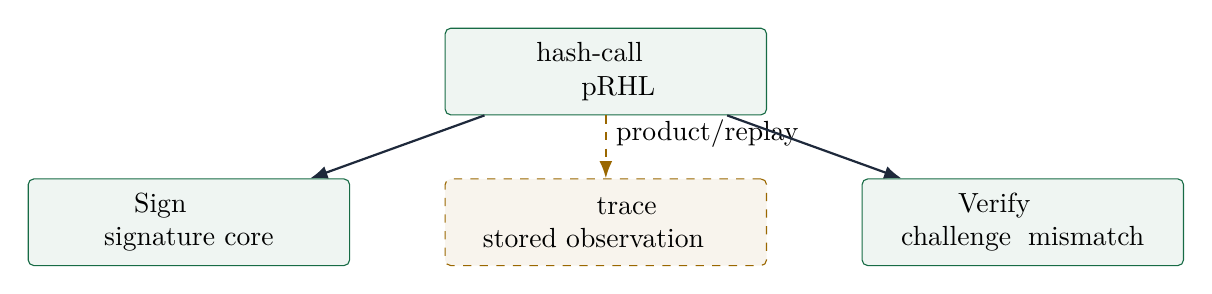
\begin{tikzpicture}[node distance=8mm]
  \node[provennode] (returns) {hash-call 시점의\\두 반환값 pRHL 관계};
  \node[partialnode, below=of returns] (stored) {완료된 두 trace의\\stored observation 관계};
  \node[provennode, left=12mm of stored] (signcont) {Sign의 잔여 실행\\signature core};
  \node[provennode, right=12mm of stored] (verifycont) {Verify의 잔여 실행\\challenge와 mismatch};
  \draw[openarrow] (returns) -- node[right,align=left]{product/replay\\운송 부재} (stored);
  \draw[flowarrow] (returns) -- (signcont);
  \draw[flowarrow] (returns) -- (verifycont);
\end{tikzpicture}
\end{center}

hash-call의 pRHL goal에는 \(res\{1\},res\{2\}\)가 있지만 전체 trace가 끝난
unary post-state에는 이 지역 반환변수가 사라진다. 반대로 hash-call 지점에서
pRHL 정리(theorem)를 적용하면 Sign과 Verify의 서로 다른 잔여 continuation을 처리해야
한다. Sign 쪽 continuation을 일방적으로 버리려면 아직 없는 losslessness 또는
적절한 product rule이 필요하다.

\begin{openobligation}[\claimid{OBL-MU-PRODUCT-REPLAY}]
반환값 수준의 region-local pRHL 정리(theorem)를 이미 완료된 sequential trace의 stored
observation 관계(relation)로 운반하는 sound rule 또는 증명 구조가 필요하다.
\end{openobligation}

이 의무는 Week~7에 \statusdeferred / explicit paper boundary로 동결되었다
\cite{product-replay}. 다음 접근은 의도적으로 거부되었다.

\begin{itemize}
  \item observation equality를 전제로 가정하여 결론을 재진술하기;
  \item SHAKE locality axiom을 새로 추가하기;
  \item 또 다른 caller/observation wrapper로 theorem surface를 계속 넓히기;
  \item termination 근거 없이 Sign continuation을 버리기.
\end{itemize}

따라서 \(\delta_{\mu,\mathrm{raw\_api\_accept}}=0\)은 현재 주장하지 않는다.
이것은 byte-locality 정리(theorem)가 부족해서가 아니라 프로그램 논리의 운송 화살표가
없어서 생긴 의미론 간극이다.

\subsection{accepted-path와 legitimate-signature correctness는 다른 방향이다}

실제 Verify에 대해 증명된 방향은
\[
  \operatorname{Accept}\Longrightarrow\operatorname{TailReached}
  \Longrightarrow\operatorname{HashInputsBound}
\]
이다. 이는 이미 accept한 실행을 분석하는 security-facing lane이다.

기능정확성에 필요한 방향은
\[
  \sigma\leftarrow\operatorname{Sign}(sk,M)
  \Longrightarrow
  \operatorname{Verify}(vk,M,\sigma)=\operatorname{Accept}
\]
이다. 이를 위해서는 Sign이 만든 서명이 unpack/norm/hint/challenge gate를 모두
통과한다는 사실이 필요하다. 첫 방향의 정리(theorem)를 둘째 방향으로 뒤집을 수 없다.

\begin{openobligation}[\claimid{OBL-SIGN-OUTPUT-TAIL-REACH}]
실제 Sign output이 실제 Verify의 early-reject tree를 통과해 tail에 도달함을
증명해야 한다. 현재 signature prefix inverse와 성공 조건부 full-HBZ wrapper는
닫혔고, fixed all-zero HBZ의 반환 실행에서는 failure도 배제되었다. 그러나 이
고정 입력은 실제 Sign output 전체의 canonicality를 대신하지 않는다. \(h\)
suffix, metadata/padding, norm, hint, arithmetic correctness가 남아 있다.
\end{openobligation}

\claimid{OBL-SIGN-VERIFY-CORRECTNESS}는 이 의무와 나머지 산술·challenge
정확성에 막혀 \statusblocked 다.

\subsection{full signature codec에서 남은 표현론}

prefix의 단면--수축(section--retraction)을 full codec으로 확장하려면 적어도
다음 사각형(square)이 필요하다. Week~14에는 이 중 HBZ 간선 하나가 닫혔고,
Week~15에는 그 간선의 fixed all-zero 반환 실행에서 failure가 배제되었다.

\begin{itemize}
  \item 두 size-delta metadata byte가 pack/unpack에서 같은 크기를 나타냄;
  \item HBZ rANS actual full wrapper가 성공 조건 아래 역함수(inverse function)임
        (\statusproved, Week~14);
  \item canonical all-zero HBZ의 fixed-input Hoare success
        (\statusproved, Week~15; termination은 미증명);
  \item 두 번째 \(h\) suffix codec의 encode/decode
        (\statusdeferred, Week~16 MINCORE 전환);
  \item trailing zero padding의 정준성(canonicality)과 parser의 zero gate;
  \item packer/unpacker가 목표 밖 배열 tail을 보존함;
  \item 실제 Sign이 canonical 입력과 성공 buffer bound를 산출함.
\end{itemize}

따라서
\claimid{OBL-SIG-PREFIX-CODEC}은 제한된 의미에서 \statusproved 지만,
\claimid{OBL-SIG-FULL-CODEC-MODE2}는 \statusblocked 다. prefix inverse와 full
inverse를 같은 명제(proposition)로 부르면 안 된다.

\subsection{대수(algebra)·수치(numerics)·확률(probability) 층(layer)에 남은 의무}

frozen paper의 MINCORE 전선은 KeyGen \identifier{STOP-KG-NTT}, Sign
\identifier{STOP-SIGN-CHAL-MODE2}, Verify \FrozenPaperGate 로 정리되었다.
post-freeze에는 \identifier{rq_mul_coeff_foldr_to_bigi}, full-NTT spectral action,
native \(R_q\) 행곱과 HAETAE 표현 운송이 닫혔지만, actual ExpandVecA와 기존
security-side synthetic object의 의미론 불일치가 \CurrentGate 를 만든다.
이와 별개로 actual Verify의 2-by-4 NTT/CRT/freeze 절차 의미론도 frozen
의무로 남는다. 전체 구현 refinement에는 다음 독립적인 의무들이 남는다.

\begin{description}[leftmargin=39mm,style=nextline]
  \item[public-key algebra/NTT]
    \(R_q\)-모듈(module) 계산, NTT 표현, public-key 관계가 실제 구현과 일치함.
  \item[sampler distribution]
    uniform/small/hyperball sampler와 실제 random tape의 출력분포(output
    distribution)가 논문 분포(distribution)와 일치하거나 명시적 거리
    상계(distance bound)를 가짐.
  \item[rejection과 종료]
    KeyGen/Sign retry가 종료하고, 수락 분포(accepted distribution)와 retry loss가
    계산됨.
  \item[highbits/LSB]
    실제 coefficient decomposition, rounding, packing이 논문의
    정수 분해(integer decomposition)와
    일치하며 challenge 양쪽 입력이 같음.
  \item[FIPS202 transcript]
    모든 domain separator, 길이, absorb 순서, squeeze 길이가 고정 명세와
    byte-for-byte 일치함.
  \item[FFT tie policy]
    fixed-point FFT와 경계 동률 처리까지 analytic predicate와 연결됨.
  \item[two-transcript extraction]
    실제 byte-level challenge와 accepted signature instance를 paper/ROM reduction의
    두 transcript 추출에 연결함.
\end{description}

\subsection{Week 16 frozen KeyGen의 KG--NTT--MUL 종료 경계}

actual \identifier{_kp_m23_matrix}와 \identifier{_keypair_finalize_m23}의
투명한 two-call harness는 pre-finalization \(bp\) snapshot, finalizer semantics,
KG-2-like low/high 분해, adjusted \(s_2\), snapshot-only mod-\(2q\) 영 합동식을
같은 사후조건에 둔다
\cite{week16-mincore-plan,week16-kg-report,week16-kg-ntt-mul-report}. 이는
\claimid{OBL-MINCORE-KEYGEN}의 실제 coefficient 경계에서 의미 있는
\statuspartial 진전이다.

matrix helper의 결과는 \identifier{KeygenM23ArithmeticSpec.output_row}로
표현된다. 새 \theoremname{output_row_from_mode2_ntt_words}는 이것을 actual full
NTT, pointwise row product, inverse NTT와 Montgomery 표현으로 정확히 rewrite하며,
\theoremname{actual_m23_matrix_snapshot_rows_explicit}는 투명한 harness의 두 active
row에 그 표현을 적용한다.
frozen paper 시점에는 그 spectral 표현이 native \(R_q\) negacyclic 곱과 같다는
compiled 정리와, \identifier{Rq.poly}를 보안 모형의
\(A_{\mathrm{gen}}s_{\mathrm{gen}}\) 표현으로 옮기는 어댑터가 없었다.
KG-NTT-MUL 감사는 누락 leaf를 odd-root orthogonality/full-NTT convolution과
이 어댑터로 특정하고 \identifier{STOP-KG-NTT}로 종료했다. frozen 판정에서
다음 승격은 금지된다.

\begin{itemize}
  \item snapshot의 \(\mathit{pre\_bp}\)를 근거 없이
        \(A_{\mathrm{gen}}s_{\mathrm{gen}}\)으로 이름 바꾸기;
  \item KG-2-like coefficient 분해에서 faithful KG-1 또는 KG-3를 결론내기;
  \item adjusted \(s_2\) 한 성분에서 complete KG-4 vector를 결론내기;
  \item snapshot 합동식을 논문식 \(A s=qj\pmod{2q}\)로 승격하기;
  \item 이 two-call harness에서 sampler, retry, packing, public API 또는 KeyGen
        종료성을 추론하기.
\end{itemize}

\subsection{post-freeze KG 진전과 새로운 의미론 경계}

frozen 뒤의 shared NTT theory는 pure coefficient normalization, full-NTT
spectral action과 임의 열 수 행곱을 증명했다. Mode~2에서는 KeyGen 3열 및 Verify
4열의 순수 specialization이 모두 컴파일된다. KeyGen 쪽은 native \(R_q\) 행곱에서
\identifier{HAETAE_Algebra.poly_dot}까지 운송되었다
\cite{post-freeze-kg-rq-haetae-report}. 단, Verify 4열 정리는 actual helper
loop를 열지 않으므로 \FrozenPaperGate 를 해제하지 않는다.

다음 감사는 actual \identifier{avec}의 SHAKE128 framing, nonce 515/516,
little-endian candidate와 \(<64513\) rejection을 paper \(a\)에 연결하고 paper
\(qj=q(1,0)^T\)를 snapshot zero equation에 독립적으로 더했다. 그러나 다음 세
대상은 서로 같지 않다.

\begin{center}
actual SHAKE128/rejection \(a\)
\(\neq\) synthetic security generator,
\qquad paper \(qj\)는 별도 correction.
\end{center}

compiled counterexample는 security-named row~0 coefficient~0이 401이고 paper
\(qj[0,0]=64513\)임을 보인다. all-zero seed trace의 actual 값도 44985다.
따라서 \CurrentGate 의 수리는 synthetic
\identifier{public_rounding_vector_seed}를 actual expansion 의미론으로 교체 또는
정제하고 coefficientwise actual-array representation을 증명하는 일이다
\cite{post-freeze-kg-actual-avec-qj-report}. 이 경계를 넘기 전에는 다음 승격도
금지된다.

\begin{itemize}
  \item synthetic object를 actual \identifier{avec} 또는 paper \(qj\)로 재명명;
  \item 별도 \(qj\) correction을 modulo-\(q\) HAETAE vector 안에서 보존된다고 가정;
  \item 새 actual-carrier 전용 coefficient-product를 기존 security
        matrix/secret만으로 정의한 일반 ring \identifier{matrix_vec_mul} 정리 없이
        security-level width-6 mod-\(2q\) 식으로 재명명;
  \item deterministic partial correctness에서 sampler distribution, uniformity,
        losslessness 또는 termination을 추론.
\end{itemize}

\sourcepath{KgFaithfulAugmentedModel.ec}는 이 포장을 위한 actual width-6 carrier와
generated-product transport를 정의하고 standalone fresh compile을 통과한다.
\theoremname{actual_faithful_augmented_productE}는 전용 structured
coefficient-product를 head, generated HAETAE \identifier{poly_dot}, adjusted
error의 합으로 전개한다.
\theoremname{checked_mode2_parent_m23_finalize_faithful_augmented_paper_as_qj}가
actual checked parent에 대해 이 product와 faithful \(qj\)의 합동식을
coefficientwise 증명한다. product는 actual matrix/secret만을 입력으로 받으며,
중간 2-by-3 block은 명시된 열에서 복원된 \identifier{poly_dot}이다.
따라서 이 작업의 판정은 \FaithfulAugmentedVerdict 다. 그러나 이 전용
mod-\(2q\) evaluator는 기존 mod-\(q\) security \identifier{matrix_vec_mul}이 아니고,
security-side ExpandVecA equivalence도 아니다. 따라서 \CurrentGate 가 사라지지는
않는다.

\sourcepath{ImplementationSecurityGoals.ec}는 이 항목들을
\identifier{obl_*} operation으로 열거한다. 이 파일이 컴파일된다는 것은
목표의 이름과 합성 인터페이스가 well-formed하다는 뜻이지 각 boolean이
참임을 증명했다는 뜻이 아니다.

\subsection{최상위 기능정확성은 아직 명세다}

\sourcepath{TopLevelGoals.ec}는
\begin{align*}
  \mathsf{FC}_{\mathrm{KG}}
    &:\quad \mathsf{JKeyGen}_2=\mathsf{PaperKeyGen}_2,\\
  \mathsf{FC}_{\mathrm{Sign}}
    &:\quad \forall sk,M,
      \mathsf{JSign}_2(sk,M)=\mathsf{PaperSign}_2(sk,M),\\
  \mathsf{FC}_{\mathrm{Verify}}
    &:\quad \forall vk,M,\sigma,
      \mathsf{JVerify}_2(vk,M,\sigma)
      =\mathsf{PaperVerify}_2(vk,M,\sigma)
\end{align*}
를 boolean specification으로 둔다. 여기서 Sign/KeyGen의 등식(equality)은
확률분포(probability distribution)의 등식(equality in distribution)을 포함한다.
현재의 prefix, memory, transcript, codec 정리(theorem)는 이 목표에
필요한 결정론적 하위 사각형이지만 전체 등식 자체는 아니다.

\subsection{보안 합성식은 아직 조건부 인터페이스다}

구현과 논문 스킴 사이의 목표는
\[
  \Adv^{\mathrm{euf\mbox{-}cma}}_{\mathrm{Jasmin}}
  \le
  \Adv^{\mathrm{euf\mbox{-}cma}}_{\mathrm{paper}}
  +\delta_{\mathrm{KeyGen}}
  +q_{\mathrm{Sign}}\delta_{\mathrm{Sign}}
  +\delta_{\mathrm{Verify}}
  +\delta_{\mathrm{Encoding}}
\]
의 모양이다. 현재 파일은 손실 변수(loss variable)를 선언하고
부등식(inequality)의 interface를 정의하지만,
각 \(\delta\)를 모두 닫아 최종 정리(theorem)로 합성하지 않았다.

논문 수준 reduction interface는 다시 MLWE, BST-MSIS, ROM 및 rejection/fork
오차로 내려간다. \sourcepath{SecurityAssumptions.ec}는 최종적으로 남길 수 있는
암호학적 인터페이스를 MLWE, BST-MSIS, ROM 세 종류로 제한한다. 하지만 구체적
게임 instance와 매개변수화된 reduction이 구현의 정확한 byte-level scheme에
연결되었다는 뜻은 아니다.

\begin{caution}[선언 종류의 구분]
연산(operation), 가정(assumption), 정리(theorem)는 서로 다르다.
\identifier{op obl_sampler_distribution : bool.}처럼 본문 없이 선언된 operation은
목표를 표현하는 추상 기호(abstract symbol)다. 그것을 참이라고 가정하는 axiom과 동일하지
않고, 그것을 참이라고 증명한 theorem도 아니다. 프로젝트의 검증 스크립트는
authored axiom과 proof hole을 별도로 금지·검색한다.
\end{caution}

\subsection{신뢰 경계와 범위 밖 항목}

현재 증거 사슬은 다음을 신뢰하거나 고정한다.

\begin{itemize}
  \item SHA-256가 기록된 46쪽 HAETAE 명세 PDF \cite{haetae-spec};
  \item pinned \sourcepath{haetae-ref-jasmin/} 구현과 focused extraction
        \cite{pinned-jasmin};
  \item EasyCrypt kernel, Jasmin model, 호출된 SMT prover와 build toolchain;
  \item source hash와 generated extraction/certificate manifest.
\end{itemize}

다음은 이 sprint의 결론에 포함되지 않는다.

\begin{itemize}
  \item mode~2 이외의 parameter set;
  \item 물리적 side channel, fault, RNG 품질;
  \item memory safety나 constant-time이 EUF-CMA에서 자동으로 따라온다는 주장;
  \item 실제 하드웨어/컴파일러 전체의 end-to-end correctness;
  \item full KeyGen, Sign, Verify 또는 구현 EUF-CMA가 완료되었다는 주장.
\end{itemize}

\subsection{현재 주장 행렬}

\begin{longtable}{@{}L{47mm} L{27mm} L{70mm}@{}}
\toprule
주장 & 상태 & 정확한 경계 \\
\midrule
\endfirsthead
\toprule
주장 & 상태 & 정확한 경계 \\
\midrule
\endhead
packed SK의 VK prefix & \statusproved &
실제 generated packer/Internal KeyGen의 반환 시 첫 992바이트 \\
raw \(\mu\) generated seam & \statusproved &
raw branch, 관련 key/pre/message region에서 64-to-32 prefix \\
position-64 challenge suffix & \statusproved &
동일 초기 state/position에서 32-byte absorb \\
actual API key copy/address/frame & \statusproved &
각 명명된 valid/canonical/disjoint 계약 아래 \\
accepted Verify tail/input binding & \statusproved &
accept \(\Rightarrow\) tail/hash inputs 방향 \\
stored observed \(\mu\) equality & \statuspartial &
product/replay transport 부재 \\
signature prefix inverse & \statusproved &
canonical challenge/low, 앞 1056바이트 \\
HBZ leaf inverse & \statusproved &
앞 1024 coefficient, rANS 제외 \\
actual rANS table와 pure step & \statusproved &
concrete 13-symbol table, 명시된 state range \\
pure normalization byte trace & \statusproved &
canonical symbol list, actual loop 아님 \\
actual array/list·word-step bridge & \statusproved &
1024-symbol suffix 점화식(recurrence), literal table word 등식(equality) \\
actual final serialization leaf & \statusproved &
네 번의 실제 store와 누적 trace의 little-endian 직렬화(serialization) 합성 \\
actual encoder success size & \statusproved &
반환한다면 실패이거나 \(0\le off\le1020\), \(4\le1024-off\le1024\) \\
actual inner normalization & \statusproved &
byte segment·frame·no-underflow와 정확한 순수 \(0..2\) exit \\
actual encoder trace refinement & \statusproved &
성공 조건부 부분정확성(success-conditioned partial correctness)의 전체 suffix 등식(equality) \\
actual decoder trace refinement & \statusproved &
exact-trace 부분정확성(partial correctness), 1024-symbol 등식(equality), 정확한 byte 소비와 tail frame \\
actual rANS harness control & \statusproved &
실제 호출 순서와 성공/실패 분기만 완료 \\
actual rANS core inverse & \statusproved &
actual encoder/copy/decoder의 성공 조건부 부분정확성(success-conditioned partial correctness) \\
actual encoder success witness & \statusproved &
fixed all-zero/all-6 반환 실행의 failure exclusion; termination/losslessness 없음 \\
production full-HBZ wrapper inverse & \statusproved &
prepare/apply, rANS core와 production lift의 성공 조건부 합성 완료 \\
actual KeyGen matrix/finalize snapshot & \statuspartial &
KG-2-like 분해와 snapshot mod-\(2q\) identity는 증명;
frozen paper에서는 마지막 NTT-word rewrite 뒤 \identifier{STOP-KG-NTT} \\
post-freeze NTT/Rq/HAETAE 행곱 & \statusproved &
순수 spectral action, native \(R_q\) 3열/4열 행곱과 KeyGen 3열 HAETAE 표현 운송;
actual Verify procedure는 제외 \\
post-freeze actual \identifier{avec}/paper \(a,qj\) & \statuspartial &
결정론적 expansion과 별도 \(qj\) snapshot 합성은 증명;
synthetic security 의미론 불일치에서 \CurrentGate \\
faithful augmented coefficient-product 합성 & \statusproved &
standalone actual-carrier structured product \(\equiv qj\); frozen 82-target 밖이며
generic security-model \identifier{matrix_vec_mul}/ExpandVecA equivalence는 제외 \\
actual Sign accepted core & \statuspartial &
실제 세 helper의 호출·accept branch control만;
\identifier{STOP-SIGN-CHAL-MODE2} \\
actual Verify core sequence & \statuspartial &
실제 다섯 helper 순서, V-1/V-2/V-5/V-6 word projection, norm/tail local 결과;
frozen \FrozenPaperGate \\
\(h\) suffix codec & \statusdeferred &
Week~16 MINCORE KeyGen 범위 전환; inverse 미시도 \\
full signature codec & \statusblocked &
HBZ wrapper 뒤에도 \(h\), metadata, padding과 residual frame 잔여 \\
Sign output tail reach & \statuspartial &
prefix와 success-conditioned HBZ wrapper만 닫힘; \(h\), metadata/padding,
norm/hint/arithmetic 잔여 \\
FC-KeyGen/Sign/Verify & \statusspecified / \statuspartial &
KeyGen snapshot 포함 하위 결정론적 seam만 일부 증명 \\
구현 EUF-CMA & \statusspecified &
loss와 paper reduction 연결 미완 \\
\bottomrule
\end{longtable}

\section{의존성에 따른 다음 작업과 참여 지점}
\label{sec:roadmap}

\subsection{현재 단일 우선순위: security ExpandVecA 의미론 수리}

최신 post-freeze gate는 \CurrentGate 다. 첫 의무는
\begin{quote}
\CurrentPriority
\end{quote}
이다. post-freeze NTT/Rq/HAETAE 운송과 actual \identifier{avec}의 paper \(a\)
해석은 컴파일되었다. 그러나 기존 security-side object는 actual SHAKE128/rejection
expansion도 paper \(qj\)도 아닌 synthetic generator다. 이 불일치를 고치지 않은
채 전체 KeyGen 식을 합성하면 concrete coefficient 44985와 401을 같다고 놓게 된다.
한편 frozen paper의 \FrozenPaperGate 는 별도 상태다. 순수 2-by-4 행곱
specialization이 post-freeze에 생겼어도 actual Verify helper loop와 CRT/freeze
절차 정리는 여전히 열려 있다.

\begin{figure}[ht]
\centering
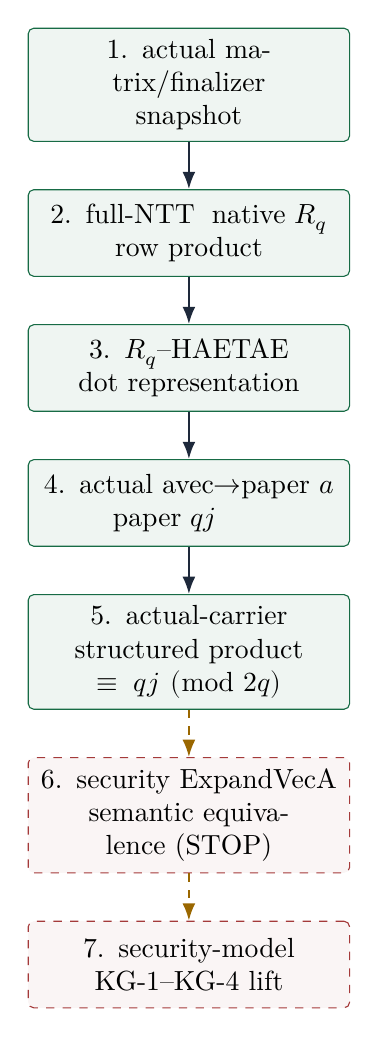
\begin{tikzpicture}[node distance=6mm]
  \node[provennode] (snapshot) {1. actual matrix/finalizer\\snapshot};
  \node[provennode, below=of snapshot] (ntt) {2. full-NTT와 native \(R_q\)\\row product};
  \node[provennode, below=of ntt] (repr) {3. \(R_q\)--HAETAE\\dot representation};
  \node[provennode, below=of repr] (avec) {4. actual \identifier{avec}\(\to\)paper \(a\)\\paper \(qj\) 별도 합성};
  \node[provennode, below=of avec] (faithful) {5. actual-carrier structured product\\\(\equiv qj\pmod{2q}\)};
  \node[blockednode, below=of faithful] (security) {6. security ExpandVecA\\semantic equivalence (STOP)};
  \node[blockednode, below=of security] (paper) {7. security-model\\KG-1--KG-4 lift};
  \draw[flowarrow] (snapshot) -- (ntt);
  \draw[flowarrow] (ntt) -- (repr);
  \draw[flowarrow] (repr) -- (avec);
  \draw[flowarrow] (avec) -- (faithful);
  \draw[openarrow] (faithful) -- (security);
  \draw[openarrow] (security) -- (paper);
\end{tikzpicture}
\caption{post-freeze KeyGen의 현재 절단면. actual-carrier 전용 coefficient-product까지
닫혔지만, generic security ExpandVecA/\identifier{matrix_vec_mul} 의미론에서 중단했다.}
\label{fig:next-order}
\end{figure}

codec 선에서는 Week~15에 fixed all-6 반환 실행의 failure exclusion까지 닫혔다.
그러나 fixed-input termination/losslessness는 열려 있고, \(h\) suffix codec은
이번 one-week MINCORE 범위 전환으로 \statusdeferred 되었다. 이 두 사실은 현재
KeyGen blocker와 독립적이다.

\subsection{1단계 완료: encoder}

\claimid{OBL-RANS-ENCODE-REFINEMENT}는 실제
\identifier{_rans_encode}를 여는
\theoremname{actual_rans_encode_trace_closure}와 그 확장된 따름정리(corollary)
\theoremname{actual_rans_encode_trace_refinement}로 닫혔다. 성공 분기(success
branch)의 사후조건(postcondition)은 다음을 동시에 준다.

\begin{itemize}
  \item actual output suffix가 canonical symbol list의
        \identifier{trace_bytes}와 점별로 같음;
  \item 바깥 반복(outer iteration)마다 actual word state가 suffix의 순수
        \identifier{encode_trace} state와 같음;
  \item actual \(off\)와 trace byte 길이가
        \(off+|\operatorname{TraceBytes}|=1024\)를 만족함;
  \item 이미 증명된 final 4-byte state 직렬화(serialization)를 normalization
        suffix 앞에 합성하여 segment 순서를 확정함;
  \item 쓰지 않은 접두부(unwritten prefix)의 frame을 유지함;
  \item 실패 branch를 숨기지 않음.
\end{itemize}

Week~10의 array/list suffix 점화식(recurrence), actual reciprocal word step,
내부 byte/frame/no-underflow, final serialization leaf와 성공 offset/size 범위는
Week~11의 tail-aware 바깥/안쪽 불변식(outer/inner invariant), generated table
load--protect--word-update 보조정리(lemma), final-store 합성(composition)에
연결되었다. 따라서 임의의 valid trace나 새 증인 버퍼(witness buffer)가 아니라
실제 반환 버퍼의 suffix가 정준 trace 바이트(canonical trace bytes)와 일치한다.

다만 이는 Hoare 부분정당성(Hoare partial correctness)이다. 실제 실행이 성공
분기(success branch)에 도달한다는 성공 증인(success witness)과 종료성(termination)은
이 Week~11 정리 하나에서 따라오지 않는다. Week~15는 fixed all-6 반환 실행의
failure를 별도 정리로 배제했지만 종료성은 여전히 남는다.

\subsection{2단계 완료: decoder}

\claimid{OBL-RANS-DECODE-REFINEMENT}는 실제
\identifier{_rans_decode}를 여는
\theoremname{actual_rans_decode_trace_refinement}로 닫혔다. exact-trace 입력
관계(input relation) 아래 다음이 귀납법(induction)으로 증명되었다.

\begin{itemize}
  \item iteration \(i\)에서 decoded prefix가 원래 symbol prefix와 같음;
  \item state/cursor가 pure \(x_i,c_i\)와 같음;
  \item actual table lookup이 구간 분할(interval partition)의 유일한 \(s_i\)를 선택함;
  \item nested normalization loop가 \(\beta_i\)를 정확한 순서로 소비함;
  \item 내부 loop 종료에서 \(state=2^{23}\)을 유도하고, 반환값에서
        \(off=size\), \(bad=0\)을 결론냄;
  \item decoded tail frame.
\end{itemize}

encoder와 decoder를 직접 lockstep으로 묶는 방법은 reverse/forward 방향과
중간 buffer copy 때문에 proof surface가 커진다. 이미 구성된 순수 trace를
공통 매개체로 삼아 두 refinement를 독립적으로 검증했다. 단, 이 decoder
정리(theorem)는 입력 trace를 전제로 받는 Hoare 부분정당성(Hoare partial
correctness)이며 종료성(termination)을 주지 않는다.

\subsection{3단계 완료: actual harness inverse}

\claimid{OBL-RANS-CORE-INVERSE}는
\sourcepath{Mode2RansCoreActualInverse.ec}의
\theoremname{actual_rans_encode_copy_decode_inverse}로 닫혔다. 이 정리(theorem)는
\sourcepath{Mode2RansActualInverse.ec}에 정의된 actual harness를 직접 대상으로
삼아 다음 의미론적 결론을 낸다. 두 파일명은 각각 ``harness 정의/control''과
``Week~13 semantic inverse''를 가리키며, 후자는 전자의 control-only 정리(theorem)를
의미론적 결과로 잘못 읽지 않도록 별도 증명된 것이다.

\begin{itemize}
  \item encoder 실패 분기(failure branch)를 숨기지 않고 decoder를 실행하지 않음;
  \item encoder 성공 suffix의 \identifier{segment_matches}를 actual copy의
        \identifier{slice_eq}에 합성함;
  \item copy된 buffer에서 decoder의 pointwise exact-read 전제를 산출함;
  \item actual decoder 반환에서 \(bad=0\), exact consumption, 1024-symbol
        등식(equality), tail frame을 얻음;
  \item 임의의 trace, 새 증인 버퍼(witness buffer), encoder 성공을 외부 전제로
        넣지 않음.
\end{itemize}

이 정리(theorem)는 성공 조건부 부분정확성(success-conditioned partial
correctness)이다. canonical all-zero array는 전제의 비공허성(non-vacuity)을
보이지만, encoder 성공의 존재나 전체 실행의 종료성(termination)을 자동으로
주지 않는다. Week~13 당시 성공 도달성은
\claimid{OBL-RANS-ACTUAL-SUCCESS-WITNESS}의 별도 의무였고, Week~15는 그중
fixed all-6 Hoare 사후조건만 닫았다.

\subsection{4단계 완료: production full-HBZ wrapper}

\claimid{OBL-SIG-HBZ-ENCODE-DECODE}는
\theoremname{signature_pack_unpack_hbz_full_actual_exact}와
\theoremname{signature_pack_unpack_hbz_full_inverse_mode2}로 닫혔다. actual
\identifier{_encode_hb_z1_full}과 \identifier{_decode_hb_z1_full}을 직접 여는
사슬은 다음을 결론낸다.

\begin{itemize}
  \item canonical HBZ coefficient를 actual prepare가 정준 기호열(canonical
        symbol stream)로 옮김;
  \item actual rANS core 정리(theorem)의 실패/성공 분기를 그대로 보존함;
  \item 성공 시 actual apply가 복원된 symbol을 원래 coefficient로 되돌림;
  \item wrapper-level size, state, 입력/출력 tail frame을 연결함;
  \item actual success witness나 decoder 결과를 외부 전제로 다시 요구하지 않음.
\end{itemize}

이 단계는 성공 조건부 부분정확성(success-conditioned partial correctness)으로
\statusproved 다 \cite{week14-report,hbz-full-wrapper-composition}. 실제 성공
가지의 일반 도달가능성(reachability)과 종료성(termination)은 별도
정리(theorem)다. Week~15는 fixed all-zero 입력의 반환 실행에 한해 failure를
배제한다.

\subsection{5단계 완료: fixed all-6 success 사후조건}

Week~15의 \theoremname{actual_rans_encode_all_six_success}는 actual failure가
trace length \(>1020\)을 요구한다는 정리와 all-6 trace의 \(\le1020\) budget을
모순시켜 반환하는 fixed-input 실행의 \(bad=0\)을 얻는다. focused/production
lift는 \(4\le size\le1024\), exact trace/frame과 zero coefficient round trip을
동시에 보인다 \cite{week15-report,rans-actual-success-witness}.

이 단계의 완료 판정은 fixed-input Hoare 부분정확성이다. termination,
losslessness, non-vacuous execution 또는 \identifier{phoare}로 승격하지 않는다.
원래 뒤따를 예정이던 \(h\) suffix, metadata/padding, full signature inverse와
Sign output tail reach는 Week~16 MINCORE 전환으로 각각 deferred 또는 blocked
상태를 유지한다.

\subsection{6단계 frozen 종료: KG--NTT--MUL 감사}

\theoremname{output_row_from_mode2_ntt_words}와
\theoremname{actual_m23_matrix_snapshot_rows_explicit}는
\identifier{KeygenM23ArithmeticSpec.output_row}를 actual full-invNTT/pointwise
word 표현으로 rewrite하고 두 active row에 적용하는 마지막 sound edge를 닫았다
\cite{week16-kg-ntt-mul-report}. frozen paper 시점에는 다음 두 화살표가 없었다.
\[
  \operatorname{array256\_mont}
    (\operatorname{full\_invntt}(\widehat a\odot\operatorname{full\_ntt}(p)))
  \;\not\Longrightarrow\;
  (\operatorname{full\_invntt}\widehat a)\star_{R_q}p,
\]
그리고 native \identifier{Rq.poly} 곱을 보안 모형의 integer-list
\identifier{poly_mul}/\identifier{matrix_vec_mul}로 옮기는 어댑터도 없다. 첫
화살표에는 odd-root orthogonality와 full-NTT convolution이 필요했다. 시간 제한
감사는 이를 새 전제로 가정하지 않고 \identifier{STOP-KG-NTT}로 종료했다.
post-freeze에 이 순수 대수와 \(R_q\)--HAETAE 표현 간극은 닫혔지만, 이 역사적
frozen 판정 자체는 변경하지 않는다.

\subsection{7단계 동결: accepted Sign core}

다음 세 actual helper의 순차 실행은 투명한 harness에서 합성되어 control
정리까지 컴파일됐다.
\begin{center}
\identifier{_sf_round_challenge_mode2}\quad
\identifier{_sf_z_check}\quad
\identifier{_sf_hint_mode2}
\end{center}
컴파일된 control theorem은
\sourcepath{Mode2SignAcceptedCore.ec}의
\begin{center}
\theoremname{actual_sign_accepted_core_branch_control_mode2}
\end{center}
이다. 그러나 headline S-1--S-7 정리는
\identifier{sf_challenge_mode2_highbits_lsb_sampleinball_correct} 부재로
\identifier{STOP-SIGN-CHAL-MODE2}에서 동결되었다.
반환하고 accept한 실행에 대해 commitment/challenge, response
\(z=y+(-1)^bcs\), 두 exact integer norm predicate와 coefficientwise hint 식을
도출해야 한다 \cite{week16-mincore-plan,claim-ledger}.

headline 정리는 아직 컴파일된 증명으로 세어서는 안 된다.
사전조건이 \identifier{reject=0}이나 최종 식을 가정해서도 안 된다. sampler
분포, signing-loop 종료성, packing과 전체 1474-byte signature는 이 단계의 범위
밖이다.

\subsection{8단계 frozen 종료: actual Verify helper chain}

\sourcepath{Mode2VerifyCoreSequence.ec}의
\theoremname{actual_verify_core_sequence_branch_control_mode2}와
\theoremname{actual_verify_core_sequence_input_snapshots_mode2}는 actual
Verify의 다섯 helper 호출 순서와 입력 snapshot을 고정한다.
\sourcepath{Mode2VerifyPrepareNorm.ec},
\sourcepath{Mode2VerifyRecover.ec},
\sourcepath{Mode2VerifyTailChallenge.ec}는 각각
\theoremname{verify_prepare_z1_wprime_mode2_word_exact},
\theoremname{actual_sign_verify_recover_w_z2_mode2_word_semantics},
\theoremname{verify_tail_exact_trace_mode2}와
\theoremname{poly_mismatch_mode2_word_exact}를 제공한다
\cite{week16-verify-report}. 따라서 V-1/V-2/V-5/V-6 projection, W64 norm gate,
tail trace/mismatch expression은 helper-local 범위에서 닫혔다.

그러나 actual 2-by-4
\identifier{_polyvec_ntt}/\identifier{_polymat_pointwise_acc}/
\identifier{_polyvec_invntt}의
\identifier{verify_matrix_ntt_acc_mode2_cols4_correct}와 actual from-CRT/freeze의
\identifier{verify_crt_freeze_mode2_word_exact}가 없다. challenge leaf
\identifier{verify_tail_m23_highbits_lsb_sampleinball_correct}도 독립적으로 남는다.
이것이 frozen \FrozenPaperGate 다. post-freeze의 pure
\theoremname{verify_mode2_row_product_from_reprs}는 첫 절차 leaf의 대수적 목표를
주지만 actual loop refinement를 대신하지 않는다.

\subsection{9단계 진행: post-freeze actual avec/qj 감사}

\theoremname{rq_mul_coeff_foldr_to_bigi}, full-NTT spectral action, generic row
product, native \(R_q\) 3항 곱과 HAETAE dot representation은 이제
\statusproved 다. actual sampler 쪽도 nonce 515/516, SHAKE128 framing,
little-endian parsing, \(<64513\) rejection과 unchanged storage를 paper \(a\)로
해석하며 paper \(qj\)를 snapshot equation에 별도로 합성한다
\cite{post-freeze-kg-rq-haetae-report,
post-freeze-kg-actual-avec-qj-report}.

현재 첫 목표는 \claimid{OBL-KG-SECURITY-EXPANDVECA-SEMANTICS}다. security
\identifier{public_rounding_vector_seed}가 actual expansion과 동일한 semantics를
갖도록 specification을 교체·정제하고, coefficientwise actual-array
representation을 증명해야 한다. 이후에도 paper \(qj\) correction을 별도로
보존하는 actual-carrier width-6 coefficient-product packaging은 최신
\sourcepath{KgFaithfulAugmentedModel.ec}에서 닫혔다. 이 파일은 actual
matrix/secret 구체화, generated HAETAE \identifier{poly_dot} 운송과
\theoremname{actual_faithful_augmented_productE}를 거쳐 actual checked parent의
product \(\equiv qj\pmod{2q}\) 식을 standalone fresh-compiled theorem으로
합성한다. 이 product는 actual matrix/secret만을 입력으로 받고 중간
2-by-3 block을 그 열에서 복원하므로 \FaithfulAugmentedVerdict 로 판정한다.
남은 의무는 이 전용 mod-\(2q\) block semantics를 기존 mod-\(q\), width-4
security model로 잘못 동일시하지 않은 채, synthetic security object를 actual
ExpandVecA semantics로 교체·정제하는 별도 대응 정리다.

각 부모를 닫을 때 자식
정리(child theorem)의 전제가 실제 앞 절차의 결론에서 나오는지 확인해야 한다.
external precondition으로 원하는 등식을 다시 요구하면 합성이 아니라 조건부
재진술이다.

\subsection{동결된 product/replay 선은 별도로 다룬다}

codec 선과 독립적으로 \claimid{OBL-MU-PRODUCT-REPLAY}는 explicit paper
boundary로 남아 있다. 재개하려면 wrapper 추가가 아니라 다음 중 하나가 필요하다.

\begin{itemize}
  \item hash 반환값을 ghost observation에 저장하는 시점까지 보존하는 sound
        relational sequencing lemma;
  \item 두 continuation을 함께 처리하는 product program과 그 semantics;
  \item Sign continuation의 losslessness/termination을 먼저 증명한 뒤 사용할 수
        있는 정당한 one-sided elimination;
  \item hash-time snapshot을 trace가 보존하도록 하는 최소 instrumentation 변경과
        그 actual-to-trace exactness 재증명.
\end{itemize}

어느 선택도 단순한 byte lemma가 아니다. program logic 설계와 theorem surface
trade-off를 먼저 검토해야 한다.

\subsection{순수 대수학자가 바로 기여할 수 있는 문제}

\begin{question}[rANS를 제한된 전단사(restricted bijection)로 패키징하기]
집합(set)
\[
  \mathcal X_s=\{x:2^{23}\le x<2^{31}\},\qquad
  \mathcal N_s=\{r:1\le r<x_{\max}(s)\}
\]
와 0/1/2-byte 섬유(fiber)를 사용해 normalization--fast-step을 명시적인
부분 전단사(partial bijection)로 패키징할 수 있는가? 현재 개별 lemma를 actual
loop invariant에서 재사용하기 쉬운 하나의 귀납 정리(induction theorem)로 묶는
것이 목표다.
\end{question}

\begin{question}[표현의 몫(quotient)과 정준 단면(canonical section)]
signature 각 구성요소에 대해 raw word 공간(word space), 바이트 몫(byte quotient),
정준 대표자계(canonical system of representatives), decoder 단면(section)을 한
번에 기술하는 공통 구조를 만들 수 있는가?
새 추상화는 실제 기존 술어를 재사용하고, prefix/HBZ/향후 \(h\) codec의
중복만 제거해야 한다.
\end{question}

\begin{question}[ExpandVecA, \(R_q\), mod-\(2q\) 표현]
닫힌 NTT·\(R_q\)·HAETAE 결과의 정확한 명제(proposition)/전제(premise)를
유지하면서 actual SHAKE128/rejection \identifier{avec}를 faithful security
matrix로 어떻게 표현할 수 있는가? paper \(qj\) correction을 modulo-\(q\)
vector와 혼합하지 않고, 새 actual-carrier structured coefficient-product를
augmented matrix/secret만의 generic ring \identifier{matrix_vec_mul} 및 security
model에 어떻게 연결할 수 있는가? Verify 쪽은
동일한 순수 4열 행곱을 actual NTT/CRT/freeze procedure theorem에 연결하는 별도
가환사각형(commutative square)이 필요하다.
\end{question}

\begin{question}[high/low decomposition의 정수 경계(integer bound)]
논문의 \(r=\alpha\operatorname{HighBits}(r)+\operatorname{LowBits}(r)\)와
실제 고정폭 rounding/sign-extension/packing 사이의
정준 대표자(canonical representative) 조건을 정확히
분리할 수 있는가? 이 작업은 전체 challenge input과 norm/hint correctness의
대수적 중심이다.
\end{question}

\begin{question}[rejection distribution]
partial map으로 모델링된 retry loop를 확률 커널(probability kernel)로 올리고,
수락 분포(accepted distribution)와 termination/loss bound를 논문 sampler에
연결할 수 있는가?
결정론적 Hoare 정리(deterministic Hoare theorem)와
분포 정리(distribution theorem)를 섞지 않는 interface 설계가 필요하다.
\end{question}

\subsection{대수기하학자의 기술이 유용한 곳}

현재 작업이 스킴 이론적(scheme-theoretic) 증명은 아니지만 다음 습관은 직접
유용하다.

\begin{itemize}
  \item 전체 객체(object) 대신 필요한 제한(restriction)만 비교하는
        국소--대역(local-to-global) 사고;
  \item 서로 다른 표현 좌표(chart) 사이의 전이사상(transition map)과
        호환성(compatibility) 도식을 명시하는 습관;
  \item 몫(quotient)과 대표 단면(representative section)을 분리하는 습관;
  \item 섬유(fiber)가 비어 있지 않음을 witness로 확인하고,
        조건부 정리(conditional theorem)의
        non-vacuity를 점검하는 습관;
  \item 큰 목표를 가환사각형(commutative square)과 장애물(obstruction)로
        분해하는 습관.
\end{itemize}

단, 이 습관을 ``현재 코드가 층(sheaf)을 형식화한다''는 주장으로 바꾸면 안 된다.
실제 proof term은 배열, word, 메모리, procedure semantics 위에 있다.

\subsection{새 정리(theorem)를 제출할 때의 판정 체크리스트}

\begin{enumerate}
  \item 정리(theorem)의 actual/generated/pure 경계를 이름과 주석에 명시했는가?
  \item 부모 결론을 전제로 다시 가정하지 않았는가?
  \item termination, partial correctness, losslessness를 구분했는가?
  \item canonicality, address range, no-wrap, separation 전제가 모두 보이는가?
  \item 반환값, global state, ghost observation 중 무엇을 비교하는지 명시했는가?
  \item 사용하지 않는 배열·메모리 구간의 frame이 필요한가?
  \item 전제의 concrete witness 또는 실제 predecessor가 있어 non-vacuous한가?
  \item authored axiom, admit/sorry/abort, debug declaration이 없는가?
  \item manifest에 들어가 fresh \identifier{-no-eco} compile되는가?
  \item claim ledger와 theorem graph의 부모 상태를 과장 없이 갱신했는가?
\end{enumerate}

이 체크리스트를 통과해야 ``수학적으로 그럴듯함''이 ``현재 구현에 대해
검증됨''으로 바뀐다.

\appendix
\section{정리(theorem)와 소스 인덱스}
\label{sec:source-index}

이 부록은 본문의 수학 문장을 실제 저장소 선언으로 되돌아가기 위한 지도다.
줄 번호는 편집 때 바뀌므로 파일 경로와 정리 식별자(theorem identifier)를
기준으로 한다. 최종
판정은 항상 해당 EasyCrypt 선언의 전제와 최신
\sourcepath{CLAIM_LEDGER.md}를 함께 읽어야 한다.

\subsection{상태와 범위 문서}

\begin{longtable}{L{56mm} L{91mm}}
\toprule
경로 & 역할 \\
\midrule
\endfirsthead
\toprule
경로 & 역할 \\
\midrule
\endhead
\sourcepath{PROJECT_SCOPE.md} & mode~2 범위, 고정 명세, trust boundary,
완료로 주장하지 않는 항목 \\
\sourcepath{CLAIM_LEDGER.md} & claim ID별 운영상 source of truth; status,
실제 Jasmin target, EasyCrypt evidence, 남은 전제 \\
\sourcepath{THEOREM_GRAPH.md} & 최상위 보안 목표에서 leaf 정리(theorem)까지의 의존성 DAG \\
\sourcepath{ASSUMPTIONS.md} & 최종 가정, 구현 계약, non-vacuity,
과장 금지 정책 \\
\sourcepath{PRODUCT_REPLAY_DECISION.md} & stored \(\mu\) product/replay gap의
의미론 분석과 동결 결정 \\
\sourcepath{SIGNATURE_CODEC_OBLIGATIONS.md} & mode~2 signature layout와 staged
codec 의무 \\
\sourcepath{RANS_PROOF_DESIGN.md} & rANS 증명 분해와 설계 선택 \\
\sourcepath{RANS_BYTE_STACK_INVARIANT.md} & reverse encoder와 forward decoder를
잇는 \(xs/cuts/bytes\) invariant \\
\sourcepath{WEEK9_REPORT.md} & 순수 byte stack과 actual control 경계의 역사적
Week~9 기준선 \\
\sourcepath{RANS_ENCODER_INVARIANT.md} & actual encoder 바깥 루프 불변식(outer-loop
invariant), Week~10 설계 경계와 Week~11 actual trace closure \\
\sourcepath{WEEK10_REPORT.md} & 역사적 \identifier{CONTINUE-ENCODER} 판정과
50-target 검증 결과 \\
\sourcepath{WEEK11_REPORT.md} & 역사적 \identifier{GO-ENCODER} 판정과
57-target 검증 결과, actual encoder trace closure \\
\sourcepath{RANS_DECODER_INVARIANT.md} & actual decoder의 순수 state/cursor/segment
좌표(coordinates), outer/inner 불변식(invariants), exact-trace 경계 \\
\sourcepath{WEEK12_REPORT.md} & 역사적 \identifier{GO-DECODER} 판정,
65-target 검증 결과와 actual decoder refinement \\
\sourcepath{RANS_CORE_COMPOSITION.md} & encoder segment, actual copy slice,
decoder pointwise read와 configured state 사이의 Week~13 운송 구조 \\
\sourcepath{MODE2_HBZ_CODEC_OBLIGATIONS.md} & HBZ leaf, rANS core, production wrapper
의무의 최신 층별 상태 \\
\sourcepath{WEEK13_REPORT.md} & 현재 \identifier{GO-CORE} 판정,
67-target 검증 결과, actual core inverse와 full-HBZ wrapper 단일 우선순위 \\
\bottomrule
\end{longtable}

\subsection{packed key와 memory bridge}

\footnotesize
\begin{longtable}{L{50mm} L{49mm} L{46mm}}
\toprule
파일 & 주요 선언 & 수학적 역할 \\
\midrule
\endfirsthead
\toprule
파일 & 주요 선언 & 수학적 역할 \\
\midrule
\endhead
\sourcepath{easycrypt/refinement/keygen/PackedKeyPrefix.ec} &
\theoremname{vk_prefix_eq_set_after};
\theoremname{copied_prefix_step};
\theoremname{copied_prefix_complete} &
접두부 동치관계(equivalence relation)의 순수 배열 invariant \\
\sourcepath{easycrypt/refinement/keygen/ExtractedPackedKeyPrefix.ec} &
\theoremname{pack_vec_eta_to_prefix_frame};
\theoremname{pack_vec2_eta_to_prefix_frame};
\theoremname{pack_sk_m23_mode2_vk_prefix} &
actual packer의 접두부와 이후 쓰기 frame \\
같은 파일 &
\theoremname{keypair_full_m23_mode2_return_prefix};
\theoremname{keypair_internal_mode2_return_prefix} &
generated internal KeyGen 반환까지 lift \\
\sourcepath{easycrypt/support/Mode2KeyMemoryBridge.ec} &
\theoremname{keygen_prefix_reaches_mu_memory} &
로컬 배열 prefix를 global-memory load 관계로 번역 \\
\sourcepath{easycrypt/refinement/composition/ApiKeyMemoryBridge.ec} &
\theoremname{keygen_export_vk_mode2_prefix};
\theoremname{keygen_export_sk_mode2_prefix};
\theoremname{sign_import_mode2_sk_prefix};
\theoremname{verify_import_mode2_vk_prefix} &
actual copy helper의 export/import 계약 \\
같은 파일 &
\theoremname{keygen_export_sk_mode2_prefix_frames_vk};
\theoremname{sign_verify_api_importer_same_inputs} &
disjoint frame과 Sign/Verify 입력 연결 \\
\sourcepath{easycrypt/refinement/composition/RawApiAddressBridge.ec} &
\theoremname{canonical_ui64_address_roundtrip};
\theoremname{mode2_vk_region_bridge};
\theoremname{mode2_sk_region_bridge};
\theoremname{mode2_sig_region_bridge} &
canonical integer/\(W64\) 주소 대응 \\
\sourcepath{easycrypt/refinement/composition/RawApiKeygen}\allowbreak
\sourcepath{SequentialExport.ec} &
\theoremname{keypair_raw_api_trace_exports_matching_prefixes};
\theoremname{keypair_raw_api_exports_matching_prefixes} &
실제 raw KeyGen caller의 순차 외부 export \\
\bottomrule
\end{longtable}
\normalsize

\subsection{\texorpdfstring{\(\mu\)}{mu}, challenge, actual API trace}

\footnotesize
\begin{longtable}{L{50mm} L{49mm} L{46mm}}
\toprule
파일 & 주요 선언 & 수학적 역할 \\
\midrule
\endfirsthead
\toprule
파일 & 주요 선언 & 수학적 역할 \\
\midrule
\endhead
\sourcepath{easycrypt/refinement/composition/ExtractedMuHashPrefix.ec} &
\theoremname{sign_sk_verify_vk_absorb_mode2};
\theoremname{sign_verify_final_squeeze_mu32_prefix};
\theoremname{sign_verify_raw_mu_top_wrappers_prefix} &
actual generated helper chain의 key/hash/squeeze 관계 \\
\sourcepath{easycrypt/refinement/composition/ExactMuTopControl.ec} &
\theoremname{raw_prelen_shr63_zero};
\theoremname{raw_prelen_branch_guard} &
실제 Verify 분기의 raw path 선택 \\
같은 파일 &
\theoremname{sf_mu_rawpre_refines_raw_top};
\theoremname{verify_hash_mu_raw_refines_raw_top};
\theoremname{sign_verify_generated_raw_mu_prefix} &
actual generated top 절차의 64-to-32 \(\mu\) relation \\
\sourcepath{easycrypt/refinement/composition/ExactMode2RawMuComposition.ec} &
\theoremname{generated_raw_mu_preconditions_from_keygen_prefix};
\theoremname{generated_raw_mu_to_challenge_suffix_zero_loss} &
KeyGen prefix에서 실제 position-64 challenge absorb까지 \\
\sourcepath{easycrypt/refinement/composition/RegionLocalMuEquivalence.ec} &
\theoremname{region_eq_head};
\theoremname{region_eq_tail};
\theoremname{sign_verify_raw_mu_top_wrappers_prefix_regionwise} &
whole-memory equality를 read-region equality로 약화 \\
\sourcepath{easycrypt/refinement/composition/RegionLocalMuTop.ec} &
\theoremname{sign_verify_generated_raw_mu_prefix_regionwise} &
region-local relation을 actual generated top 절차로 lift \\
\sourcepath{easycrypt/refinement/composition/RawApiSignOutputFrame.ec} &
\theoremname{sign_output_copy_exact_and_frames_reused};
\theoremname{sign_raw_api_frames_reused_regions} &
actual Sign output과 siglen store의 frame \\
\sourcepath{easycrypt/refinement/composition/RawApiVerifyAcceptTrace.ec} &
\theoremname{verify_cryptolab_actual_accept_implies_trace_tail_reached};
\theoremname{verify_cryptolab_actual_accept_binds_hash_inputs} &
accept \(\Rightarrow\) tail과 실제 hash input binding \\
\sourcepath{easycrypt/refinement/composition/RawApiDirectObservedMu.ec} &
\theoremname{raw_sign_then_verify_actual_exact_trace};
\theoremname{sign_then_verify_trace_accept_implies_tail_reached};
\theoremname{sign_then_verify_accept_binds_observed_inputs} &
actual sequential Sign--Verify와 ghost trace의 exactness \\
같은 파일 &
직접 stored \identifier{observed_mu} relation 없음 &
\claimid{OBL-DIRECT-OBSERVED-MU}가 \statuspartial 인 정확한 위치 \\
\bottomrule
\end{longtable}
\normalsize

\subsection{signature prefix와 HBZ leaf}

\footnotesize
\begin{longtable}{L{50mm} L{49mm} L{46mm}}
\toprule
파일 & 주요 선언 & 수학적 역할 \\
\midrule
\endfirsthead
\toprule
파일 & 주요 선언 & 수학적 역할 \\
\midrule
\endhead
\sourcepath{easycrypt/refinement/sign/Mode2SignaturePrefixCodec.ec} &
\theoremname{canonical_challenge};
\theoremname{canonical_signed_low};
\theoremname{prefix_codec_preconditions_satisfiable} &
정준 대표자(canonical representative) 조건과 non-vacuity \\
\sourcepath{easycrypt/refinement/sign/Mode2SignaturePrefixPack.ec} &
\theoremname{pack_sig_prefix_mode2_layout} &
actual pack loop의 challenge/low byte layout \\
\sourcepath{easycrypt/refinement/sign/Mode2SignaturePrefixUnpack.ec} &
\theoremname{unpack_sig_prefix_mode2_layout} &
actual unpack loop의 decode layout와 tail frame \\
\sourcepath{easycrypt/refinement/sign/Mode2SignaturePrefix}\allowbreak
\sourcepath{RoundTrip.ec} &
\theoremname{pack_unpack_sig_prefix_mode2_roundtrip} &
canonical prefix에서 actual decode-after-encode \\
\sourcepath{easycrypt/refinement/sign/Mode2HbzCodecSpec.ec} &
\theoremname{canonical_hbz_mode2};
\theoremname{prepared_hbz_prefix};
\theoremname{decoded_hbz_prefix} &
HBZ canonical domain과 계수(coefficient)/기호(symbol) 관계(relation) \\
\sourcepath{easycrypt/refinement/sign/Mode2HbzPrepare.ec} &
\theoremname{encode_hb_z1_prepare_mode2_correct} &
actual \(h_i\mapsto h_i+6\) leaf \\
\sourcepath{easycrypt/refinement/sign/Mode2HbzApply.ec} &
\theoremname{decode_hb_z1_apply_mode2_correct} &
actual \(s_i\mapsto s_i-6\) leaf \\
\sourcepath{easycrypt/refinement/sign/Mode2HbzLeafRoundTrip.ec} &
\theoremname{encode_prepare_decode_apply_mode2_inverse} &
앞 1024 coefficient의 actual leaf 역함수(inverse function)와 frame \\
\sourcepath{easycrypt/refinement/sign/Mode2HbzActualBoundary.ec} &
\theoremname{pack_target_encode_hb_z1_full_exact_focused};
\theoremname{unpack_target_decode_hb_z1_full_exact_focused} &
focused extraction과 full signature extraction의 실제 procedure identity \\
\bottomrule
\end{longtable}
\normalsize

\subsection{rANS table, 순수 trace, actual boundary}

\footnotesize
\begin{longtable}{L{50mm} L{49mm} L{46mm}}
\toprule
파일 & 주요 선언 & 수학적 역할 \\
\midrule
\endfirsthead
\toprule
파일 & 주요 선언 & 수학적 역할 \\
\midrule
\endhead
\sourcepath{easycrypt/refinement/sign/Mode2HbzTableCertificate.ec} &
\theoremname{hbz_frequency_positive};
\theoremname{hbz_frequency_sum};
\theoremname{hbz_intervals_cover_scale};
\theoremname{mode2_hbz_pack_unpack_tables_identical} &
13-symbol 분할(partition)과 pack/unpack table 호환성(compatibility) \\
같은 파일 &
\theoremname{hbz_reciprocal_exact};
\theoremname{hbz_fast_step_matches_math} &
actual reciprocal fast quotient의 정수 의미 \\
\sourcepath{easycrypt/refinement/sign/Mode2HbzSymbolWords}\allowbreak
\sourcepath{Generated.ec} &
\theoremname{actual_mode2_hbz_tables_certified} &
generated literal arrays가 certificate를 만족 \\
\sourcepath{easycrypt/refinement/sign/Mode2RansCore.ec} &
\theoremname{pure_rans_step_inverse};
\theoremname{hbz_fast_step_decode_inverse};
\theoremname{hbz_fast_step_preconditions_satisfiable} &
순수/fast 단일 단계 역함수(inverse function)와 witness \\
\sourcepath{easycrypt/refinement/sign/Mode2RansNormalization.ec} &
\theoremname{encoder_shift8_uint};
\theoremname{encoder_low_byte_uint};
\theoremname{decoder_append_encoder_byte};
\theoremname{encoder_two_byte_decoder_order} &
actual \(W32/W64\) normalization leaf와 byte 순서 \\
\sourcepath{easycrypt/refinement/sign/Mode2RansByteStack.ec} &
\theoremname{renorm_bytes_readback};
\theoremname{serialize32_parse_inverse};
\theoremname{encode_trace_state_bounds};
\theoremname{trace_head_normalization_readback};
\theoremname{valid_rans_trace_canonical} &
canonical \(xs/cuts/bytes\) trace와 귀납적(inductive) readback \\
\sourcepath{easycrypt/refinement/sign/Mode2RansSuffixCopy.ec} &
\theoremname{copy_encoded_suffix_correct} &
actual suffix slice copy와 output tail frame \\
\sourcepath{easycrypt/refinement/sign/Mode2RansEncodeRefinement.ec} &
\theoremname{actual_rans_encode_mode2_control} &
actual table/count/\(bad\) control의 역사적 경계; Week~11 부모 closure는 아래 표 \\
\sourcepath{easycrypt/refinement/sign/Mode2RansDecodeRefinement.ec} &
\theoremname{actual_rans_decode_mode2_control};
\theoremname{mode2_decode_state_satisfiable} &
actual decode control과 제한된 state witness의 역사적 경계; Week~12 부모 정리(theorem)는 아래 표 \\
\sourcepath{easycrypt/refinement/sign/Mode2RansActualInverse.ec} &
\theoremname{actual_rans_harness_branches_on_encoder_result};
\identifier{actual_core_success_result} &
세 actual 호출의 control 경계; Week~13 semantic inverse는 아래 표 \\
\bottomrule
\end{longtable}
\normalsize

\paragraph{Week 10 actual encoder 타깃.}
아래 \WeekTenTargetCount 개 파일은 모두 authored target manifest에 있고
\identifier{-no-eco}로 fresh compile된다. 상태는 각 명명된 명제(proposition)의
범위다. Week~10 당시에는 부모 encoder trace refinement가 아직 없었고,
Week~11의 다음 표가 이 국소 결과를 실제 절차(actual procedure)까지 합성한다.

\footnotesize
\begin{longtable}{L{50mm} L{49mm} L{46mm}}
\toprule
파일 & 주요 선언 & 수학적 역할 \\
\midrule
\endfirsthead
\toprule
파일 & 주요 선언 & 수학적 역할 \\
\midrule
\endhead
\sourcepath{easycrypt/}\allowbreak\sourcepath{refinement/}\allowbreak
\sourcepath{sign/}\allowbreak\sourcepath{Mode2Rans}\allowbreak
\sourcepath{ArrayListBridge.ec} &
\theoremname{symbol_suffix_cons};
\theoremname{segment_matches_prepend_set};
\theoremname{encode_trace_suffix_extension} &
array/list suffix, segment match, prefix frame, 한 기호 trace 점화식(recurrence) \\
\sourcepath{easycrypt/}\allowbreak\sourcepath{refinement/}\allowbreak
\sourcepath{sign/}\allowbreak\sourcepath{Mode2RansEncoder}\allowbreak
\sourcepath{WordStep.ec} &
\theoremname{actual_mode2_encoder_word_step_correct};
\theoremname{encoder_word_step_preconditions_satisfiable} &
literal reciprocal/shift/bias/complement actual word 식과 순수 fast step의
등식(equality) \\
\sourcepath{easycrypt/}\allowbreak\sourcepath{refinement/}\allowbreak
\sourcepath{sign/}\allowbreak\sourcepath{Mode2RansEncoder}\allowbreak
\sourcepath{InnerProgress.ec} &
\theoremname{normalization_len_cases};
\theoremname{inner_progress_segment_step} &
순수 0/1/2 normalization state/cursor/byte-segment progress \\
\sourcepath{easycrypt/}\allowbreak\sourcepath{refinement/}\allowbreak
\sourcepath{sign/}\allowbreak\sourcepath{Mode2RansEncoder}\allowbreak
\sourcepath{Serialization.ec} &
\theoremname{actual_w32_le_bytes_serialize};
\theoremname{actual_encoder_final_state_serialization};
\theoremname{actual_store_w32_le_prefix_frame} &
최종 \(W32\) little-endian 네 store와 frame의 leaf 명제(leaf proposition) \\
\sourcepath{easycrypt/}\allowbreak\sourcepath{refinement/}\allowbreak
\sourcepath{sign/}\allowbreak\sourcepath{Mode2RansEncoder}\allowbreak
\sourcepath{Trace.ec} &
\theoremname{encoder_inner_phase_step};
\theoremname{encoder_inner_segment_step} &
actual inner loop에서 재사용하는 finite phase, byte prepend, segment/frame 보존 \\
\sourcepath{easycrypt/}\allowbreak\sourcepath{refinement/}\allowbreak
\sourcepath{sign/}\allowbreak\sourcepath{Mode2RansEncoder}\allowbreak
\sourcepath{ActualInner.ec} &
\theoremname{actual_rans_encode_inner_no_underflow};
\theoremname{actual_rans_encode_success_size_bound} &
generated \identifier{_rans_encode}의 실제 nested-loop invariant와 성공
offset/size 부분정확성(partial correctness) \\
\bottomrule
\end{longtable}
\normalsize

\paragraph{Week 11 actual encoder closure 타깃.}
아래 \WeekElevenTargetCount 개 파일 역시 authored target manifest에 있고
\identifier{-no-eco}로 fresh compile된다. 앞 표의 운송 보조정리(transport
lemmas)를 tail-aware 불변식(invariant), generated word update, final serialization,
실제 \identifier{_rans_encode}의 성공 사후조건(success postcondition)으로
결합한다.

\footnotesize
\begin{longtable}{L{50mm} L{49mm} L{46mm}}
\toprule
파일 & 주요 선언 & 수학적 역할 \\
\midrule
\endfirsthead
\toprule
파일 & 주요 선언 & 수학적 역할 \\
\midrule
\endhead
\sourcepath{easycrypt/}\allowbreak\sourcepath{refinement/}\allowbreak
\sourcepath{sign/}\allowbreak\sourcepath{Mode2RansEncoder}\allowbreak
\sourcepath{GeneratedWordStep.ec} &
\theoremname{generated_loaded_nested_word_update};
\theoremname{generated_outer_word_update_matches} &
generated table load와 nested word 식을 순수 fast step에 잇는 보조정리(lemmas) \\
\sourcepath{easycrypt/}\allowbreak\sourcepath{refinement/}\allowbreak
\sourcepath{sign/}\allowbreak\sourcepath{Mode2RansEncoder}\allowbreak
\sourcepath{SerializationComposition.ec} &
\theoremname{actual_store_w32_le_prepend_trace};
\theoremname{actual_store_w32_le_prepend_trace_bytes} &
최종 상태(state)의 네 바이트(byte)를 normalization trace 앞에 합성 \\
\sourcepath{easycrypt/}\allowbreak\sourcepath{refinement/}\allowbreak
\sourcepath{sign/}\allowbreak\sourcepath{Mode2RansEncoder}\allowbreak
\sourcepath{TailInvariant.ec} &
\theoremname{encoder_inner_tail_exit_exact};
\theoremname{encoder_outer_tail_advance_success} &
0/1/2-byte 안쪽 종료와 한 기호(symbol) 바깥 전이를 보존하는
tail-aware 불변식(invariant) \\
\sourcepath{easycrypt/}\allowbreak\sourcepath{refinement/}\allowbreak
\sourcepath{sign/}\allowbreak\sourcepath{Mode2RansEncoder}\allowbreak
\sourcepath{Finalization.ec} &
\theoremname{encoder_outer_tail_finalize_success} &
바깥 반복(outer iteration) 종료 상태에서 final-store trace를 구성 \\
\sourcepath{easycrypt/}\allowbreak\sourcepath{refinement/}\allowbreak
\sourcepath{sign/}\allowbreak\sourcepath{Mode2RansEncoder}\allowbreak
\sourcepath{GeneratedFinalization.ec} &
\theoremname{generated_encoder_outer_finalize_success} &
generated offset 계산과 final-store를 순수 trace 결론에 연결 \\
\sourcepath{easycrypt/}\allowbreak\sourcepath{refinement/}\allowbreak
\sourcepath{sign/}\allowbreak\sourcepath{Mode2RansEncoder}\allowbreak
\sourcepath{ActualTraceClosure.ec} &
\theoremname{encoder_generated_success_outer_post};
\theoremname{actual_rans_encode_trace_closure} &
실제 \identifier{_rans_encode}의 성공 suffix와 정준 trace의 정확한 등식(equality) \\
\sourcepath{easycrypt/}\allowbreak\sourcepath{refinement/}\allowbreak
\sourcepath{sign/}\allowbreak\sourcepath{Mode2RansEncoder}\allowbreak
\sourcepath{OuterRefinement.ec} &
\theoremname{actual_rans_encode_trace_refinement} &
성공 offset/size/frame을 펼쳐 제시하는 성공 조건부 부분정당성(success-conditioned
partial correctness) 따름정리(corollary) \\
\bottomrule
\end{longtable}
\normalsize

\paragraph{Week 12 actual decoder semantic-refinement 타깃.}
아래 \WeekTwelveTargetCount 개 파일도 authored target manifest에서
\identifier{-no-eco}로 fresh compile된다. exact trace의 순수 좌표(coordinates),
구체적 table/word 산술(arithmetic), 0/1/2-byte replay, actual outer/inner loop,
generated top Hoare 정리(theorem)를 층별로 분리한다.

\footnotesize
\begin{longtable}{L{50mm} L{49mm} L{46mm}}
\toprule
파일 & 주요 선언 & 수학적 역할 \\
\midrule
\endfirsthead
\toprule
파일 & 주요 선언 & 수학적 역할 \\
\midrule
\endhead
\sourcepath{easycrypt/}\allowbreak\sourcepath{refinement/}\allowbreak
\sourcepath{sign/}\allowbreak\sourcepath{Mode2RansDecoder}\allowbreak
\sourcepath{Cursor.ec} &
\identifier{decoder_state_at};
\identifier{decoder_cursor};
\theoremname{decoder_parse32_from_trace} &
순수 trace의 state/cursor/segment 좌표(coordinates)와 초기 LE32 parse \\
\sourcepath{easycrypt/}\allowbreak\sourcepath{refinement/}\allowbreak
\sourcepath{sign/}\allowbreak\sourcepath{Mode2RansDecoder}\allowbreak
\sourcepath{WordStep.ec} &
\theoremname{actual_mode2_decoder_lookup_symbol};
\theoremname{actual_mode2_decoder_step_correct} &
concrete \identifier{symbol_words} lookup과 수학적 decoder step \\
\sourcepath{easycrypt/}\allowbreak\sourcepath{refinement/}\allowbreak
\sourcepath{sign/}\allowbreak\sourcepath{Mode2RansDecoder}\allowbreak
\sourcepath{Normalization.ec} &
\theoremname{decoder_replay_complete};
\theoremname{decoder_replay_guard_exact};
\theoremname{decoder_replay_word_step} &
normalization segment의 exact 0/1/2-byte replay와 guard \\
\sourcepath{easycrypt/}\allowbreak\sourcepath{refinement/}\allowbreak
\sourcepath{sign/}\allowbreak\sourcepath{Mode2RansDecoder}\allowbreak
\sourcepath{ActualWord.ec} &
\theoremname{actual_mode2_decoder_word_update_correct} &
actual \(W32/W64\) word update와 \identifier{hbz_math_decode_step}의 등식(equality) \\
\sourcepath{easycrypt/}\allowbreak\sourcepath{refinement/}\allowbreak
\sourcepath{sign/}\allowbreak\sourcepath{Mode2RansDecoder}\allowbreak
\sourcepath{GeneratedStep.ec} &
\theoremname{generated_decoder_symbol_expected};
\theoremname{generated_decoder_word_update_matches} &
generated table loads의 expected symbol 선택과 word-step 운송(transport) \\
\sourcepath{easycrypt/}\allowbreak\sourcepath{refinement/}\allowbreak
\sourcepath{sign/}\allowbreak\sourcepath{Mode2RansDecoder}\allowbreak
\sourcepath{CursorSteps.ec} &
\theoremname{decoder_cursor_step};
\theoremname{decoder_cursor_final} &
pure trace cut의 한 단계 점화식(recurrence)과 exact final consumption \\
\sourcepath{easycrypt/}\allowbreak\sourcepath{refinement/}\allowbreak
\sourcepath{sign/}\allowbreak\sourcepath{Mode2RansDecoder}\allowbreak
\sourcepath{ActualTrace.ec} &
\identifier{actual_mode2_decoder_trace_input};
\identifier{decoder_outer_trace_live};
\theoremname{decoder_outer_trace_exit_components} &
actual outer/inner 불변식(invariants), \(x=2^{23}\), exact cursor와 output frame \\
\sourcepath{easycrypt/}\allowbreak\sourcepath{refinement/}\allowbreak
\sourcepath{sign/}\allowbreak\sourcepath{Mode2RansDecoder}\allowbreak
\sourcepath{TopHoare.ec} &
\theoremname{actual_rans_decode_trace_refinement} &
actual generated \identifier{_rans_decode}의 exact-trace 부분정확성(partial correctness) \\
\bottomrule
\end{longtable}
\normalsize

\paragraph{Week 13 actual core composition 타깃.}
아래 \WeekThirteenTargetCount 개 파일은 Week~11 encoder 정리(theorem), Week~12
decoder 정리(theorem), actual copy 정리(theorem)를 한 unary harness에 합성하며
\identifier{-no-eco}로 fresh compile된다.

\footnotesize
\begin{longtable}{L{50mm} L{49mm} L{46mm}}
\toprule
파일 & 주요 선언 & 수학적 역할 \\
\midrule
\endfirsthead
\toprule
파일 & 주요 선언 & 수학적 역할 \\
\midrule
\endhead
\sourcepath{easycrypt/}\allowbreak\sourcepath{refinement/}\allowbreak
\sourcepath{sign/}\allowbreak\sourcepath{Mode2RansCore}\allowbreak
\sourcepath{CompositionBridge.ec} &
\theoremname{copied_suffix_is_exact_trace};
\theoremname{trace_bytes_trace_segment_nth};
\theoremname{segment_matches_implies_exact_decoder_segment_input};
\theoremname{segment_matches_implies_decoder_word_reads} &
encoder suffix와 actual copy를 global trace, local segment, decoder pointwise/W64
read 전제로 운송하는 비순환적 bridge 보조정리(bridge lemmas) \\
같은 파일 &
\theoremname{actual_decoder_input_from_copied_trace};
\theoremname{configured_decoder_state_fields};
\theoremname{actual_decoder_input_from_configured_trace};
\theoremname{encoder_success_size_word_bridge};
\theoremname{core_composition_preconditions_satisfiable} &
copied trace, configured state와 no-wrap size를 Week~12 decoder 입력 술어로 묶고
canonical all-zero 입력으로 semantic precondition의 일관성만 확인 \\
\sourcepath{easycrypt/}\allowbreak\sourcepath{refinement/}\allowbreak
\sourcepath{sign/}\allowbreak\sourcepath{Mode2RansCore}\allowbreak
\sourcepath{ActualInverse.ec} &
\theoremname{actual_rans_encode_copy_decode_inverse} &
세 actual generated 절차의 실패/성공 합(disjunction)과 1024-symbol round trip을
한 harness에서 보이는 성공 조건부 부분정확성(success-conditioned partial correctness) \\
\bottomrule
\end{longtable}
\normalsize

\begin{caution}[닫힌 core 정리(theorem)와 남은 production 경계]
actual encoder 성공 suffix, actual suffix copy, actual decoder exact trace는
\theoremname{actual_rans_encode_copy_decode_inverse} 안에서 합성되었다. 그러나 이
Hoare 정리(theorem)는 실제 성공 증인(success witness), encoder/decoder
종료성(termination), production full-HBZ wrapper 역함수(inverse function)를
주지 않는다.
\end{caution}

\subsection{최상위 목표와 가정 표면}

\begin{longtable}{L{58mm} L{89mm}}
\toprule
파일 & 읽는 법 \\
\midrule
\endfirsthead
\toprule
파일 & 읽는 법 \\
\midrule
\endhead
\sourcepath{easycrypt/specs/TopLevelGoals.ec} &
\identifier{FC_KeyGen}, \identifier{FC_Sign}, \identifier{FC_Verify},
\identifier{ImplementationSecurityComposition},
\identifier{PaperSecurityReduction}은 목표 specification이다. \\
\sourcepath{easycrypt/security/ImplementationSecurity}\allowbreak
\sourcepath{Goals.ec} &
\identifier{obl_*}는 가정으로 숨기지 않을 구현 의무 목록이다. 파일 컴파일은
각 의무의 참을 뜻하지 않는다. \\
\sourcepath{easycrypt/security/SecurityAssumptions.ec} &
최종 theorem에 남길 수 있는 MLWE, BST-MSIS, ROM interface와 nonnegative bound의
well-formedness다. concrete reduction 연결은 별도다. \\
\bottomrule
\end{longtable}

\section{기호와 용어 사전}
\label{sec:glossary}

\begin{longtable}{L{37mm} L{110mm}}
\toprule
용어 & 이 문서에서의 뜻 \\
\midrule
\endfirsthead
\toprule
용어 & 이 문서에서의 뜻 \\
\midrule
\endhead
명제(proposition) & 참 또는 거짓을 판정할 수 있는 수학적 진술(mathematical
statement); 이 문서에서는 정리(theorem)의 전제와 결론을 기술하는 문장도 포함함 \\
정리(theorem) & 전제(premise)와 허용된 추론 규칙(inference rule)으로 증명된
명제(proposition); EasyCrypt에서는 명명된 선언과 그 proof term을 함께 확인함 \\
보조정리(lemma) & 더 큰 정리(theorem)의 증명에 사용하는 중간
명제(intermediate proposition) \\
환(ring) & 덧셈(addition)과 곱셈(multiplication)이 정의되고 환 공리(ring axioms)를
만족하는 대수적 구조(algebraic structure) \\
몫환(quotient ring) & 환을 아이디얼(ideal)에 의한 동치관계로 나눈 환; 여기서는
주로 \(R_q=\mathbb Z_q[X]/(X^n+1)\) \\
모듈(module) & 환 위의 벡터공간(vector space)에 해당하는 구조; 계수의 스칼라가
체(field)가 아니라 환일 수 있음 \\
사상(map) & 한 대상의 원소를 다른 대상의 원소로 보내는 규칙; 문맥에 따라
함수(function)나 절차가 유도하는 의미론적 대응을 가리킴 \\
동형사상(isomorphism) & 역함수(inverse function)를 가지며 해당 구조를 보존하는
사상(map) \\
동치관계(equivalence relation) & 반사성(reflexivity), 대칭성(symmetry),
추이성(transitivity)을 만족하는 관계(relation) \\
몫집합(quotient set) & 동치관계(equivalence relation)의 동치류(equivalence class)를
원소로 하는 집합(set) \\
가환도식(commutative diagram) & 같은 시작점과 끝점을 잇는 서로 다른 사상 합성이
같아지는 도식(diagram) \\
부분함수(partial function) & 정의역(domain)의 모든 점이 아니라 지정된 부분에서만
값이 정의되는 함수(function) \\
불변식(invariant) & 반복이나 상태전이(state transition) 전후에 계속 보존되는
명제(proposition) \\
전단사(bijection) & 단사(injection)이면서 전사(surjection)인 함수(function) \\
mode~2 & \(n=256,(k,\ell)=(2,4),q=64513,\eta=1,\tau=58\)인 고정 parameter set \\
generated procedure & pinned Jasmin source에서 \identifier{jasmin2ec}로 추출된
실제 EasyCrypt procedure \\
focused extraction & 특정 호출·table만 좁게 재추출한 target; full extraction과
procedure identity를 별도 증명·hash로 확인함 \\
pure lemma & generated procedure 호출 없이 정수, list, 배열 연산만 다루는
정리(theorem) \\
leaf theorem & 큰 절차의 한 작은 변환 또는 word 연산을 직접 여는 정리(theorem) \\
wrapper/adapter & 이미 증명된 작은 표면과 actual generated top call을 연결하는
절차 또는 관계 정리(relational theorem) \\
raw/internal & public context 포장 이전의 고정 raw branch와 내부 mode~2 entry \\
public/cryptolab caller & 외부 pointer, length, copy, early-return을 포함한 실제 API 층 \\
Hoare partial correctness & 절차가 반환한다면 사후조건이 성립함; 종료성은 별도 \\
pRHL / \identifier{equiv} & 두 프로그램의 관련 초기상태와 관련 종료상태를
연결하는 확률적 관계 Hoare logic 표면 \\
exact trace & 실제 결과·최종 메모리를 보존하면서 ghost observation을 노출하는
instrumented 절차와의 등가 \\
frame & 목표 밖 배열/메모리 구간이 실행 전후 동일하다는 정리(theorem) \\
정준성(canonicality) & encode/decode가 역이 되도록 선택한
word/계수(coefficient)의 대표자(representative) 조건 \\
prefix & 배열 전체가 아니라 \([0,n)\) 제한에 대한 점별 등식 \\
region-local & 전체 메모리 등식 대신 실제 read footprint 구간만 비교함 \\
tail reached & Verify의 early-reject들을 지나 실제 tail/hash/challenge 경로에
도달했다는 ghost control 사실 \\
\identifier{bad} & actual codec의 성공/실패 word; 보통 0은 성공, 1은 실패지만
각 정리(theorem)의 branch 조건을 확인해야 함 \\
non-vacuity & 전제 또는 성공 branch를 만족하는 concrete state/execution이 실제로
존재한다는 증거 \\
zero-loss & 명시된 국소 relational seam의 deterministic/statistical loss가 0임;
상위 \(\delta\) 전체가 0이라는 뜻이 아님 \\
\identifier{-no-eco} & EasyCrypt cache reuse 없이 authored target을 fresh compile하는
검증 옵션 \\
\bottomrule
\end{longtable}

\section{재현과 독해 경로}
\label{sec:reproduction}

\subsection{이 안내서만 빌드하기}

저장소 루트에서:
\begin{verbatim}
sh haetae-topdown-easycrypt/algebraist-guide/build.sh
\end{verbatim}
성공하면 \sourcepath{haetae-topdown-easycrypt/algebraist-guide/main.pdf}가
생성된다. 스크립트는 source-of-truth 파일의 존재와 undefined
reference/citation, 그리고 \AuthoredTargetCount 개 snapshot과 proof-target
manifest 수의 일치를 확인한다. PDF 빌드는 EasyCrypt 정리(theorem)를 재검증하지
않는다.

\subsection{전체 증명 파이프라인}

저장소 루트에서:
\begin{verbatim}
./haetae-topdown-easycrypt/scripts/verify-all.sh
\end{verbatim}
파이프라인은 pinned source drift, focused extraction, generated certificate hash,
authored target manifest, \identifier{-no-eco} compile, proof hole/axiom/debug scan,
selected baseline, 기존 연구노트 LaTeX를 검사한다. \SnapshotWeek\ 기록상 authored
target 수는 \AuthoredTargetCount 이지만, 재현 시점의 실제 출력이 항상 우선한다.

\begin{verified}[문서 작성 시점의 aggregate 결과]
\sourcepath{WEEK13_REPORT.md}와 최신 aggregate log에 기록된 전체 실행은
\identifier{RESULT} \identifier{PASS}, \identifier{authored-targets=67},
\identifier{cache=-no-eco}다. Week~10의 여섯 파일, Week~11의 일곱 encoder 파일,
Week~12의 여덟 decoder 파일, Week~13의 두 core-composition 파일이 manifest completeness,
proof-hole/axiom/debug scan과 fresh compile 대상에 포함된다. 이 PASS는 명명된
타깃들의 컴파일과 감사(audit)를 뜻하며,
상위 \statuspartial 또는 \statusblocked 주장을 완료로 승격하지 않는다.
\end{verified}

\subsection{30분 독해 경로}

\begin{enumerate}
  \item \sourcepath{PROJECT_SCOPE.md}의 in/out-of-scope를 읽는다.
  \item \sourcepath{CLAIM_LEDGER.md}에서
        \claimid{KG-PREFIX-RETURN},
        \claimid{OBL-DIRECT-OBSERVED-MU},
        \claimid{OBL-RANS-ENCODE-REFINEMENT},
        \claimid{OBL-RANS-DECODE-REFINEMENT},
        \claimid{OBL-RANS-CORE-INVERSE},
        \claimid{OBL-RANS-ACTUAL-SUCCESS-WITNESS} 여섯 행을 비교한다.
  \item 본문의 \cref{sec:algebraic-object,sec:rans-frontier,sec:boundaries}를 읽는다.
  \item \sourcepath{WEEK13_REPORT.md}와
        \sourcepath{Mode2RansCoreActualInverse.ec}에서 failure/success
        사후조건(postconditions)과 아직 없는 full-HBZ wrapper 결론을 구분한다.
\end{enumerate}

\subsection{증명 참여 전 반나절 경로}

\begin{enumerate}
  \item \sourcepath{RANS_BYTE_STACK_INVARIANT.md}\newline
        \sourcepath{Mode2RansByteStack.ec}의 순수 trace를 대응시킨다.
  \item \sourcepath{RANS_ENCODER_INVARIANT.md}\newline
        tail-aware 바깥/안쪽 루프 불변식(outer/inner-loop invariant)의 항을 읽는다.
  \item \sourcepath{Mode2RansEncoderActualTraceClosure.ec}\newline
        실제 procedure를 여는 closure 정리(theorem)의 성공/실패 분기와
        loop invariant를 대조한다.
  \item \sourcepath{Mode2RansEncoderOuterRefinement.ec}\newline
        성공 suffix, offset/size, prefix frame을 펼친 따름정리(corollary)를 읽는다.
  \item \sourcepath{RANS_DECODER_INVARIANT.md}\newline
        순수 state/cursor/segment 좌표(coordinates)와 actual outer/inner
        불변식(invariants)을 대응시킨다.
  \item \sourcepath{Mode2RansDecoderActualTrace.ec}\newline
        exact 입력 술어(input predicate), loop exit의 \(x=2^{23}\), 공개된
        사후조건(postcondition)을 읽는다.
  \item \sourcepath{Mode2RansDecoderTopHoare.ec}\newline
        실제 generated decoder를 직접 여는 정리(theorem)를 확인한다.
  \item \sourcepath{Mode2RansCoreCompositionBridge.ec}에서 encoder/copy 결론을
        decoder 입력 술어(input predicate)로 운송하는 bridge를 읽는다.
  \item \sourcepath{Mode2RansCoreActualInverse.ec}에서 세 actual 호출의
        성공 조건부 역함수(inverse function)를 읽고, production full-HBZ wrapper에
        남은 size/frame 간극(gap)을 적는다.
  \item 변경 전에 전체 verifier의 baseline을 보존한다.
\end{enumerate}

\begin{takeaway}{마지막 판독 규칙}
정리 이름(theorem name)이나 파일명이 아니라 명제(proposition)의 실제 procedure
surface, 전제,
사후조건을 읽는다. ``pure inverse'', ``actual control'', ``actual refinement'',
``full parent''는 서로 다른 네 주장이다.
\end{takeaway}


\bibliographystyle{plain}
\bibliography{references}

\end{document}
